%% Template article for Elsevier's document class `elsarticle'
%% with numbered style bibliographic references
%% SP 2008/03/01
%%
%%
%%
%% $Id: elsarticle-template-num.tex 4 2009-10-24 08:22:58Z rishi $
%%
%%
%\documentclass[preprint,12pt]{elsarticle}
%% Use the option review to obtain double line spacing
%% \documentclass[preprint,review,12pt]{elsarticle}
%% Use the options 1p,twocolumn; 3p; 3p,twocolumn; 5p; or 5p,twocolumn
%% for a journal layout:
%% \documentclass[final,1p,times]{elsarticle}
%% \documentclass[final,1p,times,twocolumn]{elsarticle}
%% \documentclass[final,3p,times]{elsarticle}
%% \documentclass[final,3p,times,twocolumn]{elsarticle}
%% \documentclass[final,5p,times]{elsarticle}
%% \documentclass[draft,5p,times,twocolumn]{elsarticle}
\documentclass[final,5p,times,twocolumn]{elsarticle}
%% if you use PostScript figures in your article
%% use the graphics package for simple commands
%% \usepackage{graphics}
%% or use the graphicx package for more complicated commands
%\usepackage{graphicx}
%% or use the epsfig package if you prefer to use the old commands
%% \usepackage{epsfig}

%% The amssymb package provides various useful mathematical symbols
%\usepackage{amssymb}
%% The amsthm package provides extended theorem environments
%% \usepackage{amsthm}

% custom packages
\usepackage[nolist]{acronym}
\usepackage{amsmath,amsfonts,amssymb,amsthm}
\usepackage{natbib}
\usepackage[colorlinks=false]{hyperref}
\usepackage{graphicx,hypernat,subfig}
\usepackage{geometry}
\usepackage{color}
\usepackage{multirow}
\usepackage{booktabs}
\usepackage{rotating}
\usepackage{listings,program}
\usepackage{algorithmicx,algpseudocode}
%% The lineno packages adds line numbers. Start line numbering with
%% \begin{linenumbers}, end it with \end{linenumbers}. Or switch it on
%% for the whole article with \linenumbers after \end{frontmatter}.
%% \usepackage{lineno}

%% natbib.sty is loaded by default. However, natbib options can be
%% provided with \biboptions{...} command. Following options are
%% valid:

%%   round  -  round parentheses are used (default)
%%   square -  square brackets are used   [option]
%%   curly  -  curly braces are used      {option}
%%   angle  -  angle brackets are used    <option>
%%   semicolon  -  multiple citations separated by semi-colon
%%   colon  - same as semicolon, an earlier confusion
%%   comma  -  separated by comma
%%   numbers-  selects numerical citations
%%   super  -  numerical citations as superscripts
%%   sort   -  sorts multiple citations according to order in ref. list
%%   sort&compress   -  like sort, but also compresses numerical citations
%%   compress - compresses without sorting
%%
%% \biboptions{comma,round}
% \biboptions{}
\journal{Robotics and Autonomous System}

%% custom commands
\newcommand{\HRule}{\rule{\linewidth}{0.3mm}} 
%=================================================================
\begin{document}
%%
\begin{acronym}
%==== A B C D ====
\acro{AFM}{attractive field model}
\acro{AGV}{automated guided vehicle}
\acro{APCD}{average production completion delay}
\acro{APMW}{average pending maintenance work-load}
%\acro{AS}{active space}
\acro{BMS}{biology-inspired manufacturing system}
\acro{CCD}{charge-coupled device}
%\acro{CCM}{centralized communication mode}
\acro{DEM}{data and event management}
\acro{DOL}{division of labour}
%==== E F G H ====
%\acro{EPSRC}{Engineering and Physical Sciences Research Council}
\acro{GigE}{Gigabyte Ethernet}
\acro{GIL}{Global Interpreter Lock}
%\acro{GPS}{global positioning system}	
\acro{GSNC}{global sensing - no communication}
%\acro{GUI}{graphical user interface}
\acro{HEAD}{hybrid event-driven architecture on D-Bus}
%====  I J K L ====
%\acro{IF}{independent founders}
%\acro{INS}{indoor navigation system}
\acro{IPC}{inter-process communication}
%\acro{IR}{infrared}
%\acro{LCM}{local communication mode}
\acro{LSLC}{local sensing - local communication}
%==== M N O P ====
\acro{MOM}{maintenance only mode}
\acro{MRS}{multi-robot system}
\acro{MRTA}{multi-robot task allocation}
\acro{P2P}{peer-to-peer}
%\acro{PF}{potential field}
\acro{PMM}{production and maintenance mode}
%=====  Q R S T ====
\acro{RCC}{robot-controller client}
%\acro{RW}{random walk}
\acro{SDK}{software-development kit}
%\acro{SF}{swarm founders}
\acro{SHM}{shared memory}
%\acro{SI}{swam intelligence}
%\acro{SO}{self-organization}
%\acro{SR}{self-regulation}
%\acro{SRS}{swarm robotic system}
\acro{TPS}{task perception server}
%==== U V W X ====
%==== Y Z ==== 
\end{acronym}
%-----------------------------------------------------
\begin{frontmatter}
%%
%% Title, authors and addresses
%%
%% use the tnoteref command within \title for footnotes;
%% use the tnotetext command for the associated footnote;
%% use the fnref command within \author or \address for footnotes;
%% use the fntext command for the associated footnote;
%% use the corref command within \author for corresponding author footnotes;
%% use the cortext command for the associated footnote;
%% use the ead command for the email address,
%% and the form \ead[url] for the home page:
%%
%% \title{Title\tnoteref{label1}}
%% \tnotetext[label1]{}
%% \author{Name\corref{cor1}\fnref{label2}}
%% \ead{email address}
%% \ead[url]{home page}
%% \fntext[label2]{}
%% \cortext[cor1]{}
%% \address{Address\fnref{label3}}
%% \fntext[label3]{}
%%
\title{Self-regulated Multi-robot Task~Allocation:\\ A Taxonomy and Comparison of Centralized and Local Communication Strategies}
%%
%% use optional labels to link authors explicitly to addresses:
\author[label1]{Md Omar Faruque Sarker} 
\author[label1]{Torbj{\o}rn S. Dahl\corref{cor1}}
\address[label1]{Cognitive Robotics Research Centre\\
University of Wales, Newport,\\
Newport Business School,
Allt-yr-yn Campus\\ %Allt-yr-yn Avenue\\
Newport, NP20 5DA,
United Kingdom.}
\ead{Torbjorn.Dahl@newport.ac.uk}
\cortext[cor1]{Corresponding author.}
%\address[label1]{<address>}
%
%\author{}
%
%\address{}
%
\begin{abstract}
This paper proposes to solve multi-robot task-allocation (MRTA) problems using a set of previously published generic rules for self-organised division of labour derived from the observation of ant, human and robotic social systems. The concrete form of these rules, the \textit{attractive filed model} (AFM), are sufficiently abstraction to accommodate different sensing and communication models. We have validated the effectiveness of AFM for MRTA using two bio-inspired communication and sensing strategies: \textit{global sensing - no communication} and \textit{local sensing - local communication}. The former is realized using a centralized communication system and the latter is emulated as a peer-to-peer local communication scheme. Both strategies are evaluated using 16 e-puck robots.
%%
%A flexible multi-robot control architecture, \textit{hybrid event-driven architecture on D-Bus}, has been outlined which uses the state-of-the-art D-Bus interprocess communication.  
%Based-on the organization of task-allocation, communication and interaction among robots, a  novel taxonomy of MRTA solutions has been proposed to remove the ambiguities found in existing MRTA solutions. %Besides, a set of domain-independent metrics, e.g., plasticity, task-specialization and energy usage, has been formalized to compare the performances of the above two strategies.
Comparative results show that a local communication strategy increases task-specialization and significantly reduces robot motion.
\end{abstract}
%%
%\begin{keyword}
%multi-robot system \sep multi-robot task allocation
%% keywords here, in the form: keyword \sep keyword
%% MSC codes here, in the form: \MSC code \sep code
%% or \MSC[2008] code \sep code (2000 is the default)
%\end{keyword}
%%
\end{frontmatter}
%%
%%
%% Start line numbering here if you want
%%
% \linenumbers
%%==================================================================
%% main text
\section{Introduction}
\label{sec:intro}
%%
%% [MRTA problem at a glance]
%-------------------------------
 Multi-robot systems can provide high levels of performance, fault-tolerance and robustness in complex and distributed tasks through parallelism and redundancy \cite{Arkin1998,Parker+2006}. However, in order to get the potential benefits of \aclp{MRS}, we need to answer a common research question. \textit{How can we allocate the tasks among robots?} Traditionally, this issue has been identified as \acfi{MRTA} \cite{Gerkey+2004}. This issue is equivalent to \acfi{DOL} among robots, analogous to DOL in biological and human social systems\footnote{Although the term ``division of labour'' is often used in biological literature and the term 'task-allocation' is primarily used in multi-agent literature.  In this paper we have used these terms interchangeably.} \cite{Sendova-Franks+1999}.

MRTA is generally defined as the problem of assigning tasks in an appropriate time to the appropriate robots considering the changes of the environment and/or the performance of other team members \cite{Gerkey+2003}. This is an {\em NP-hard} optimal assignment problem where optimal solutions can not be found quickly for large and complex problems \cite{Parker2008}.  The further complexities of the {\em distributed} MRTA problem arise from the fact that there is no central planner or coordinator for task assignments, and in a large \acl{MRS}, robots are generally limited to local sensing, communication and to interaction. No robot has complete knowledge of the past, present or future actions of the other robots.

Early research on predefined task-allocation was dominated by explicit coordination \cite{Parker2008}, use of dynamic role assignment \cite{Chaimowicz2002} and market-based bidding approach \cite{Dias+2006}. When taking these approaches, robots perform explicit task-allocation activities, commonly including communication with other group members for negotiating tasks. These approaches are intuitive and comparatively straight forward to design and implement and can be analysed formally. However, these approaches typically work well only when the number of robots are small ($\leq 10$) \cite{Lerman+2006}.

Self-organized task-allocation approaches, on the other hand, rely on emergent group behaviours, such as emergent cooperation \cite{Kube+1993}, adaptation rules \cite{Liu+2007} and similar mechanisms. They are generally more robust and scale better to large team sizes. However, emergent or self-organized task-allocation is difficult to design, to analyse formally and to implement in real robots. The solutions from self-organized systems are also commonly sub-optimal and it is very difficult to predict the exact behaviours of robots and the overall system performance.

Within the context of the Engineering and Physical Sciences Research Council (EPSRC) project, 'Defying the Rules: How Self-regulatory Systems Work', we have presented the attractive field model (AFM) \cite{Arcaute+2008}, a model of self-regulated DOL  informed by studies of self-regulated task-allocation in ant and human social systems. AFM suggests four generic rules to explain self-regulation in those social systems. These four rules are: \textit{continuous flow of information}, \textit{concurrency}, \textit{learning} and \textit{forgetting}.  All of them are explained below. Primarily, these rules enable the derivation of local control laws for regulating an individual's task-allocation behaviour in a way that facilitates DOL in the entire group.

In biological social systems, communications among the group members, as well as the perception of tasks, are two key components of self-organized DOL. In robotics, existing self-organized task-allocation methods rely heavily upon local sensing and local communication between individuals. AFM however, differs significantly in this point.  Being a highly abstract model, it avoids a strong dependence on any specific communication strategy such as the local communications and interactions found in many existing approaches to MRTA. AFM uses the abstraction of attractive fields or continuous flows of information from tasks to agents.  This flow of information can be realized by through either centralized or decentralized communication strategies under explicit and implicit communication modes.

In order to enable continuous flow of information in our \acl{MRS}, we have implemented two types of sensing and communication strategies inspired by the self-regulated DOL found in two types of social wasps: {\em polistes} and {\em polybia} \cite{Jeanne1999}. Depending on the group size, these species follow different strategies for communication and sensing of tasks. Polistes wasps are called {\em independent founders}.  In this species reproductive females establish colonies alone or in small groups (in the order of $10^2$), but independent of any sterile workers.  Polybia wasps, on the other hand, are called {\em swarm founders} where a swarm of workers and queens initiate colonies consisting of several hundreds to millions of individuals.  The most notable difference in the organization of work in these two social wasps is that independent founders do not rely on any cooperative task performance while swarm founders interact with each-other locally to accomplish their tasks.  The work mode of independent founders can be considered as {\em global sensing - no communication (GSNC)} where the individuals sense the task requirements throughout a small colony and do these tasks without communicating with each other.  The work mode of the swarm founders, on the other hand, can be treated as {\em local sensing - local communication (LSLC)} where the individuals can only sense tasks locally due to the large colony size and can communicate locally to exchange information, e.g. task-requirements (although their exact communication mechanism is unknown).  In the study presented here, we have compare the performance of these two sensing and communication strategies for self-regulated DOL in robots under AFM. 

The main contributions of this paper are as follows:
\begin{itemize}
\item An interpretation of AFM for a multi-robot system, as a basic mechanism for self-regulated MRTA.
\item A validation of the AFM model through experiments with 16 e-puck robots.
\item A comparison of the performance of two bio-inspired sensing and communication strategies for self-regulated MRTA.
\item A novel taxonomy of MRTA solutions based on three major axes: organization of task-allocation, interaction and communication.
\item Development of a flexible multi-robot control architecture using D-Bus inter-process communication technology.
\end{itemize}
%%
This paper has been organized as follows.
Section 2 reviews the related literature on MRTA.
Section 3 presents the new taxonomy of MRTA solutions.
Section 4 interprets the AFM for multi-robot systems. 
Section 5 presents our AFM-based MRTA solution.
Sections 6 and 7 describe our centralized and local communication models respectively.
Section 8 presents the design and implementation of our experiments.
Section 9 describes our results. 
Section 10 discusses the performance of self-regulated MRTA under both the GSNC and LSLC strategies.
Section 11 draws conclusions and presents possibilities for future work.
%%===================================================================
\section{Related work}
\label{sec:bg}
%%
\begin{figure*}
\centering
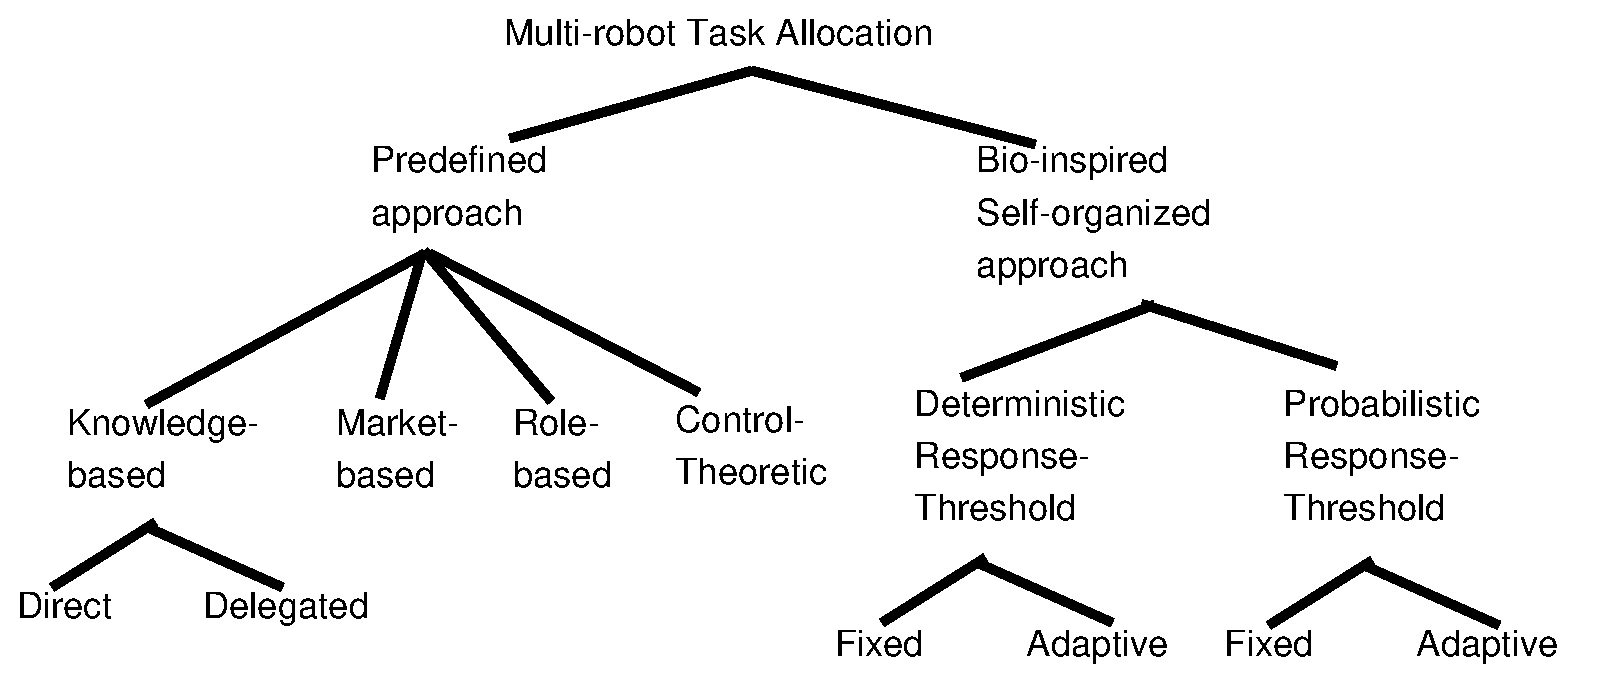
\includegraphics[width=0.7\linewidth, angle=0]
{./images/ta-categories.eps}
\caption{Classification of MRTA solutions.}
\label{fig:mrta-classification} % Give a unique label
\end{figure*}
%%
Since the 90s, many robot control architectures have been designed with thed sole purpose of addressing the MRTA issue from different perspectives. Based on the high-level design of those solutions, we have classified them into two categories: 1) {\em predefined} or {\em explicit} task-allocation and 2) {\em bio-inspired self-organized} task-allocation. Fig. \ref{fig:mrta-classification} illustrates our classification.

In most of the traditional multi-robot systems, task allocation is achieved using well-defined models of tasks and environments. Here it is assumed that the system designer has precise knowledge of tasks and robot-capabilities. Many flavours of this type of task-allocation can be found in the literature. Knowledge-based and multi-agent based approaches use various knowledge-based techniques to represent tasks and robot-capabilities. An early well-known MRTA architecture of this category is ALLIANCE in which each robot models the ability of team-members to perform tasks by observing their current task performances and collecting relevant task quality statistics, e.g., the time it takes a robot to complete a task \cite{Parker1998}. Multi-agent systems also use both centralized and decentralized approaches for allocating tasks among  its  peers. A detailed categorization has been reported in by Shen \citet{Shen+2001} where in a multi-agent task allocation systems are divided into those that use a central supervising agent , those that use a few mediator agents and those that use all independent agents. 

As a feasible alternative to the above multi-agent based task-allocation mechanisms, many researchers have been following the market-based approaches \citet{Dias+2006}.  These approaches originated from the Contract-Net Protocol.  Market-based approaches can be implemented as a centralized auctioning system  as a set of a few auctioneers or as all independent auctioneers.
%For example, in a completely distributed system, when a robot needs to perform a task for which it does not have necessary expertise or resources, it broadcasts a task-announcement message, often with  a expiry time of that message. Robots, that received the message and can perform that task, return a bid message. The initiating robot or {\em  manager} selects one (or more) bidder, called as {\em contractor}, and offers the opportunity to complete the task. The choice of contractor is done by the manager with a mutual agreement with contractor that maximizes the individual profits.

Under role or value-based task-allocation schemes, each role assumes several specific tasks and each robot selects roles that best suit their individual skills and capabilities \cite{Chaimowicz2002}. In this case, robots are typically heterogeneous, each one having variety of different sensing, computation and effector capabilities. In multi-robot soccer \cite{Stone+1999}, positions played by different robots are often defined as roles, e.g. goal-keeper, left/right defender and left/right forward. 

Under control-theoretic approaches, a model of the system is usually developed, that converts the task specification into an objective function to be optimized. This model typically uses the rigid body dynamics of the robots and requires that the mass and other parameters are well-known. Control laws for individual robots are derived either analytically either in advance or at run-time.
%Unlike most other approaches where task-allocation problem is taken as discrete, control-theoretic approaches can produce continuous  solutions. The formalisms of these systems allow system designer to check the system's controllability, stability and related other properties.  These systems typically use some degree of centralization, e.g. choosing a leader robot.  
Control-theoretic approaches have been developed for multi-robot formation control \cite{Belta+2004} and multi-robot box-pushing \cite{Pereira+2003}.
Predefined task-allocation through other approaches are also present in the literature. For example, inspired by the vacancy chain phenomena in nature, a vacancy chain scheduling algorithm has been applied to a restricted class of MRTA problems in spatially classifiable domains \cite{Dahl+2004}.

Task performance in self-organized approaches relies on the collective behaviours resulting from the local interactions of many simple and mostly homogeneous or interchangeable agents. Robots choose their tasks independently using general principles of self-organization such as: positive and negative feedback, multiple interactions among entities and their environment, and randomness or amplification of fluctuations (see label A-D in Fig. \ref{fig:afm-rules}) \cite{Camazine+2001}. Moreover. interaction among individuals and their environment can be modulated by stigmergic, local and global communications.  Among many variants of self-organized task-allocation mechanisms, the most common type is threshold-based task-allocation \cite{Bonabeau+1999}. In this approach, a robot's decision to select a particular task depends largely on its perception of a stimulus, e.g., the demand for a task to be performed, and its corresponding response threshold for that task.

Under the deterministic response-threshold approach, each robot has an activation threshold for each task that needs to be performed. It continuously perceives or monitors the stimulus of all tasks that reflect the relative urgencies of tasks. When a particular task-stimulus exceeds a predefined threshold the robot starts working on that task, typically reducing thie related stimuli. When the task-stimuli falls below the fixed threshold the robot abandons that task. This type of approach has been effectively applied in foraging \cite{Liu+2007,Krieger+2000} and aggregation \cite{Agassounon+2002}. The fixed response threshold can initially be same for all robots \cite{Jones+2000} or they can be different according robot capabilities or the configuration of the system \cite{Krieger+2000}. Adaptive response-threshold models change the thresholds over time.  A robot's response threshold for a given task is often decreased as a result of the robot performing that task.  This enables a robot to select that particular task more frequently or in other words specialise on that task \cite{Bonabeau+1999,Agassounon+2002}.

Unlike the deterministic approach, where robots respond preditably, e.g., to the task stimulus that is the furthest above its threshold, probabilistic or stochastic approaches offer a selection process based-on a probability distribution over the tasks.  In this case, all tasks commonly have at least a small, non-zero probability of being chosen.  This random element typically prevcents starvation of low=stimulus tasks.

Explicit task-allocation mechanisms require a known or controlled environment where it is possible to model the tasks, the robots and the environment.  Note that here, tasks can be arbitrarily complex and often require a high level of sensory and processing abilities in the robots.  Robot teamss can consists of homogeneous or heterogeneous individuals, having different capabilities based on the variations in their hardware or software, but the uncertainty of the environment is reduced to a minimum. 

Bio-inspired, self-organized MRTA mechanisms, on the other hand, rely to a much smaller degree on modelling the environment, tasks or robot capabilities.  Most existing research in this area considers a single global task e.g. foraging, area cleaning and box-pushin with the focus of the work being the design of individual robot controllers that can accomplish the task \cite{Gerkey+2003}. More research is needed to study the perfomance of the self-organized approach in handling several different tasks. %At this moment, the bottom line remains as ``select simple robots for simple tasks (self-organized approach) and complex robots for complex tasks (predefined approach)''.
%%
\begin{figure*}
\centering
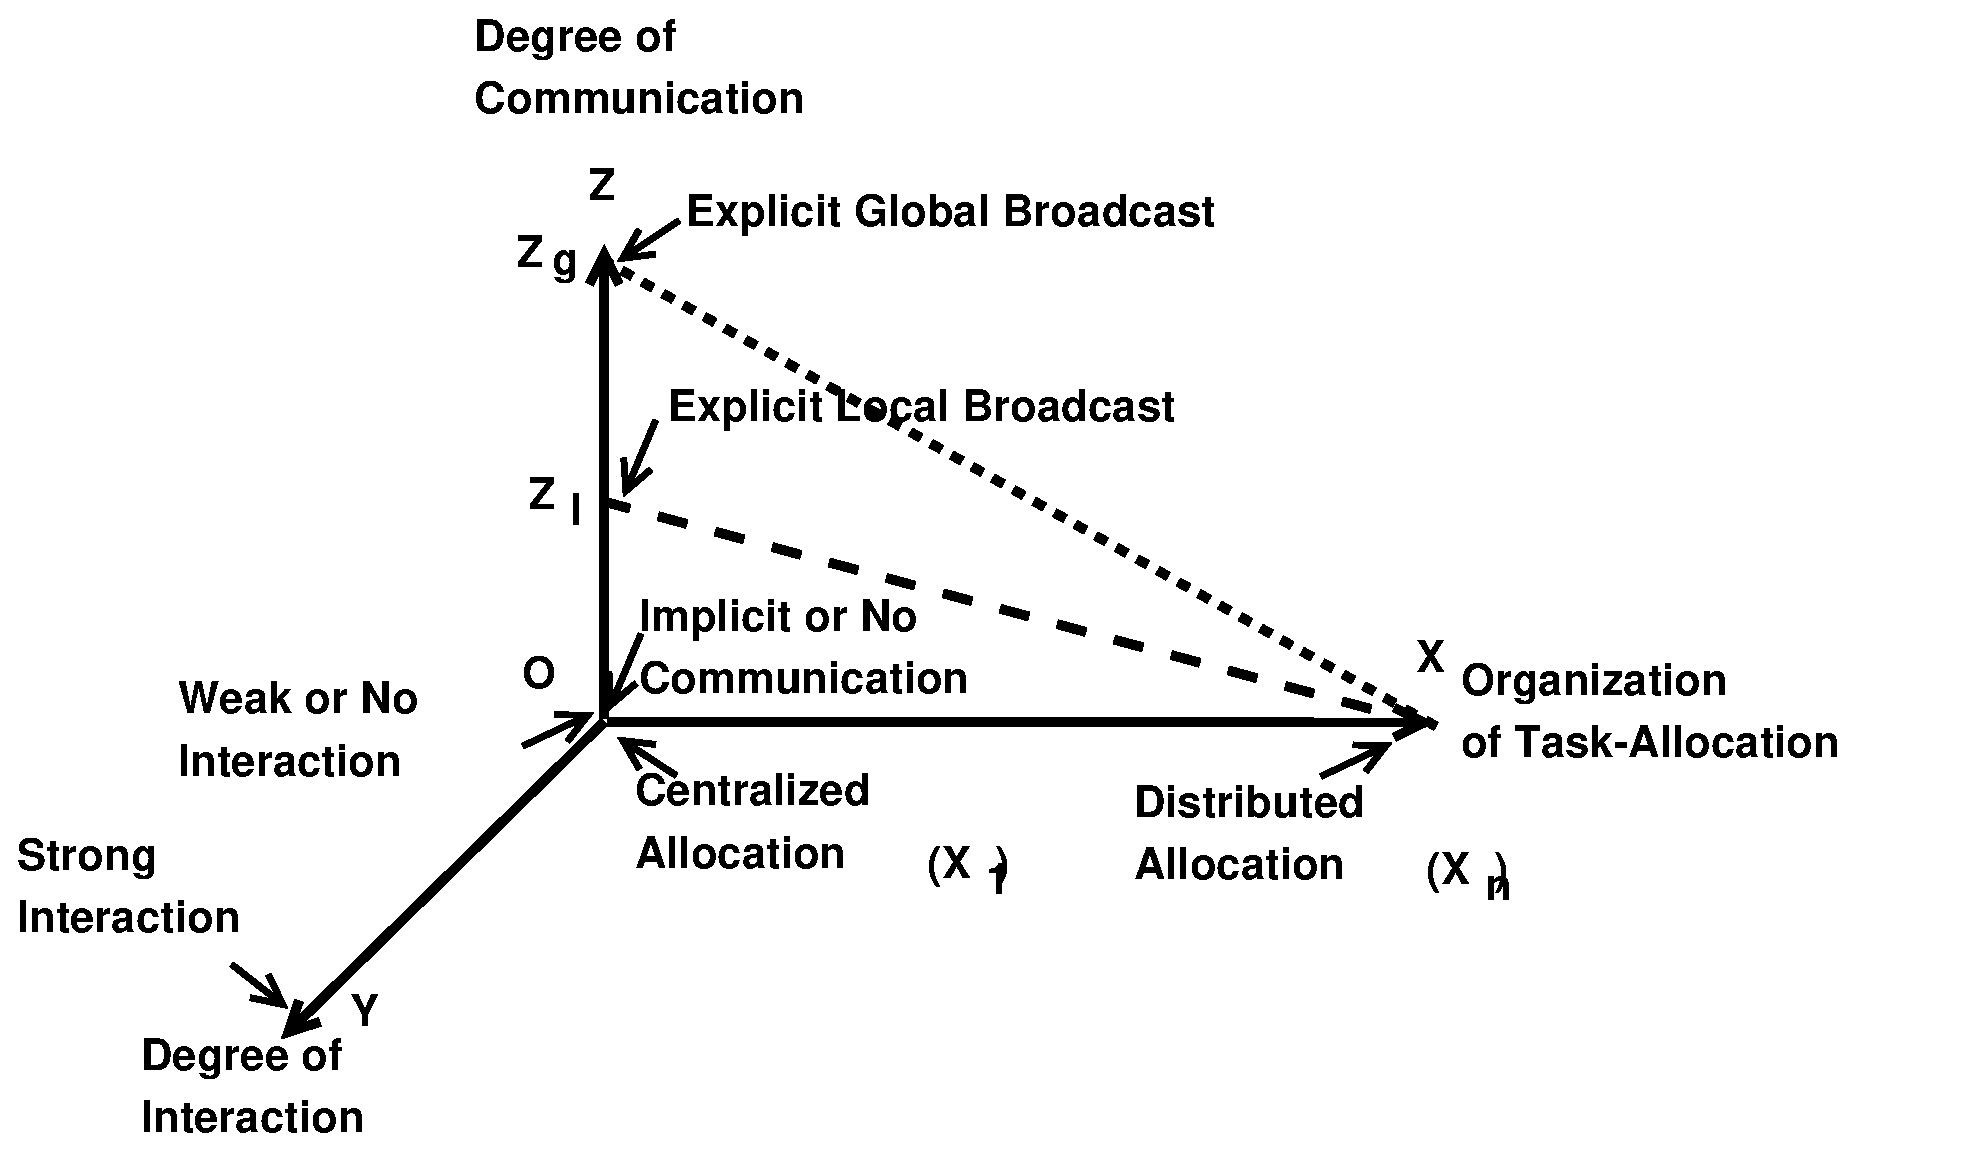
\includegraphics[width=0.7\linewidth, angle=0]
{./images/mrta-lines.eps}
%figure caption is below the figure
\caption{ Three major axes of complexities in MRTA}
\label{fig:mrta-complexities} % Give a unique label
\end{figure*}

Both of the above task-allocation approaches expose their relative strengths and weaknesses when they are put under real-time experiments with variable number of robots and tasks. In an arbitrary event handling domain, a comparison between self-organized and predefined market-based task-allocation was reported by Kalra and Martinoli \citet{kalra+2007}.  They found that explicit task-allocation was more efficient when the required information could be captured accurately.  The threshold-based approach offered similar quality of allocation at a fraction of cost in noisy environment.  

Gerkey and Mataric have presented a study \cite{Gerkey+2003} that compared the complexity and performance of key architectures, including ALLIANCE \cite{Parker1998}, the Broadcast of local eligibillity (BLE) arcgutecture \cite{Werger2001}, M+ \cite{Botelho+1999}, MURDOCH \cite{Gerkey+2002}, First piece auctions \cite{Zlot+2002} and Dynamic role assignment \cite{Chaimowicz2002}.  All of these rely on explicit task-allocation mechanisms. The computational and communication requirements of these MRTA systems were expressed as a function of the number of robots and tasks.  Although the study did not explicitly measure the scalability of the architectures, it clearly showed that many explicit task-allocation mechanisms fail to scale well in environments where the number of robots and tasks are large, given limited overall communication bandwidth and limited processing power for individual robots.

%From above discussions we can see that, self-organized task-allocation methods are advantageous as they can provide fully distributed, scalable and robust MRTA solutions through redundancy and parallelism in task-executions. Moreover, the interaction and communication requirements of robots can also be kept under a minimum limit.  So for large multi-robot system, self-organized task-allocation methods  can potentially be selected, if the complex tasks can be divided into simple pieces that can be carried out by multiple simple robots in parallel with limited communication and interaction requirements.
%%================================================
\section{A Taxonomy of MRTA Approaches}
\label{sec:taxonomy}
In order to understand the interplay among task-allocation, communication and interaction of a particular MRTA approach we have presented these aspects in two 2D characteristic plots.  From this classification we can get an insight about the complexities involved in various kinds of MRTA problems and  the design choices involved in them.
%%
\begin{figure*}[t]
\begin{minipage}[t]{0.48\linewidth}
\centering
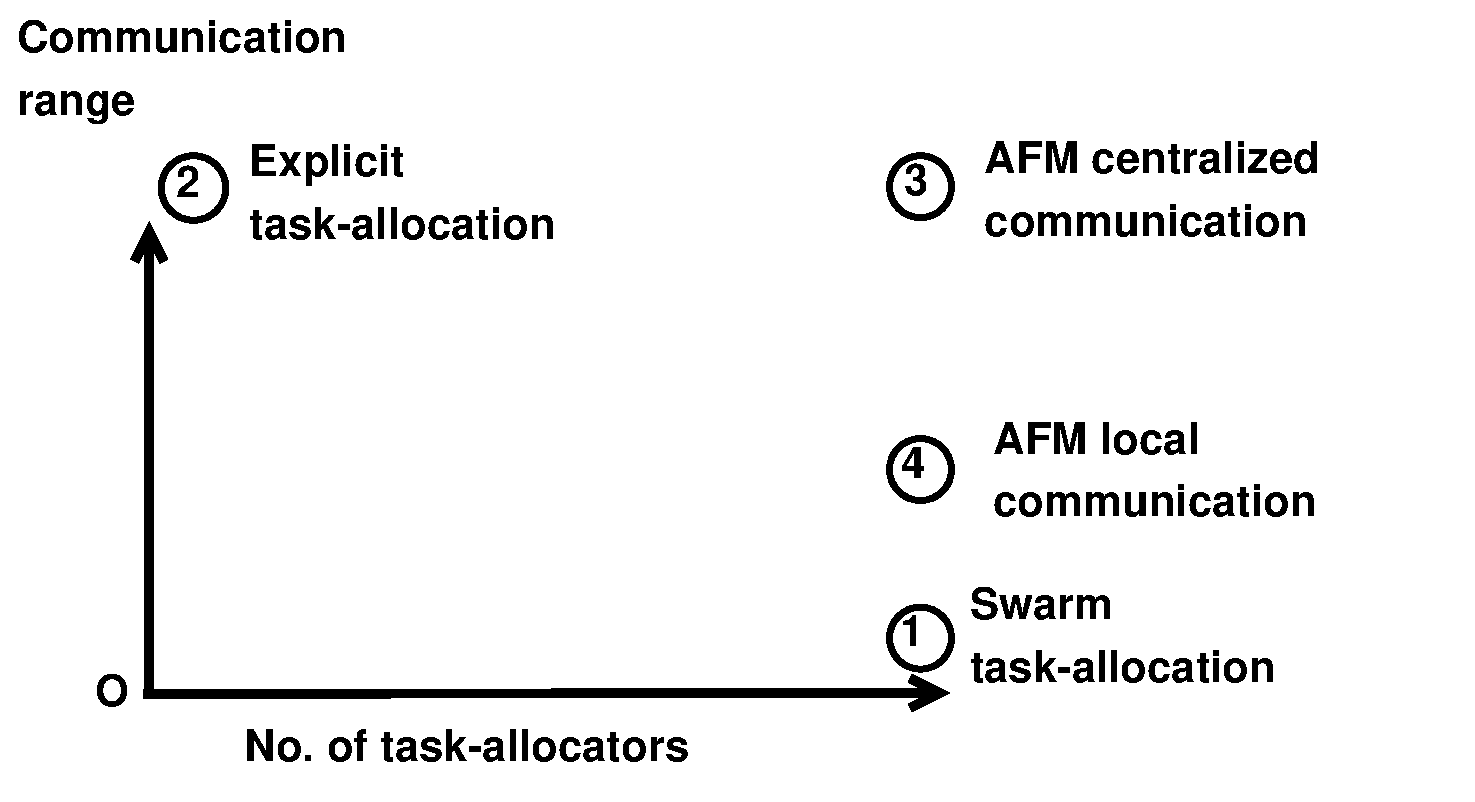
\includegraphics[width=0.99\linewidth, angle=0]
{./images/taxonomy-ta-comm-OK.eps}
%figure caption is below the figure
\caption{Classification of MRTA solutions based on task-allocation and communication strategies}
\label{fig:taxonomy-ta-comm} % Give a unique label
\end{minipage}
%\end{figure}
%\begin{figure}[t]
\begin{minipage}[t]{0.48\linewidth}
\centering
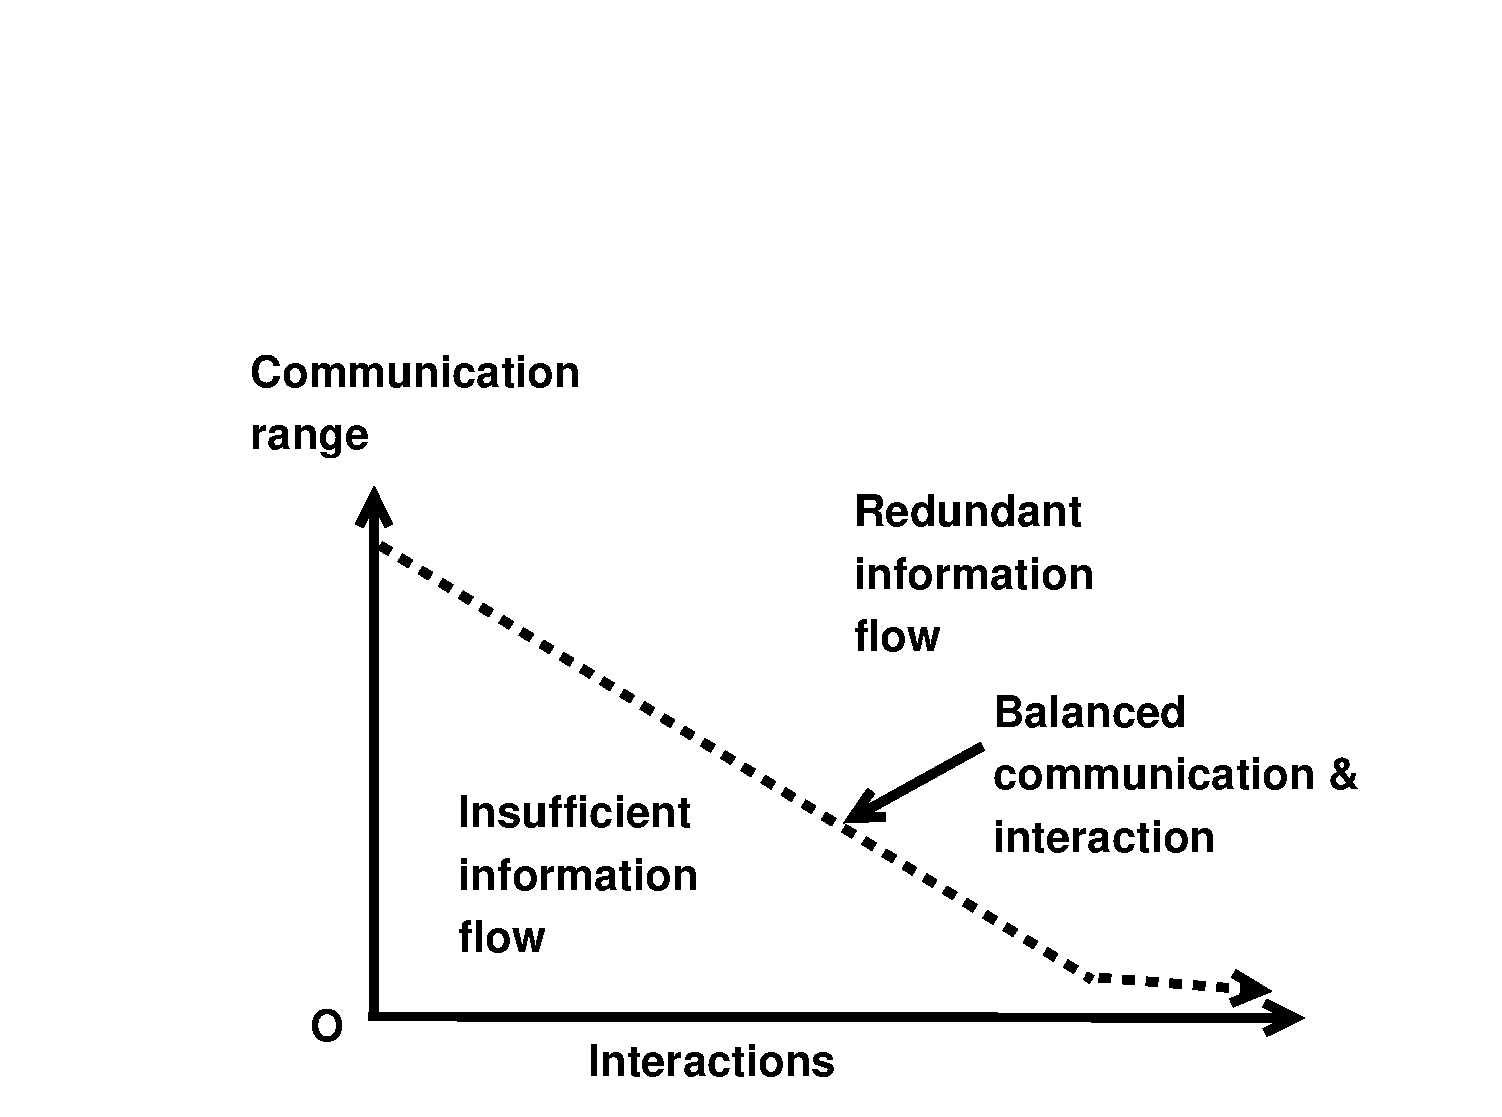
\includegraphics[width=0.99\linewidth, angle=0]
{./images/taxonomy-comm-interaction-OK.eps}
%figure caption is below the figure
\caption{Information flow caused by different levels of communication and interaction}
\label{fig:taxonomy-comm-interaction} % Give a unique label
\end{minipage}
\end{figure*}
%%
Fig. \ref{fig:taxonomy-ta-comm} presents the classification of MRTA solutions based on task-allocation and communication strategies used to disseminate information. Here horizontal axis shows the number of active nodes that provides the task-allocation to the group . The origin of this axis represents the explicit task-allocation by a single centralized entity. For example, in any explicit task-allocation approach, we can use one external centralized entity or one of the robots (aka {\em leader}) to manage the task-allocation. In many predefined methods, e.g. in market-based systems, multiple nodes can act as mediators or task-allocators. Under predefined task-allocation approach, a small number of robots can have fully distributed task-allocation where each robot acts as an independent task-allocator (e.g. as in ALLIANCE architecture). 
The right extreme of horizontal axis in Fig. \ref{fig:taxonomy-ta-comm} represents the swarm task-allocation method which is fully distributed, i.e. each robot selects its tasks independently and without the help of a leader. However, robots might be dependent on other entities for getting the latest {\em information} about tasks. In a recent study on swarm-robotic flocking,  \citet{Celikkanat+2008} show that a swarm can be guided to a target by a few informed individuals or leaders while the remaining robots remain self-organized. Task-allocation in a swarm of robots through one central entity may be rare since one of the major motivations behind swarm robotic systems is to make the swarm task-allocation more robust by avoiding single point of failure.
The vertical axis in Fig. \ref{fig:taxonomy-ta-comm} shows the communication range of individual entities. In case of implicit communication via stigmergy in swarm task-allocation this range does not exist. On the other hand, in case of explicit task-allocation a global range can cover all entities. In this research we have placed our two kinds of experiments vertically aligned with swarm task-allocation. AFM centralized communication represents a GSNC system where communication range is global and task-allocation is fully distributed. Similarly, AFM local communication also represents the the fully distributed task-allocation but with limited communication range under LSLC strategy.

The information flow caused by different levels of communication and interaction has been depicted in Fig. \ref{fig:taxonomy-comm-interaction}. This group-level interaction can be  classified  into  four types: {\em collective}, {\em cooperative}, {\em coordinative} and {\em collaborative} \cite{Parker2008}. From this plot we can see two extremes of information flow. Insufficient information flow occurs when individual's communication range is low and their interaction is limited. In such cases, system designed can find suitable trade-off to get a balanced information flow by increasing  communication range or interaction frequency or both.   On another extreme of this situation we can find lot of redundant information flow where all individuals are both communicating and interacting. Thus the dotted line in the plot refers to a balanced communication and  interaction. This dotted line does not completely intersect the horizontal line since when the communication range is limited to the next neighbour, individuals can still continue to interact with others as much as possible. 

The presence of interaction can be due to the nature of the problem, e.g. cooperation is necessary in co-operative transport tasks. Alternately, this interaction can be a design choice where interaction can improves the performance of the team, e.g. cooperation in cleaning a work-site is not necessary but it can help to improve the efficiency of this task. This plot can also be used to refer to the degree of coupling present in the system. In case of collective interaction, robots merely co-exist, i.e. they may not be aware of each other except treating others as obstacles. Many multi-robot systems are loosely-coupled where robots can indirectly infer some states of the environment from their team-mates' actions. But in many cases, e.g. in co-operative transport, robots not only recognize others as their team-mates, but also they coordinate their actions. Thus they form a tightly coupled system. This level of interaction and coupling also gives us the information about potential side-effects of failure of an individual robot. Tightly coupled systems with high degrees of interactions among the robots suffer from the performance loss if some of the robots removed from the system.

The communication overhead can be resulted from the interactions of robots under a given task-allocation method. Various task-allocation methods rely upon variable degrees of robot-robot communications. On the other hand, the communication capabilities of individual robots can limit (or expand) the level of interaction can be made in a given group. Thus in one way, considering the interaction requirements of a MRTA problem, the system designer can select suitable communication strategies that both minimizes the communication overhead and maximizes the performance of the group. And in other way, the communication capabilities of robots can guide a system designer to design interaction rules of robot teams, e.g. the specification of robot's on-board camera can determine the degree of possible visual interactions among robots. The suitable trade-off between these two axes: communication range and interaction can give us a balanced design of our MRTA solution.
%%============================================================
\section{Robotic interpretation of the Attractive Field Model}
\label{sec:afm}
%%
The AFM has been developed through a collaborative between the partners on the 'Defying the Rules: How Self-Regulated Social; Systems Work' project.  Experiments on ants colonies {\em Temnothorax albipennis} studied the collective performance of ants during brood-sorting and nest construction after emigration to a new site.  The model is also inspired by observational data from the self-organized development of the infrastructure of an {\em eco-village} by an open community of volunteers.  These studies helped us to formalize the a set of necessary and sufficient requirements for self-organisation in a social systems.  We also developed a concrete model of self-organisation based on task-allocation.  This model was validated by deploying it as a robot controller mechanism.  In this section, we describe the generic AFM and how it embodies the requirements for self-organization.  We also provide an interpretation of AFM in multi-robot systems.
\subsection{The Attractive Field Model}
\label{afm:framework}
Inspired from the DOL in ants, humans and robots, we have proposed the following necessary and sufficient set of four requirements for self-regulation in social systems.

\textbf{Requirement 1: Concurrence} The simultaneous presence of several options is necessary in order to meaningfully say that the system has organised into a recognisable structure.   In task-allocation terms the minimum requirement is a single task as well as the option of not performing any task.

\textbf{Requirement 2: Continuous flow of information} Self-organised social systems establish a flow of information over the period of time when self-organisation can be defined.  The task information provides the basis on which the agents self-organise by enabling them to perceive tasks and receive feedback on system performance.

\textbf{Requirement 3: Sensitization} The system must have a way of representing the structure produced by self-organisation, in terms of MRTA, which tasks the robots are allocated.  One of the simplest ways of representing this information is an individual preference parameter for each task-robot combination.  A system where each robot has different levels of preference or {\em sensitivity} to the available tasks, can be said to have to embody a distinct organisation through differentiation.

\textbf{Requirement 4: Forgetting} When a system self-organises by repeated increases in individual sensitisation levels, it is also necessary, in order to avoid saturation, to have a mechanism by which the sensitisation levels are reduced or {\em forgotten}.  In addition to avoiding the situation where a structure produced by self-organisation is eroded by an eventual increase of sensitisation values to a given maximum, forgetting also allows flexibility in the system, in that the structure can change as certain tasks become important and other tasks become less so.  This effect can be achieved by mechanisms such as a slow general decay of sensitisation values or explicit negative feedback.

%%
\begin{figure}
\centering
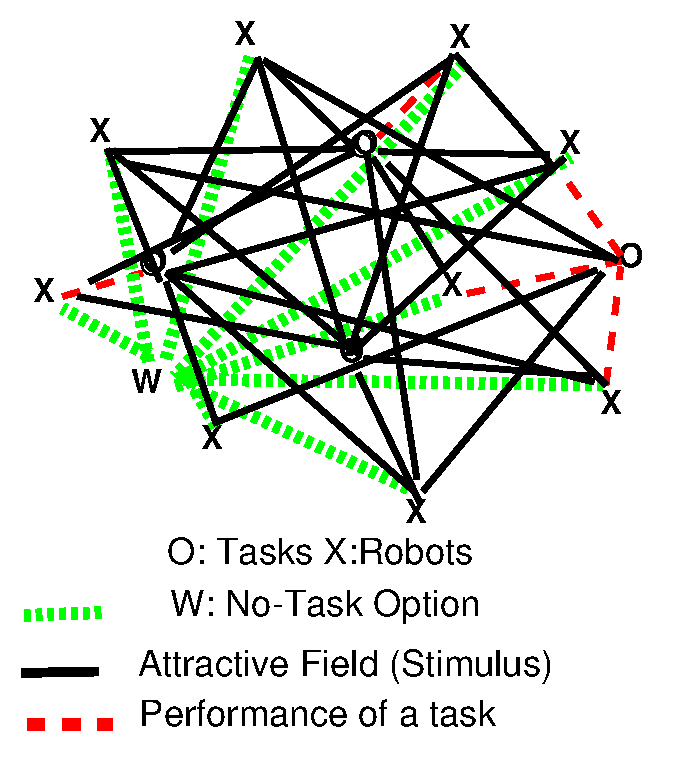
\includegraphics[width=0.7\linewidth, angle=0]{./images/AFM-Diag2.eps}
\caption{The attractive filed model (AFM)}
\label{fig:afm} % Give a unique label
\end{figure}

Building on the requirements for self-organised social systems, AFM formalises these requirements in terms of the relationships between properties of individual agents and of the system as a whole \citet{Arcaute+2008}.  AFM is a bipartite network, i.e. there are two different types of nodes.  One set of nodes describes the sources of the attractive fields, the tasks, and the other set describes the agents.  Edges only exist between different types of nodes and they encode the strength of the atrractive field as perceived by the agent.  There are no edges between agent nodes.  All communication is considered part of the attractive fields.  There is also a permanent field representing the {\em no-task} option of not working in any of the available tasks.  This option is modelled as a random walk.  The model is presented graphically in Fig. \ref{fig:afm}.  The elements depicted are:
\begin{enumerate}
\item Source nodes (o) are tasks to be allocated to agents
\item Agent nodes (x) e.g., ants, humans, or robots
\item Black solid edges represent the attractive fields and correspond to an agent's perceived stimuli from each task.
\item Green edges represent the attractive field of the ever present no-task option, reresented as a particular task (w).
\item The red lines are not edges, but represent how each agent is allocated to a single task at any point in time.
\end{enumerate}

The edges of the AFM network are weighted and the value of this weight describes the strength of the stimulus as perceived by the agent.  In a spatial representation of the model, the strength of the field depends on the physical distance of the agent to the source.  In information-based models, the distance can represent an agent's level of understanding of that task.  The strength of a field is increased through the sensitisation of the agent through experience with performing the task.  This elements is not depicted explicitly in Figure~\ref{fig:afm} but is represented in the weights of the edges.  In Figure~\ref{fig:afm}), the nodes have arbitrary positions.  Even though the distance is physical in this case, it need not be.  When the model is applied to other domains, the distance can represent the accessibility of information or the time the information takes to reach the agent. 
In summary, from the above diagram of the network, we can see that each of the agents is connected to each of the tasks. This means that even if an agent is currently involved in a task, the probability that it stops doing it in order to pursue a different task, or to random walk, is always non-zero.

AFM assumed a repeated task selection by indicidual agents.  The probability of an agent chosing to perform a task is proportional to the sttrangth of the task's attractive field, as given by Equation~\ref{eqn:afm3}.
\begin{equation}
P_{j}^{i} = \frac{S_{j}^{i}}{\sum_{j=0}^{J} S_{j}^{i}} \hspace*{0.25cm}where,\hspace*{0.25cm}S^{i}_{0} = S^{i}_{RW}   
\label{eqn:afm3}
\end{equation}
Equation~\ref{eqn:afm3} states that the probability of an agent, $i$, selecting a task, $j$, is proportional to the stimulus, $ S^i_j$, perceived from that task, with the sum of all the task stimuli normalised to $1$.

The strength of an attractive field varies according to how sensitive the agent is to that task, $k_{j}^{i}$, the distance between the task and the agent, $d_{ij}$, and the {\em urgency}, $\phi _{j}$ of the task.  In order to give a clear edge to each field, its value is modulated by the hyperbolic tangent function, $tanh$.  Equation~\ref{eqn:afm1} formalises this part of AFM.
%% S
\begin{equation}
S_{j}^{i} = tanh\{\frac{k_{j}^{i}}{d_{ij}+\delta } \phi _{j}\}
\label{eqn:afm1}
\end{equation}
Eqation~\ref{eqn:afm1}, used small constant $\delta$, called {\em delta distance}, to avoid division by zero, in the case when a robot has reached to a task.

Equation~\ref{eqn:afm2} shows how AFM handles the the no-task, or random walk, option.  The strength of the stimuli of the random walk task depends on the strengths of the fields real tasks.  In particular, when the other tasks have a low overall level of sensitisation, i.e., relatively weak fields, the strength of the random walk field if relatively high.  On the other hand, when the agent is highly sensitised, the strength of the random walk field becomes relatively low.  We use $J$ to denote the number of real tasks.  AFM effectively considers random walking as an ever present additional task.  Thus the total number of tasks becomes $J+1$. %--P(Task)
\begin{equation}
S^{i}_{RW} = tanh \left \{ 1 -  \frac{ \sum_{j=1}^{J} S^{i}_{j}}{J + 1} \right \}
\label{eqn:afm2}
\end{equation}
%-- P(RW)

A task $j$ has an associated urgency $\phi_j$ indicating its relative importance over time.  If an agent attends a task $j$ in time step $t$, the value of $\phi_j$ will decrease by an amount $\delta_{\phi_{INC}}$ in the time-step $t+1$.  On the other hand, if a task has not been served by any of the agents in time-step $t$, $\phi_j$ will increase by a different amount, $\delta_{\phi_{DEC}}$ in time-step $t+1$.  This behaviour is formalised in Equations~\ref{eqn:delta-phi1} and~\ref{eqn:delta-phi2}.
\begin{equation}
 If\hspace*{0.15cm}the\hspace*{0.15cm} task\hspace*{0.15cm}is\hspace*{0.15cm}not\hspace*{0.15cm}being\hspace*{0.15cm} done:\hspace*{0.15cm} \phi_{j,t+1} \rightarrow \phi_{j,t} \hspace*{0.15cm} + \delta_{\phi_{INC}}
\label{eqn:delta-phi1}
\end{equation}
%%
\begin{equation}
 If\hspace*{0.15cm}the \hspace*{0.15cm}task\hspace*{0.15cm}is\hspace*{0.15cm}being\hspace*{0.15cm}done:\hspace*{0.15cm}  \phi_{j,t+1} \rightarrow \phi_{j,t} \hspace*{0.15cm} - n\hspace*{0.10cm}\delta_{\phi_{DEC}}
\label{eqn:delta-phi2}
\end{equation}
Equation~\ref{eqn:delta-phi1} refers to a case where no agent attends to task $j$ and Equation~\ref{eqn:delta-phi2} to the case where $n$ agens are concurrently performing task $j$.

In order to complete a task, an agent needs to be within a fixed distance of that task.  When an agent performs a task, it learns about it and this will increases the probability of that agent selecting that task in the future.  This is done by increasing its sensitization to the task by a fixed amount, $k_{INC}$. The variable affinity of an agent, $i$, to a task, $j$, is called its {\em sensitization} to that task and is denoted $k^{i}_{j}$.  If an agent, $i$, does not do a task $j$, $k^i_j$ is decreased by a different fixed amount, $k_{DEC}$.  This behaviour is formalised in Equations~\ref{eqn:k-inc} and~\ref{eqn:k-dec}.
\begin{equation}
 If\hspace*{0.15cm}task\hspace*{0.15cm}is\hspace*{0.15cm}done:\hspace*{0.15cm}  k^i_j \rightarrow   k^i_j \hspace*{0.15cm} + \hspace*{0.15cm} k_{INC}
\label{eqn:k-inc}
\end{equation}
\begin{equation}
 If\hspace*{0.15cm}task\hspace*{0.15cm}is\hspace*{0.15cm}not\hspace*{0.15cm}done:\hspace*{0.15cm}  k^i_j \rightarrow   k^i_j \hspace*{0.15cm} - \hspace*{0.15cm} k_{DEC}
\label{eqn:k-dec}
\end{equation}

\subsection{A Robotic Interpretation of AFM}
\label{afm:mrs-interpretation}
The interpretation of AFM in a multi-robot system follows the above mentioned generic interpretation.  Each robot is modelled as an agent and each task is modellled as a spatial location.  The robots repeatedly select tasks and if the robot is outside a fixed task boundry, it navigates towards the task.  If the robot is within the task boundry it remains there until the end of the time step when a new (or the same) task is selected.
The distance between a task and a robot is simply the physical distance and the sensitivities are recorded as specific values on each robot.
The urgency values of the tasks are calculated based on the number of robots attending each task and the updated urgency values are communicated to the robots.

The sensing of the distance between the taks and robots as well as the communication of urgency values are non-trivial in a robotic systen.  Both the sensing and communication can be done either locally by the individual robots or centrally, through an overhead camera and a global communication network.
This article presents work on exploring the effects of different sensing and communication models on the performance of MRTA systems.

%%--------------------------------------------------------------------
\subsection{AFM and Biological Self-Organization}
\label{afm:so}

Fig.  \ref{fig:afm-rules} labels the four distinct perspectives known as so-called ingredients or properties of self-organization:  A) positive feedback, B) negative feedback, C) presence of multiple interactions among individuals and their environment, and D) amplification of fluctuations  e.g., random walks, errors, random task-switching \cite{Camazine+2001}. However, it is not clear how those properties can come into existence. Fig.  \ref{fig:afm-rules} depicts  the four underlying mechanisms (label 1 to 4) that explain how self-organization can be realized in different social systems using our generic framework. These are explained in the following paragraphs.

Firstly, multiple interactions become meaningful when {\em continuous flow of information} occurs  by exchanging signals or cues among agents or their environment  that regulates their behaviours. This, in turn, contribute to the task-allocation  and task-switching in the social level.  In swarm intelligence literature, multiple interactions are often described as an essential ingredient of self-organization. However, interactions without definite purposes may not contribute to the self-organization.

Secondly, in swarm intelligence, positive feedback has been attributed as another mechanism of  self-organization. But it is not easy to understand what creates positive feedback in a social system. Possible answers might be the characteristic of the environment e.g. ants select shorter path since density of pheromones becomes higher and thus more ants becomes attracted in that path, by causing the gradual decrease of response-threshold of individuals. This increases the probability of selecting a task.  To make the answer more specific, we have explicitly attributed {\em sensitisation} or learning as a mechanism of positive feedback. There might exist other mechanisms too. But clearly sensitisation will be one of the reliable mechanisms for achieving positive feedback.

Thirdly, similar to positive feedback, we have proposed {\em forgetting} that contributes to provide negative feedback about a task or decreasing the probability to select it. Other negative feedback mechanisms can be implemented by assigning a saturation level to each task which is also present in our model, for details see \citet{Arcaute+2008}.

Finally, creating  artificial amplification of fluctuations or stochastic events is not a straight-forward issue. It throws  many open questions. Does a system designer intentionally impose irregularity in task-performance of agents?  Is random movement  enough for simulating randomness in a system?
Since emergencies do not always pop-up on request, we provide the rule of {\em concurrency} that enables agents to  maintain even a small amount of probability of selecting a low-priority, or less sensitized or distant task. This concurrency mechanism provides a high-degree of robustness in the system such that all tasks can be attended even if specialization of agents delays them in switching to some of the tasks.
%%

%%============================================================ 
\section{A Manufacturing Shop-Floor Interpretation of AFM}
\label{sec:mrta}
We have designed a set of  manufacturing shop-floor scenario experiments for validating the effectiveness of our AFM in producing self-regulated MRTA.  In this section, we have described our manufacturing shop-floor scenario and our task-allocation solution for robot-controllers.
%%
\begin{figure*}
\centering
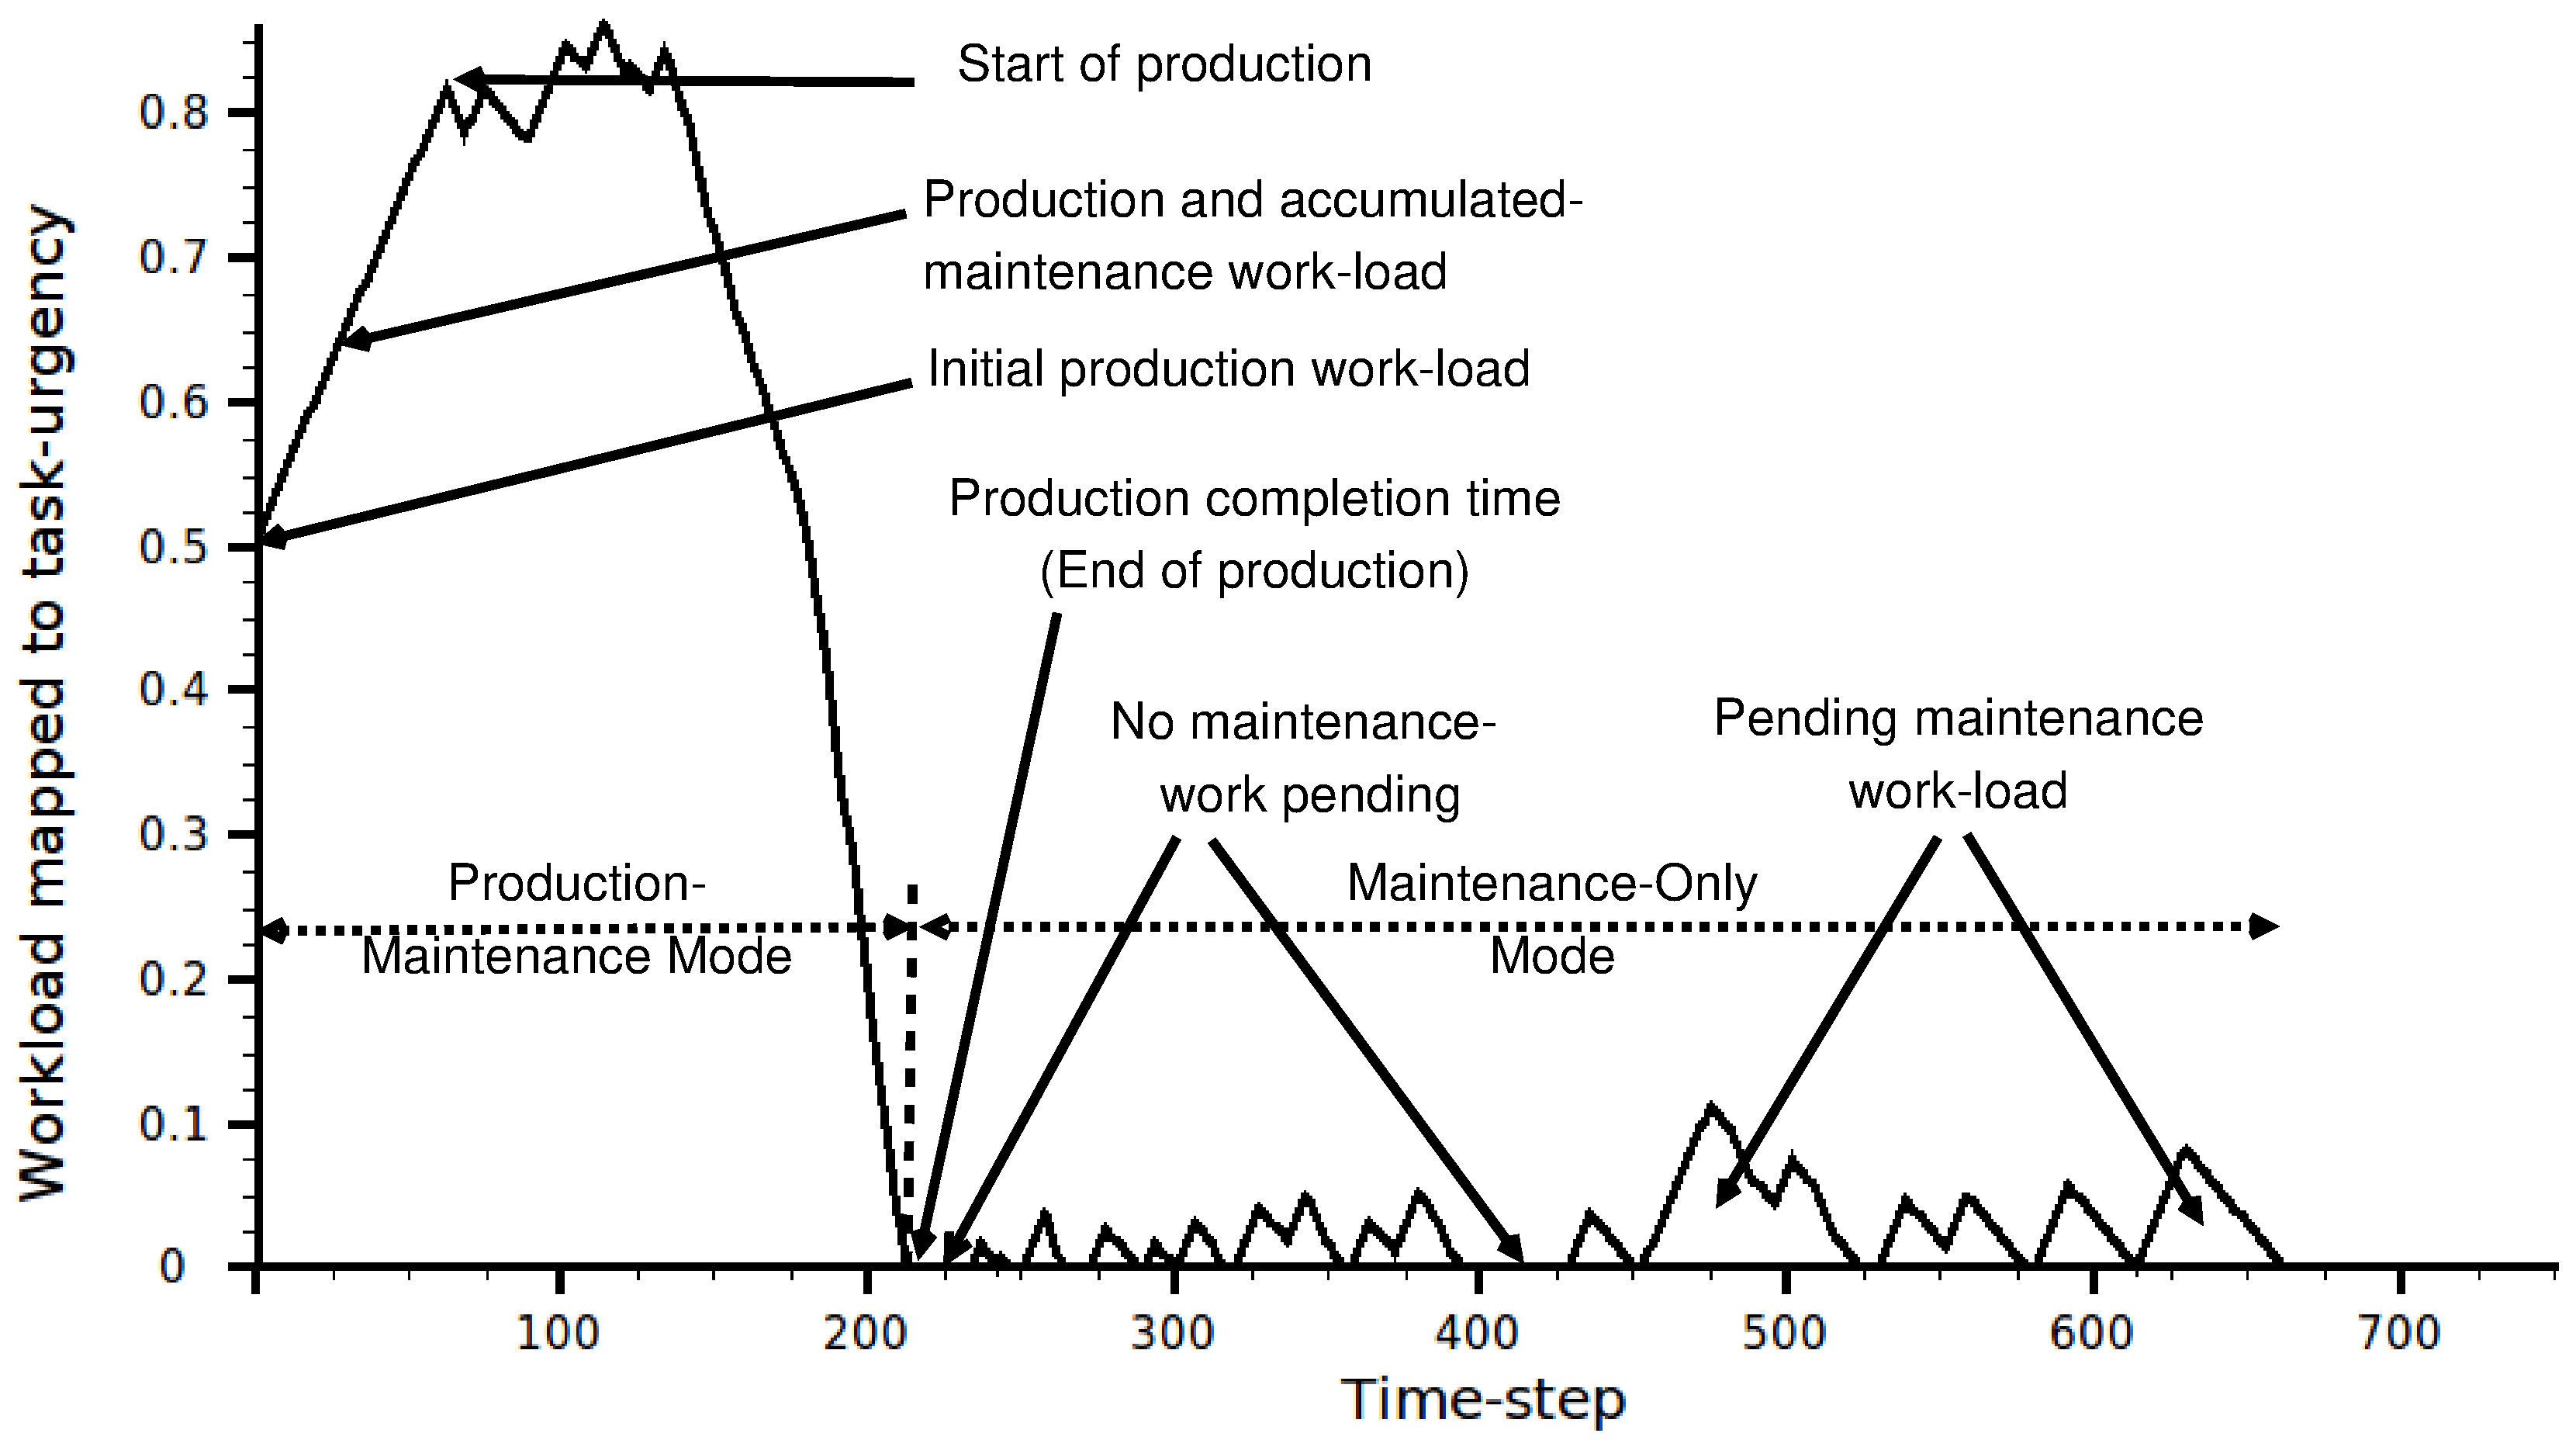
\includegraphics[width=0.7\linewidth, angle=0]
{./images/VSP.eps}
%figure caption is below the figure
\caption{A manufacturing shop-floor production and maintenance cycle}
\label{fig:vsp}  % Give a unique label
\end{figure*}
%--------------------------------------------
\subsection{A manufacturing shop-floor scenario}
\label{afm:vms}
By extending our interpretation of AFM in multi-robot system, we can set-up manufacturing shop-floor  scenario. Here, each task represents a manufacturing machine that is  capable of producing goods from raw materials, but they also require constant maintenance works for stable operations. Let $W_{j}$ be a finite number of material parts that can be loaded into a machine $j$ in the beginning of its production process and in each time-step, $\omega_{j}$ units of material parts can be processed  ($\omega_{j} \ll W_{j} $). So let $\Omega_{j}^{p}$ be the initial production workload of $j$ which is simply: $W_{j} / \omega_{j}$ unit.

We assume that all machines are identical. In each time step, each machine always requires a minimum threshold number of robots, called hereafter as {\em minimum robots per machine ($\mu$)}, to meet its constant maintenance work-load, $\Omega_{j}^{m}$ unit. However, if $\mu$ or more robots are present in a machine for production purpose, we assume that, no extra robot is required to do its maintenance work separately. These robots, along with their production jobs, can do necessary maintenance works concurrently. For the sake of simplicity, here we consider $\mu$ = 1.

Now let us fit the above production and maintenance work-loads and task performance of robots into a unit task-urgency scale. Let us divide our manufacturing operation into two subsequent stages: 1) \acfi{PMM}, and 2) \acfi{MOM}. Initially a machine starts working in PMM and does production and maintenance works concurrently. When there is no production work left, then it  enters into MOM. Fig. \ref{fig:vsp} illustrates this scenario for a single machine.

Under both modes, let $\alpha_{j}$ be the amount of workload occurs in a unit time-step if no robot serves a task and it corresponds to a fixed task-urgency $\Delta \phi_{INC}$. On the other hand, let us assume that in each time-step, a robot, $i$, can decrease a constant workload $\beta_{i}$ by doing some maintenance work along with doing any available production work. This  corresponds to a negative task urgency: $- \Delta \phi_{DEC}$. So, at the beginning of production process, task-urgency, occurred in a machine due to its production work-loads, can be encoded by Eq. \ref{eqn:task-urgency-prod-init}.
\begin{equation}
%\small
\Phi_{j, INIT}^{PMM} = \Omega_{j}^{p} \times \Delta \phi_{INC} + \phi_{j}^{m0}
\label{eqn:task-urgency-prod-init}
\end{equation}
where $\phi_{j}^{m0}$ represents the task-urgency due to any initial maintenance work-load of $j$.
Now if no robot attends to serve a machine, each time-step a constant maintenance workload of $\alpha_{j}^{m}$ will be added to $j$ and that will increase its task-urgency by $\Delta \phi_{INC}$. So, if $k$ time steps passes without any production work being done, task urgency at $k^{th}$ time-step will follow Eq. \ref{eqn:task-urgency-prod-case1}.
\begin{equation}
\Phi_{j, k}^{PMM} =\Phi_{j, INIT}^{PMM} + k \times \Delta \phi_{INC}
\label{eqn:task-urgency-prod-case1}
\end{equation}
However, if a robot attends to a machine and does some production works from it, there would be no extra maintenance work as we have assumed that $\mu$ = 1. Rather, the task-urgency on this machine will decrease by $\Delta \phi_{DEC}$ amount. If $\nu_{k}$ robots work on a machine simultaneously at time-step $k$, this decrease will be: $\nu_{k} \times \Delta \phi_{DEC}$. So in such cases, task-urgency in $(k+1)^{th}$ time-step can be represented by:
\begin{equation}
\Phi_{j, k+1}^{PMM} = \Phi_{j, k}^{PMM} - \nu_{k} \times \Delta \phi_{DEC}
\label{eqn:task-urgency-prod-case2}
\end{equation}
At a particular machine $j$, once $\Phi_{j, k}^{PMM}$ reaches to zero, we can say that there is no more production work left and this time-step $k$ can give us the {\em production completion time} of $j$, $T_{j}^{PMM}$. Average production time-steps of a shop-floor with M machines can be calculated by the following simple equation.
\begin{equation}
T_{avg}^{PMM} = \frac{1}{M} \sum_{j=1}^{M} T_{j}^{PMM} 
\label{eqn:avg-pmm}
\end{equation}
$T_{avg}^{PMM}$ can be compared with the minimum number of time-steps necessary to finish production works, $T_{min}^{PMM}$. This can only happen in an ideal case where all robots work for production without any random walking or failure. We can get $T_{min}^{PMM}$ from the total amount of work load and maximum possible inputs from all robots. If there are M machines and N robots, each machine has $\Phi_{INIT}^{PMM}$ task-urgency, and each time-step robots can decrease N $\times$ $\Delta \phi_{DEC}$ task-urgencies, then the theoretical $T_{min}^{PMM}$ can be found from the following Eq. \ref{eqn:min-pmm}.
%
%\begin{multicols}{2}
%\small
\begin{equation}
T_{min}^{PMM} = \frac{M \times \Phi_{INIT}^{PMM}}{N \times \Delta \phi_{DEC}} 
\label{eqn:min-pmm}
\end{equation}
%\vspace*{0.2cm}
\begin{equation}
\zeta_{avg}^{PMM} = \frac{T_{avg}^{PMM} - T_{min}^{PMM}}{T_{min}^{PMM}} 
\label{eqn:appd}
\end{equation}
%\end{multicols}
Thus we can define $\zeta_{avg}^{PMM}$, \acf{APCD} by following Eq. \ref{eqn:appd}:
%%
When a machine enters into MOM, only $\mu$ robots are required to do its maintenance works in each time step. So, in such cases, if no robot serves a machine, the growth of task-urgency will follow Eq. \ref{eqn:task-urgency-prod-case1}. However, if $\nu_{k}$ robots are serving this machine at a particular time-step $k^{th}$ , task-urgency at $(k+1)^{th}$ time-step can be represented by:
\begin{equation}
\Phi_{j, k+1}^{MOM} = \Phi_{j, k}^{MOM}- (\nu_{k} - \mu) \times \Delta \phi_{DEC}
\label{eqn:task-urgency-maint-case}
\end{equation}
By considering $\mu = 1$, Eq. \ref{eqn:task-urgency-maint-case} will reduces to Eq. \ref{eqn:task-urgency-prod-case2}. Here, $\Phi_{j, k+1}^{MOM}$ will correspond to the {\em pending maintenance work-load} of a particular machine at a given time. This happens due to the random task switching of robots with a no-task option (random-walking). Interestingly PMW will indicate the robustness of this system since higher PMW value will indicate the delay in attending maintenance works by robots. We can find the \acfi{APMW} per time-step per machine, $\chi_{j}^{MOM}$ (Eq. \ref{eqn:sigle-pmw}) and average PMW per machine per time-step, $\chi_{avg}^{MOM}$ (Eq. \ref{eqn:avg-pmw}).
%\begin{multicols}{2}
%\small
\begin{equation}
\chi_{j}^{MOM}= \frac{1}{K} \sum_{k=1}^{K} \Phi_{j, k}^{MOM}
\label{eqn:sigle-pmw}
\end{equation}
%\vspace*{0.2cm}
\begin{equation}
\chi_{avg}^{MOM}= \frac{1}{M} \sum_{j=1}^{M} {\chi_{j}^{MOM}}
\label{eqn:avg-pmw}
\end{equation}
%\end{multicols}
%----------------------------------------------------------------
\subsection{Robot-controller algorithms}
\label{ss:rcc-alg}
In our task-allocation algorithm, for each task, we extract its pose, urgency, sensitisation from input data. \textit{CalculateTaskDistance()} function calculates the Euclidian distance between a task and a the robot by taking the current robot-pose and static task-pose as the input. These values are enough to get a task's stimuli based on Eq. \ref{eqn:afm1}. We get the random-walk task's stimuli from Eq. \ref{eqn:afm2}.\\

\textbf{Algorithm 1: Self-regulated task-allocation by AFM}
\vspace{-3mm}
\newline
\HRule
\begin{algorithmic}[1]
\begin{small}
\label{alg:task-selector}
\State $\textbf{Input: } AllTaskInfo, RobotPose, TaskRecords, DeltaDistance$
\State $\textbf{Output: } SelectedTaskID$
\State \COMMENT {Stage 1: Get  sum  of stimulus of all tasks}
\State $TotalTasks \gets$  Total number of tasks $\in AllTaskInfo$  
\State $ TaskStimuliSum \gets 0 $
\ForAll {$ Task \in AllTaskInfo $} 
\State $ TaskPose \gets  $ Task-position  $ \in Task$
\State $ TaskUrgency \gets $ Task-urgency $ \in Task$
\State $ TaskSensitization \gets $ Task-sensitization $\in Task$
\State $ DistToTask \gets$
\textbf{CalculateTaskDistance(}
\newline
$RobotPose$, $TaskPose$\textbf{)}
\State $ TaskStimuli \gets  $ \textbf{CalculateTaskStimuli(}
\newline
$DistToTask, TaskSensitization, TaskUrgency, DeltaDistance$\textbf{)}
\State $ TaskStimuliSum \gets$  $TaskStimuliSum + TaskStimuli$
\State $ TaskRecords \gets $ \textbf{UpdateTaskRecords(\\}$TaskStimuli,DistToTask, TaskUrgency,$\\ $TaskSensitization\textbf{)}$
\EndFor
%%
\State $RandomWalkStimuli \gets $ \textbf{CalculateRandomWalkStimuli(\\}$TotalTasks,$ %\hspace*{4.5cm}
 $TaskStimuliSum$\textbf{)}
\State $ AllStimuliSum \gets TaskStimuliSum + RandomWalkStimuli $
%%
\State \COMMENT {Stage 2: Find probability of doing each task }
\State $ TaskID \gets 0 $ 
\While {$ TaskID \leq TotalTasks $} 
\State $ TaskStimuli \gets $ Task-stimuli $\in TaskRecords(TaskID)$
\State $ TaskProbability \gets  $ \textbf{GetTaskProbability(\\}$TaskStimuli, AllStimuliSum$\textbf{)}
\State $ TaskProbabilityRange \gets $
\newline
 \textbf{ConvertTaskProbabilityIntoRange(}\\ $TaskProbability$\textbf{)}
\State $ TaskRecords \gets  $ \textbf{UpdateTaskRecords(}$TaskProbability$\textbf{)}
\EndWhile
%%
\State \COMMENT {Stage 3: Draw a random-number to match TaskID}
\State $ RandomNum \gets  $ 
\newline
\textbf{GetRandomNumber(}$0,$ \textbf{Max(}$TaskProbabilityRange$\textbf{))}
\While {$ TaskID \leq TotalTasks $} 
\State $ RangeStart \gets  $ \textbf{Min(}$TaskProbabilityRange (TaskID)$\textbf{)}
\State $ RangeEnd \gets  $ \textbf{Max(}$TaskProbabilityRange (TaskID)$\textbf{)}
\If {$  RandomNum \geq RangeStart$ \newline $\hspace*{.25cm}\&\& \hspace*{.25cm} RandomNum  \leq  RangeEnd $}
\State $ SelectedTaskID \gets TaskID $ 
\EndIf
\EndWhile
\end{small}
\end{algorithmic}
\vspace{-3mm} 
\HRule\\
%%
In the second stage of our task-allocation algorithm, we  find the probability of each task (including random-walk) based on Eq. \ref{eqn:afm3}. Then this probability value of each task, between 0 and 1, is rounded to the closest two-digit fractions and multiplied by 100 and put into a linear scale. Then we use a random-number generator that draws a random-number between 0 and the highest value of task-probability range. Then this random number is compared against the task probability range of each task. Under this probabilistic method, the task with larger probability range has a  higher chance to be selected, but low probability tasks can also be selected time-to-time.\\

\textbf{Algorithm 2: Robot's learning and forgetting of tasks}
\vspace{-3mm}
\newline
\HRule
\begin{algorithmic}[1]
\begin{small}
\label{alg:update-sz}
\State $\textbf{Input: }  TaskRecords, LeranRate, ForgetRate, SelectedTaskID$
\State $\textbf{Output: }$ Updated $TaskSensitisation \in TaskRecords$
\ForAll {$ Task \in TaskRecords $} 
\State $ TaskID \gets  $ ID $\in Task$
\State $ TaskSensitization \gets  $   Sensitisation $ \in Task$
\If {$  TaskID \equiv SelectedTaskID $}
\State $ TaskSensitization \gets $ \textbf{Max(}$1, (TaskSensitization + LeanRate)$\textbf{)}
\Else
\State $ TaskSensitization \gets $ \textbf{Min(}$0, (TaskSensitization - ForgetRate)$\textbf{)}
\EndIf
\EndFor
\end{small}
\end{algorithmic}
\vspace{-3mm} 
\HRule\\
%%

Algorithm 2 lists the pseudo-code for updating (learning and forgetting) the robot's task-sensitization values. Along with previously mentioned \textit{TaskRecords}, and  \textit{SelectedTaskID}, it takes two other inputs: \textit{LeranRate} ($\Delta k_{INC} $) and \textit{ForgetRate} ($\Delta k_{INC} $) as outlined in Eq. \ref{eqn:k-inc} and \ref{eqn:k-dec} respectively.  In addition to that it also keep the value of task-sensitization between the fixed limit of 0 and 1.
%==============================================================
\section{Centralized communication model}
\begin{figure}
\centering
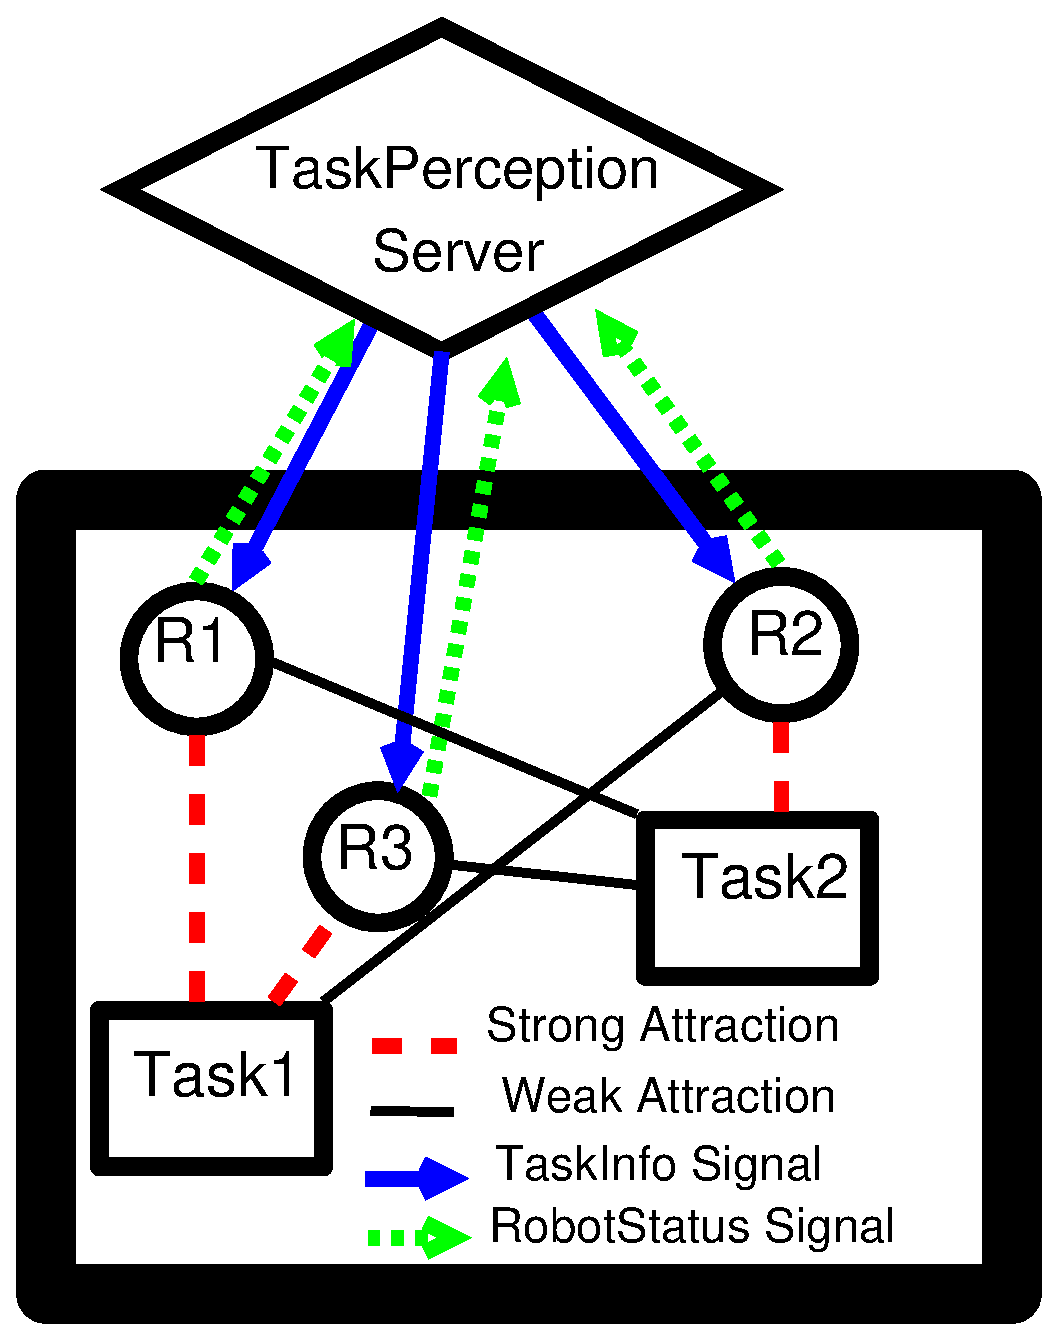
\includegraphics[height=7cm, angle=0]{./images/CentralizedComm.eps}
\caption{\small A centralized communication scheme} % for implementing AFM}
\label{fig:ccm} % Give a unique label
\end{figure}
%%
AFM relies upon a system-wide continuous flow of information which can be realized using any suitable communication model. A simple centralized communication scheme is outlined in Fig. \ref{fig:ccm}. In this model we have used bi-directional signal-based exchange of communication messages between a centralized \textit{task perception server} (TPS) and a \textit{robot-controller client} (RCC). The main role of TPS is to send up-to-date task-information to RCCs. This  task-information mainly contains the location and urgency of all tasks  which is used by the RCCs for running their task-allocation algorithm. The urgency value of each task is dynamically updated  by TPS after receiving the  status signals from the working robots of that particular task. Fig. \ref{fig:ccm} shows how three robots are attracted to two different tasks and their communications with TPS. Here although the robots are selecting task independently based-on the strength of their attractive fields to different tasks, they are depended on the TPS for task-information.
%%
\subsection{General characteristics}
We can characterize our communication model in terms of three fundamental issues of communication \cite{Gerkey+2001}. 
\begin{enumerate}
\item Message content: {\em what to communicate?}
\item Communication frequency: {\em when to communicate?}
\item Target message recipients: {\em with whom to communicate?}
\end{enumerate}
%%
AFM suggests the communication of task-urgencies  among robots. This communication helps the robots to gain information that can be  treated as ``global sensing''. However in this model  robots do not communicate among themselves. Hence this model can be approximated as the GSNC strategy. Since in order to run the task-allocation algorithm robot-controllers need the distance information we also include the task position information in  the message. Our centralized communication model is open to include any further information, such as time-stamp, in the message payload. In this centralized communication model the frequency of signal emission depends on several issues, e.g. the rate at which the environment is changing, the bandwidth of communication medium. In case of time-extended tasks, robots can receive information less frequently and the  bandwidth usage can be kept  minimum. However under a fast changing environment relatively more bandwidth will be required.  Finally the centralized communication model spread the attractive fields of all tasks globally by broadcasting information to all robots.  
%%
\subsection{Algorithm}
The algorithm that updates the task-urgencies in TPS is given here.\\
\textbf{Algorithm 3: Task-urgency update rules based on AFM}
\vspace{-3mm}
\newline
\HRule
%% ALG
\begin{algorithmic}[1]
\begin{small}
\label{alg:tps}
\State $\textbf{Input: } AllTaskInfo, AllTaskWorkers, ThresholdWorkers,$\\ \hspace*{1cm}$DeltaUrgencyINC, DeltaUrgencyDEC$
\State $\textbf{Output: }$ Updated $TaskUrgencies \in AllTaskInfo$
\ForAll {$ (Task, Workers) \in (AllTaskInfo, AllTaskWorkers) $} 
\State $ TaskUrgency \gets $ Task-urgency $\in Task$
\State $ TaskWorkers \gets $ Number of workers $ \in Workers$
\If {$ TaskWorkers < ThresholdWorkers $}
\State $ TaskUrgency \gets $ \textbf{Max(}$1, (TaskUgerncy + DeltaUrgencyINC)$\textbf{)}
\Else
\State $ TaskUrgency \gets $ \textbf{Min(}$0, (TaskUgerncy - $\\ \hspace*{5.3cm}$ TaskWorkers \times DeltaUrgencyDEC)$\textbf{)}
\EndIf
\EndFor
\end{small}
\end{algorithmic}
%%
\vspace{-3mm} 
\HRule\\
%%
The above algorithm relies on the previously mentioned task-status signals from the working robots.  It sorts out the worker robots' robot-id according to their task-id and use the worker count to determine whether the corresponding task-urgency needs any change  according the rules of AFM. For example, here we have shown that if the number of working robots exceeds a pre-set threshold task urgency has been updated based on Eq. \ref{eqn:delta-phi1} and \ref{eqn:delta-phi2}. Moreover, in order to satisfy our interpretation of AFM, the task-urgency values are kept within a fixed range 0 and 1.
%%
\subsection{Implementation strategy}
Our centralized communication model has been implemented by the D-Bus interprocess communication technology \cite{Pennington+2010}. Under this implementation, we have used D-Bus \textit{signal} type asynchronous messages to enable information sharing among SwisTrack multi-robot tracker \cite{Lochmatter+2008}, TPS and RCCs inside a single host. D-Bus signals give us the flexible, fault-tolerant and real-time messaging scheme which can not be easily achieved in other interprocess communication schemes. The detail design of our  D-Bus implementation can be found in \cite{Sarker2010control}. The specific implementation of signals and their payloads are discussed in Sec. \ref{afm:impl}.
%==============================================================
\section{Local P2P communication model (LPCM)}
In most swarm robotic research local communication is considered as the one of the most critical components of the swarms where the global behaviours emerges from the local interactions among the individuals and their environment. In this study, we have used the concepts of pheromone active-space of ants to realize our simple LSLC scheme. Ants use various chemical pheromones with different active spaces (or communication ranges) to communicate different messages with their group members \cite{Holldobler1990}. Ants sitting near the source of this pheromone sense and respond quicker than others who wander in far distances. Thus both communication and sensing occurs within a small communication range\footnote{Although, generally communication and sensing are two different issues, however within the context of our self-regulated MRTA, we have broadly viewed sensing as the part of communication process, either implicitly via environment, or explicitly via local peers.}. We have used this concept of communication range or locality in our LPCM. A suitable  range (or radius) of communication and sensing can be set at design time based on the capabilities of robots \cite{Agassounon+2002}. Alternately they can also be varied dynamically over time depending on the  cost of communication and sensing, e.g. density of peers, ambient noise in the communication channels, or even by aiming for maximizing information spread  \cite{Yoshida+2000}. In this study, we have followed the former approach as our robots do not have the precise hardware to dynamically vary their communication and sensing ranges. Below we describe the general characteristics and implementation algorithm and strategy of LPCM.
%%---------------------------------------------------------
\subsection{General characteristics}
Our LPCM relies on the local P2P communications among robots. we have assumed that robots can communicate to its nearby peers within a certain communication radius, $r_{comm}$ and they can sense tasks within another radius $r_{task}$. They exchange communication signals reliably without any significant loss of information. A robot $R_1$ is a {\em peer} of robot $R_2$, if spatial distance between $R_1$ and $R_2$ is less than this $r_{comm}$.
Similarly, when a robot comes within this $r_{task}$ of a task, it can sense the status of this task. Although the communication and sensing  range can be different based on robot capabilities, we have considered them same for the sake of simplicity of our implementation.

Local communication can also give robots similar task information as in centralized communication. In this case, it is not necessary for each robot to communicate with every other robot to get information on all tasks. Since robots can random walk and explore the environment we assume that for a reasonably high robot-to-space density, all tasks will be known to all robots after an initial exploration period. In order to update the urgency of a task, robots can estimate the number of robots working on a task in two ways:  by either using their sensory perception (e.g. on-board camera) or  doing local P2P communication with others.

Similar to our centralized communication model, we can characterize our local communication model in terms of message content, communication frequency and target recipients \cite{Gerkey+2001}. Regarding the issue of message content, our local communication model is open. Robots can communicate with their peers with any kind of message. Our local model addresses the last two issues very specifically. Robots communicate only when they meet their peers within a certain communication radius ($r_{comm}$). Although in case of an environment where robots move relatively faster the peer relationships can also be changed dynamically. But this can be manipulated by setting the signal frequency and robot to space density to somewhat reasonably higher value.

In terms of target recipients, our model differs from a traditional publish/subscribe communication model by introducing the concept of dynamic subscription. In a traditional publish/subscribe communication model, subscription of messages happens prior to the actual message transmission. In that case prior knowledge about the subjects of a system is necessary. But in our model this is not necessary as long as all robots uses a common addressing convention for naming their incoming signal channels. In this way, when a robot meets with another robot it can infer the address of this peer robot's channel name by using a shared rule. A robot is thus always listening to its own channel for receiving messages from its potential peers or message publishers. On the other side, upon recognizing a peer, a robot sends a message to this particular peer. So here neither it is necessary to create any custom subject name-space  \cite{Gerkey+2001} nor we need to hard-code information in each robot controller about the knowledge of their potential peers {\em a priori}. %Subscription is done automatically based on their respective $r_{comm}$.
%
%%----------------------------------------------------------------
\subsection{Algorithm}
%%
\textbf{\small Algorithm 4: Locality based P2P Communication Model}
\vspace{-3mm}
\newline
\HRule
\begin{algorithmic}[1]
\label{alg:lpcm}
\State $\textbf{Input: } RobotID, r_{comm}, r_{task}, TaskInfoDB, RobotPose,$\\ \hspace*{1cm}$ListeningBuffer, EmissionBuffer$
\State $\textbf{Output: }$ updated $TaskInfoDB$
\State \COMMENT {Perception of a task, if the robot is within $r_{task}$}
\State $ TaskPose \gets $ Estimate/get pose of a task within $r_{task}$
\State $ TaskUrgency \gets $ Estimate/get urgency of a task within $r_{task}$
\State $ TaskInfo \gets (TaskPose, TaskUrgency) $ 
\State $TaskInfoDB \gets$
\newline
\textbf{UpdateTaskInfoDB(}$TaskInfo$\textbf{)}
% P2P Interaction, listen signal
\State \COMMENT {Listening \textit{\textit{LocalTaskInfo}} signal(s) from peers}
\State $ RobotPeers \gets $ Identify/get a list of peers within $r_{comm}$
\ForAll {peer $\in RobotPeers$}
\If {(caught a \textit{\textit{LocalTaskInfo}} signal from nearby peer)}
\State $ListeningBuffer \gets $ \textit{\textit{LocalTaskInfo}} of peer
\State $TaskInfoDB \gets$
\newline 
\textbf{UpdateTaskInfoDB(}$ListeningBuffer$\textbf{)}
\EndIf
\EndFor
%%
\State \COMMENT {Emitting own \textit{\textit{LocalTaskInfo}} signal to peers}
\State $ EmissionBuffer \gets TaskInfoDB$
\ForAll {peer $\in RobotPeers$}
\State \textbf{EmitLocalTaskInfoSignal(}peer, $EmissionBuffer$ \textbf{) }
\EndFor
\State $RobotPeers \gets 0$
\end{algorithmic}
\vspace{-3mm} 
\HRule\\
Within the context of our self-regulated MRTA experiments under AFM,  we have formalized the following three aspects of LPCM into an implementation algorithm. 
\begin{enumerate}
\item Sensing the presence of the local peers and task, if any.
\item Listening to the task-information signals from local peers.
\item Emitting local task-information signals to local peers.
\end{enumerate}
%%
From Algorithm 4, we see that a robot controller is initialized with its specific $RobotID$ and default values of $r_{comm}$ and $r_{task}$ that correspond to the robot's communication and sensing ranges respectively. We have assumed that these values are same for all robots and for all tasks. Initially a robot has no information about tasks, i.e. {$TaskInfoDB$}, $ListeningBuffer$ and $EmissionBuffer$ all are empty. Upon sensing a task, robot determines the task's pose and urgency of that task. This is not strictly necessary as this information can also be available from alternate sources, e.g. via communicating with a TPS which is discussed later.

Robot controller then executes the \textbf{UpdateTaskInfoDB()} that modified the robot's information about the corresponding task. In second step, robot senses its nearby peers located within $r_{comm}$. The potential \textit{LocalTaskInfo} signal reception from a  peer again triggers the \textbf{UpdateTaskInfoDB()} function. In the last step, robot emits its own task information as a \textit{LocalTaskInfo} signal to its peers.

\subsection{Implementation strategy}
In order to implement LPCM, our centralized communication scheme has been converted into a decentralized one where robots can use local observation and communicate with peers about tasks to estimate task-urgencies. Under this implementation, we present an emulation of this scenario where robots do not depend entirely on TPS for estimating task-urgencies, instead they get task information from TPS when they are very close to a task (inside $r_{task}$) or from local peers who know about a task via TPS. The specific implementation of P2P signals are discussed in Sec. \ref{afm:impl}.
%====================================================================
\section{Experiments}
\label{sec:expt}
%%
The overall aim of our MRTA experiments is to compare the various properties of self-regulated MRTA under both GSNC and LSLC strategies. These experiments are grouped into four series labelled using the following letters: \textit{A, B, C} and \textit{D}. Series A and B experiments are done using a centralized communication system under GSNC strategy and Series C and D experiments are carried out using an emulated local P2P communication under LSLC stategty. Below we describe the observables, parameters and implementation of our experiments.
%----------------------------------------------------------
\subsection{Observables}
\textbf{Plasticity:} %As we have discussed in Sec. \ref{bg:def:dol},  
Self-regulated MRTA is often characterised by the plasticity and task-specialization, in both macroscopic and microscopic levels. Within our manufacturing shop-floor context, plasticity refers to the collective ability of the robots to switch from doing no-task option (random-walking) to doing a task (or vice-versa) depending on the work-load present in the system. Here we expect to see that most of the robots would be able to engage in tasks when there would be high workloads (or task-urgencies) during PMM. Similarity, when there would be low workload in case of MOM, only a few robots would do the task, rest of them would either be idle (not doing any task) or perform a random-walk.  The changes of task-urgencies and the ratio of robots engaged in tasks can be good metrics to observe plasticity in MRTA.

\textbf{Task-specialization:} Self-regulated MRTA is generally accompanied with task-specializations of agents. That means that few robots will be more active than others. From the interpretation of AFM, we can see that after doing a task a few times, a robot will soon be sensitized to it. Therefore, from the raw log of task-sensitization of robots, we can be able to find the pattern of task-sensitization of robots per task basis.

\textbf{Quality of task-performance:} As discussed in Sec. \ref{afm:vms} we can measure the quality of MRTA from the APCD. It first calculates the ideal minimum production time and then finds the delay in production process from the actual production completion data. Thus this will indicate how much more time is  spent in the production process due to the self-regulation of robots in this distributed task-allocation scheme.  In order to calculate APCD, we can find the production completion time for each task from the raw log of task-urgency and make an average from them.

\textbf{Robustness:} In order to see if our system can respond to the gradually increasing workloads,  we can measure APMW within the context of our manufacturing shop-floor scenario. This can show the robustness of our system. When a task is not being served by any robot for some time we can see that its urgency will rise and robots will respond to this dynamic demand. For measuring APMW we need only the task-urgency data.

\textbf{Flexibility:} From the design of AFM, we know that robots that are not doing a task will be de-sensitized to it or forget that task. So at an overall low work-load (or task urgency), less robots will do the tasks and hence less robots will have the opportunity to learn tasks. From the shop-floor work-load data, we can confirm the presence of flexibility in MRTA.

\textbf{Energy-efficiency:} In order to characterize the energy-efficiency in MRTA we can log the pose data of each robot that can give us the total translations occurred by all robots in our experiments. This can give us a rough indication of energy-usage by our robots. 

\textbf{Information flow:} Since AFM requires a system-wide continuous flow of information, we can measure the communication load to bench-mark our implementation of communication system. This bench-mark data can be used to compare among various communication strategies. Here we can measure  how much task-related information, i.e. task-urgency, location etc. are sent to the robots at each time step. This  amount of information or communication load can be constant or variable depending on the design of the communication system.

\textbf{Scalability:} In order to see the effects of scaling on MRTA, we have designed two group of experiments. Series A corresponds to a small group where we have used 8 robots, 2 tasks under an arena of 2 $m^2$. We have doubled these numbers in Series B, C and D, i.e. 16 robots, 4 tasks under an arena of 4 $m^2$. This proportional design can give us a valuable insight about the effects of scaling on self-regulated MRTA. 

Thus, in order to observe the above properties of self-regulated MRTA , we have designed our experiments to record the following  observables in each time-step.
\begin{enumerate}
\item Task-urgency of each task ($\phi$).
\item Number of robots engaged in each task.
\item Task-sensitizations ($k$) of robots.
\item Pose data of robots.
\item Communication of task-information message among TPS and RCCs.  
\end{enumerate}
%%
\begin{table}
\caption{Experimental parameters of Series A \& B experiments}
\label{table:params}
\begin{center}
\begin{tabular}{|p{2in}|c|}
\hline Parameter & Series A $\mid$ Series B\\
\hline Total number of robots ($N$) & \hspace*{0.1cm} 8 $\mid$ 16\\
\hline Total number of tasks ($M$) & 2 $\mid$ 4\\
\hline Experiment area ($A$) & 2 $m^2$ $\mid$  4 $m^2$\\
\hline Initial production work load/machine ($\Omega_{j}^{p}$) & 100 unit \\
\hline Task urgency increase rate ($\Delta\phi_{INC}$) & 0.005\\
\hline Task urgency decrease rate ($\Delta\phi_{DEC}$) & 0.0025\\
\hline Initial sensitization ($K_{INIT}$) & 0.1\\
\hline Sensitization increase rate ($\Delta k_{INC}$) & 0.03\\
\hline Sensitization decrease rate ($\Delta k_{DEC}$) & 0.01\\
\hline
\end{tabular}
\end{center}
\end{table}
%%
%------------------------------------------------------------
\subsection{Parameters}
Table \ref{table:params} lists a set of essential parameters of our GSNC startegy based experiments (Series A and B). We intend to have a set-up that is relatively complex, i.e., with a high number of robots and tasks in a large area. The diameter of the marker of our e-puck robot is 0.08m (Fig \ref{fig:e-puck}). So, if we put 4 robots in an area of one square meter, this will give us a robot-occupied-space to free-space ratio of about 1:49 per square meter. This ratio is reasonable in order to allow the robots to move at a speed of 5 cm/sec without causing much interference to each other. 

The initial values of task urgencies correspond to 100 units of production work-load without any maintenance work-load as outlined in Eq. \ref{eqn:task-urgency-prod-init}. We choose a limit of 0 and 1, where 0 means no urgency and 1 means maximum urgency. Same rule applies to sensitisation, where 0 means no sensitisation and 1 means maximum sensitisation. This also implies that if sensitization is 0, task has been forgotten completely. On the other hand, if sensitization is 1, the task has been learnt completely. We choose a initial sensitization value of 0.1 for all tasks. The following relationships are maintained for selecting task-urgency and sensitization parameters.
\begin{equation}
\Delta\phi_{INC} = \frac{\Delta\phi_{DEC} \times N}{2 \times M}
\label{eqn:task-urgency}
\end{equation}
%
\begin{equation}
\Delta k_{DEC} = \frac{\Delta k_{INC}} {M - 1} 
\label{eqn:sensitization}
\end{equation}
%
Eq. \ref{eqn:task-urgency} establishes the fact that task urgency will increase at a higher rate than that of its decrease. As we do not like to keep a task left unattended for a long time we choose a higher rate of increase of task urgency. This difference is set on the basis of our assumption that at least half of the expected number of robots (ratio of number of robots to tasks) would be available to work on a task. So they would produce similar types of increase and decrease behaviours in task urgencies.

Eq. \ref{eqn:sensitization} suggests that the learning will happen much faster than the forgetting. The difference in these two rates is based on the fact that faster leaning gives a robot more chances to select a task in next time-step and thus it becomes more specialized on it.

%% local
Our LSLC startegy based experiments (Series C and D) follow the similar design of experimental parameters and observables of Series B experiments as outlined above. Table \ref{table:local-expt-design} highlights the major parameters of these experiments. For the sake of simplicity, the communication and sensing range values are kept same in both series of experiments.
Series D uses larger ranges that enables our robot to capture more task information at a time. That is similar to  ``global sensing and global communication'' of information by the robots, since in a large group of robots, it is not often practical that a robot communicates with all other robots. On the other hand, Series C uses the half of the range values of Series D. This enables our robots to capture less information, that mimics a close LSLC strategy. 
%%
\begin{table}
\caption{Experimental parameters of Series C \& D experiments}
\label{table:local-expt-design}
\begin{center}
\begin{tabular}{|l|c|c|}
\hline Parameter & \hspace*{0.2cm} Series C $\mid$ Series D\\
\hline task-perception range ($r_{task}$) & $0.5 m \mid 1 m$\\
\hline Communication range ($r_{comm}$) & $0.5 m \mid 1 m$\\
\hline Total number of robots ($N$) & 16 \\
\hline Total number of tasks ($M$) & 4 \\
\hline Experiment area ($A$) & 4 $m^2$\\
\hline
\end{tabular}
\end{center}
\end{table}
% 
%-------------------------------------------------------
\subsection{Implementation}
\label{afm:impl}
%%
\begin{figure*}
\centering
\subfloat[E-puck robot]{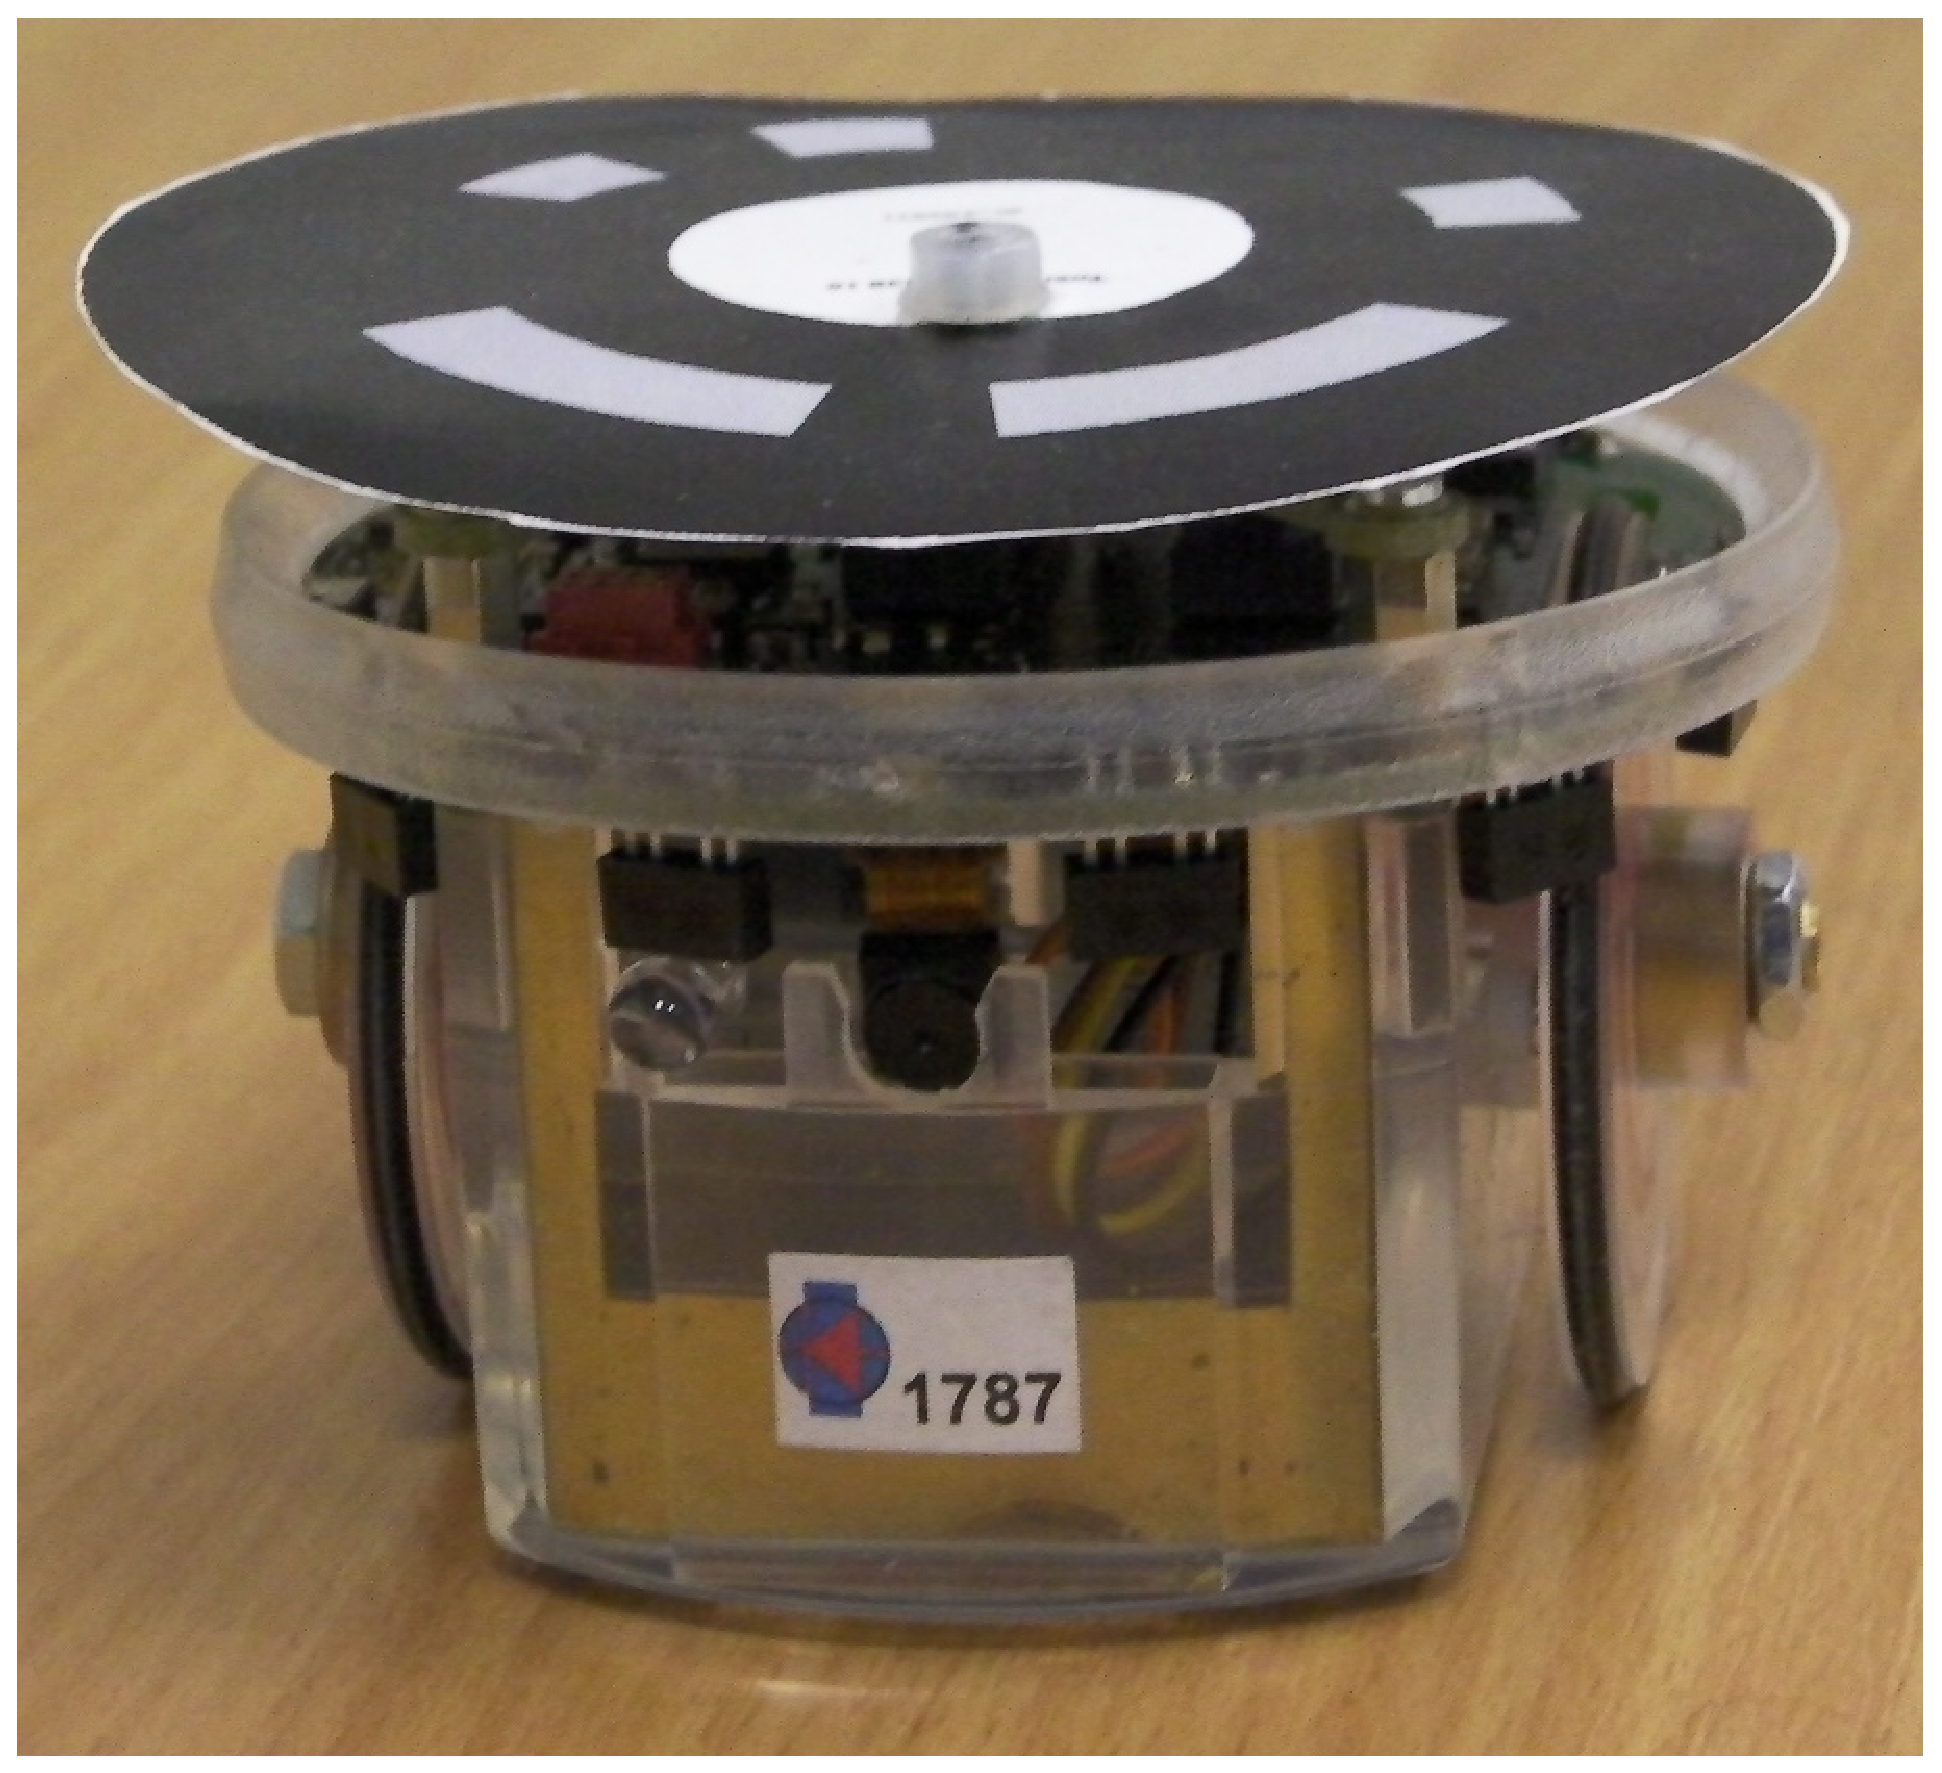
\includegraphics[width=0.3\linewidth,height=5cm]{images/epuck-happy.eps}} 
\hspace{1cm}
\subfloat[A binary-coded marker]{
\includegraphics[width=0.3\linewidth,height=5cm]{images/20-31412.eps}}
\caption{(a) The e-puck robot with SwisTrack marker on top, (b) A binary coded marker that can be tracked by an overhead camera  using SwisTrack.}
\label{fig:e-puck}
\end{figure*}
%%
\begin{figure*}
\centering
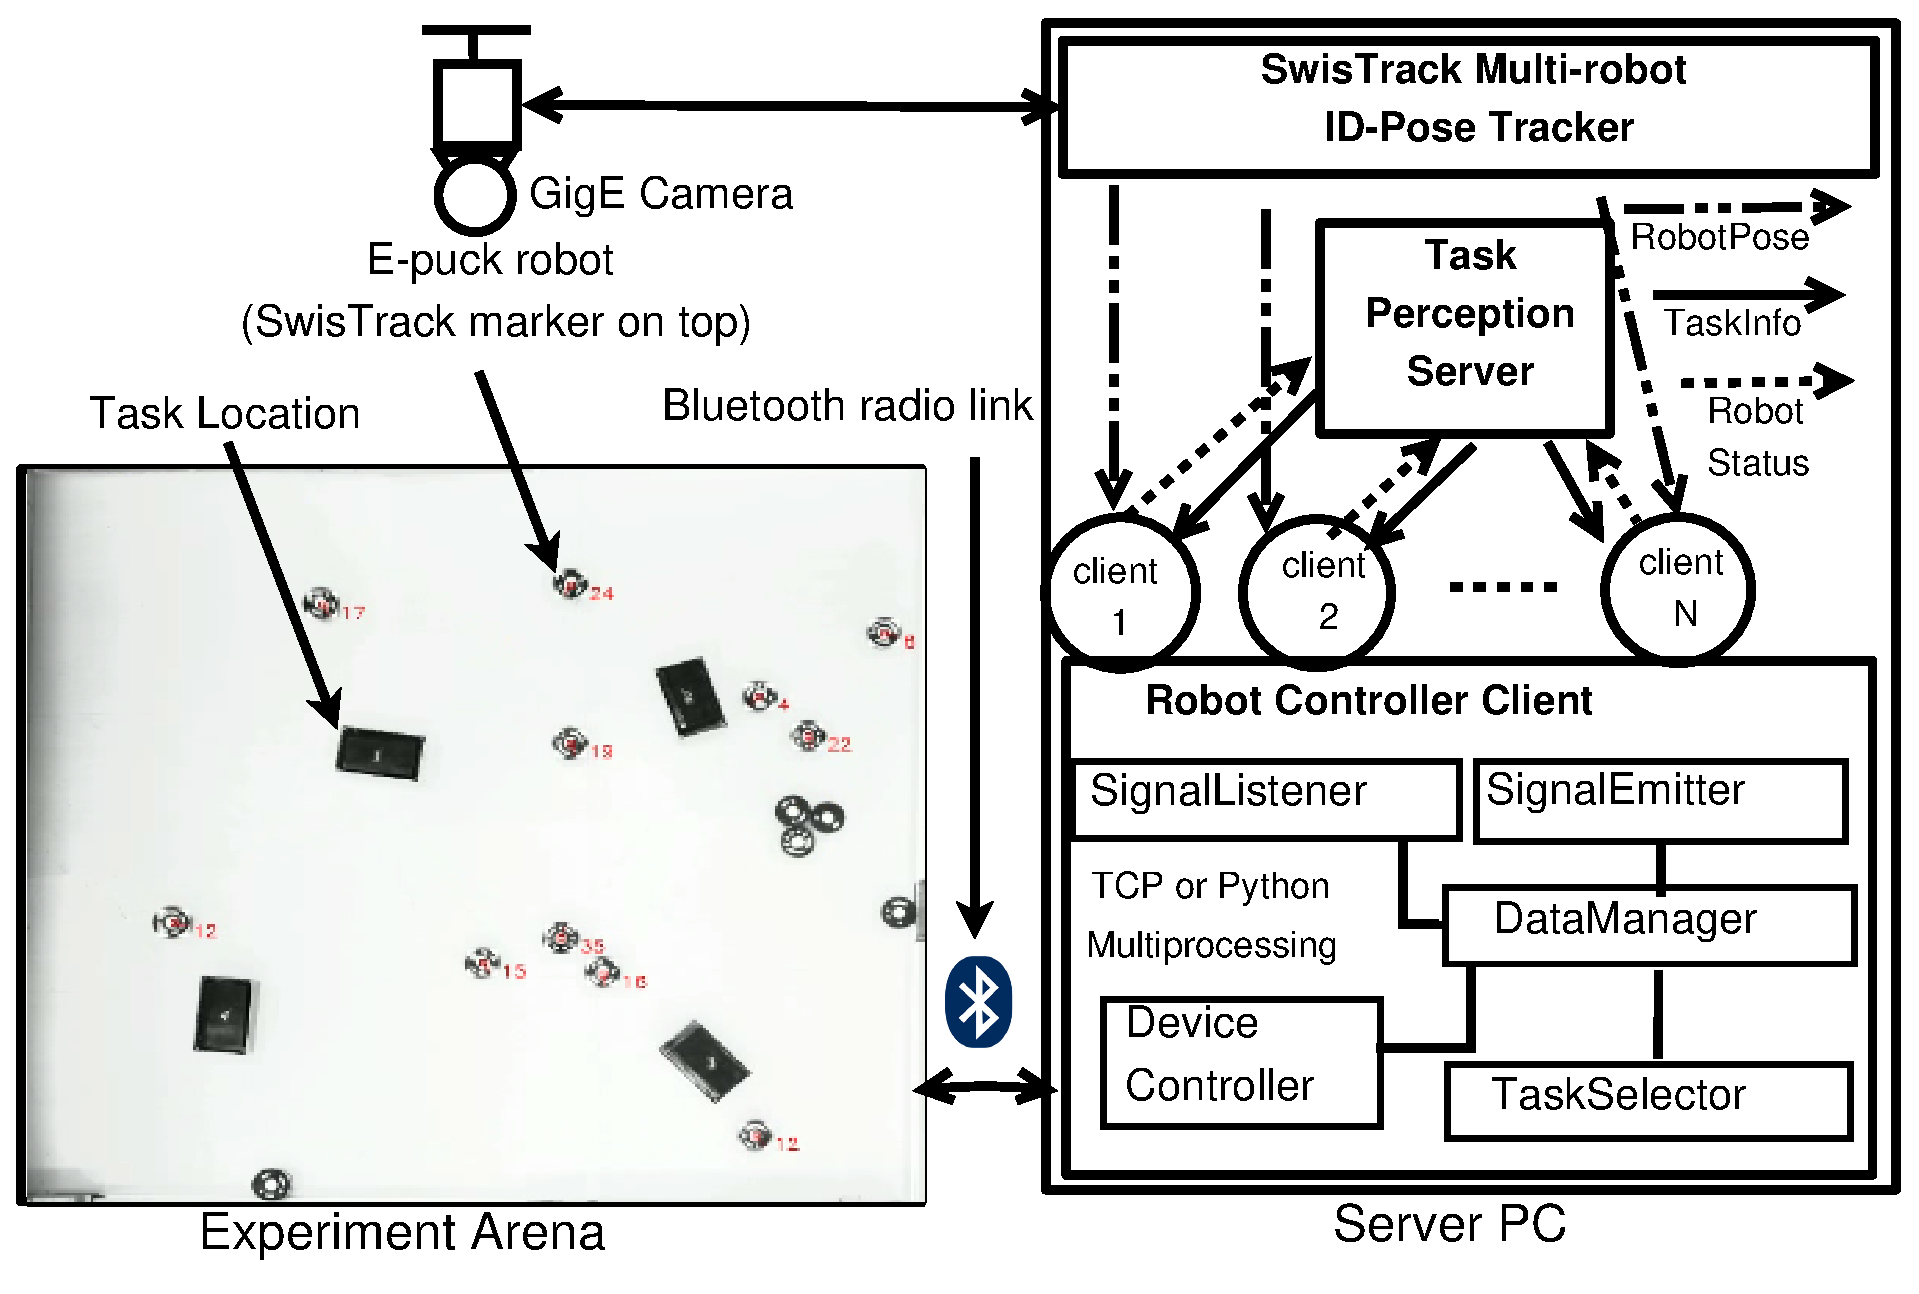
\includegraphics[width=0.9\textwidth, angle=0]
{./images/RIL-Expt-Setup1.eps}
%figure caption is below the figure
\caption{Hardware and software setup for series A \& B experiments}
\label{fig:RIL-Expt-Setup1} % Give a unique label
\end{figure*}
%%
Ideally, AFM can be implementation as a complete distributed task-allocation system where each agent selects its own task based on its own external perception about task-urgencies (i.e. attractive fields),  distances from tasks and internal task-sensitisation records. Such an implementation requires powerful robots with sophisticated sensors (camera, laser etc.) and sufficient computation and communication  capabilities. In that case, robots can keep  task-urgency information up-to-date  through suitable local communication  schemes with their peers who can monitor the tasks. By using suitable navigation and mapping modules, they can also accurately calculate the distances from tasks and navigate to tasks autonomously. Moreover, they also require necessary hardware to do the actual task, e.g. gripper for picking up objects. However, in this study, we are particularly interested to find the suitable communication schemes that can effectively spread the attractive fields (task-urgencies) among robots. So we have simplified the complexities of a full-fledged implementation by using a centralized communication system  that effectively makes up the limitations of our e-puck robots.  For example, our robots are not  capable of sensing a task to estimate its urgencies, instead our centralized TPS broadcast task information, e.g. task-urgencies, locations etc. to robots in certain time intervals. 

\begin{figure*}
\centering
\hspace*{1cm}
%\includegraphics[width=10cm,height=7.5cm,angle=0]
\subfloat[]{
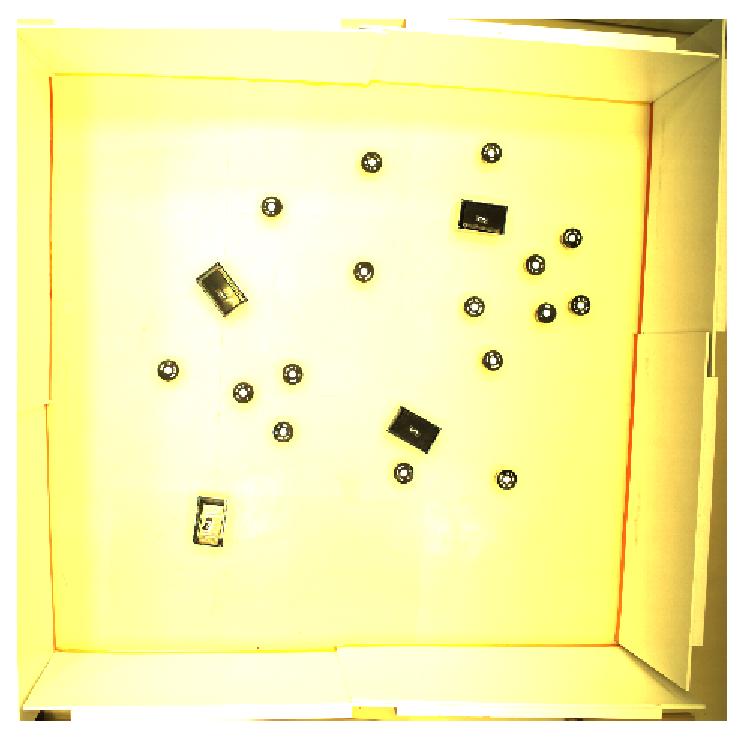
\includegraphics[width=0.65\linewidth,angle=0]
{./images/RILSnapshot1.eps}}
\newline
\subfloat[]{
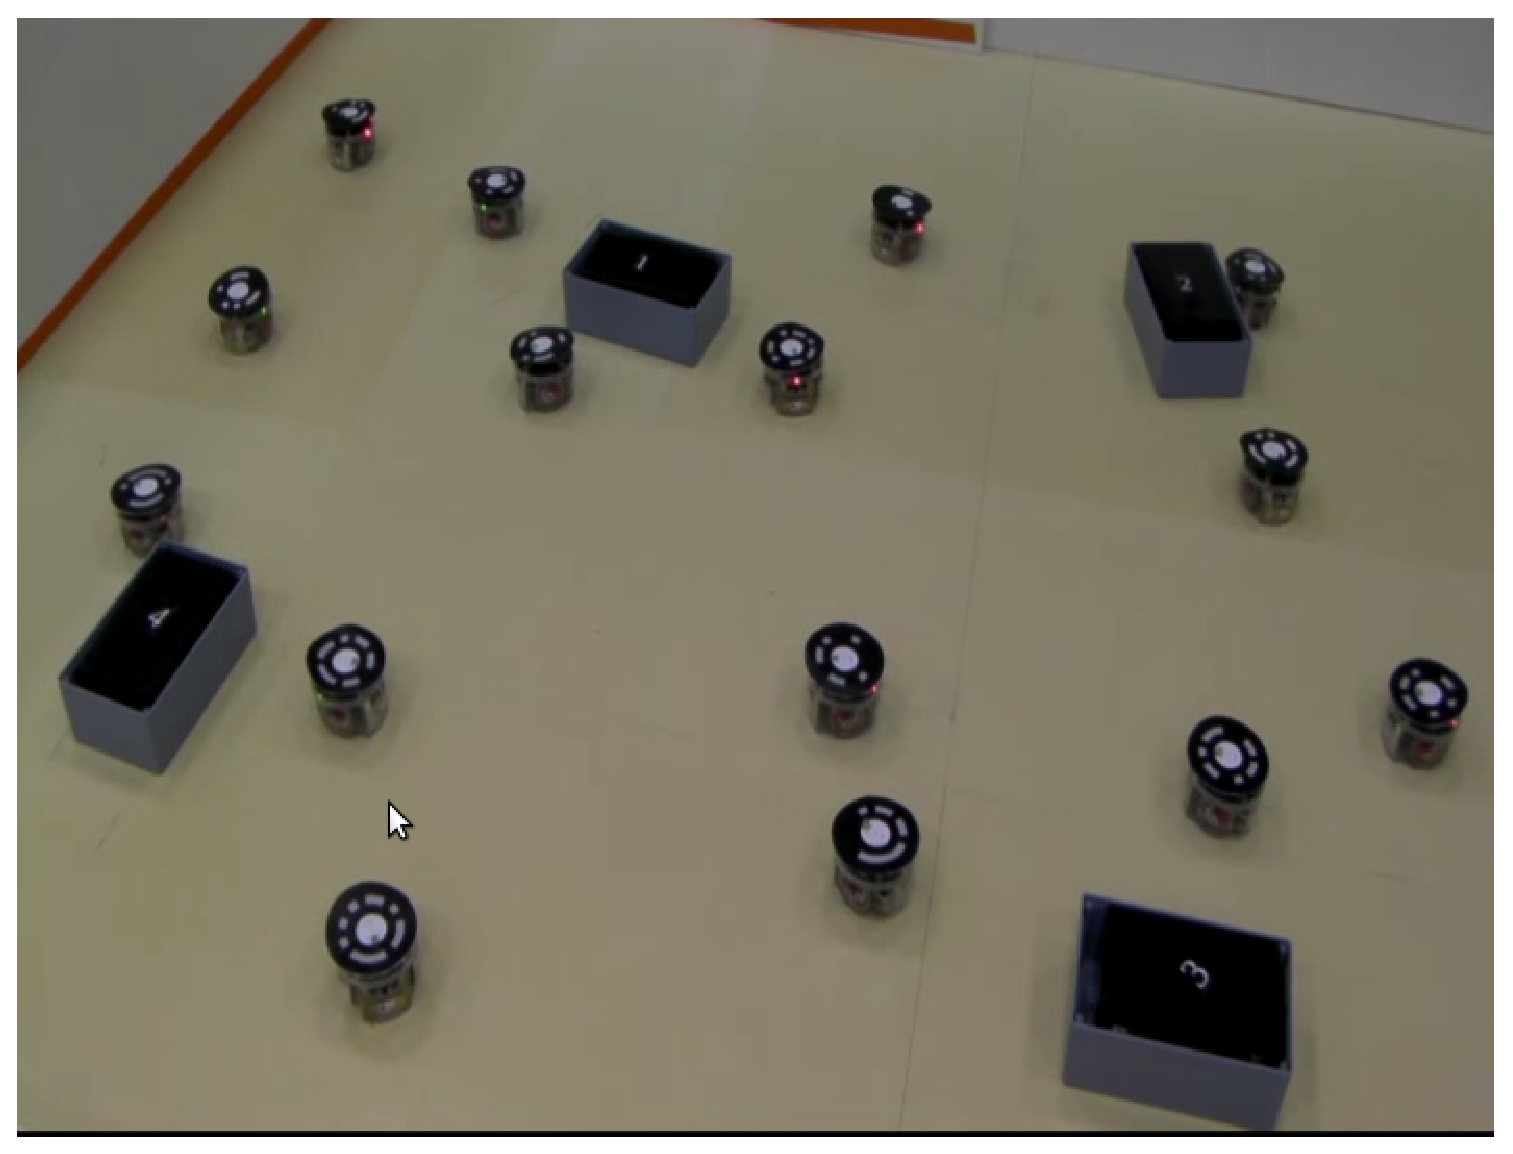
\includegraphics[width=0.65\linewidth]
{./images/RILCamcorderSnapshot1.eps}}
\caption{Our experiment arena captured by (a) a GigE4900C camera mounted on 3m high ceiling (b) an ordinary camcorder.}
\label{fig:expt-arena} % Give a unique label
\end{figure*}
%%
In our current implementation, instead of doing any real work with powerful robots, we emulate a mock manufacturing shop-floor scenario that requires the robot only to travel among tasks. As our robots do not have on-board CPU, they need a host PC to  control them using BTCom Bluetooth communication protocol over the wireless link \cite{Mondada+2009}. Thus our host-PC runs one RCC for each physical robot. These RCCs also rely upon SwisTrack multi-robot tracking system for updating their real-time pose. So although our MRTA solution is distributed by design, we primarily used a centralized approach to implement it due to the limitations of our robots and the convenience of implementation. Table \ref{table:dbus-signals} list the D-Bus communication interfaces among our software components. Fig. \ref{fig:concrete-arch} outlines the placements of various software components of our multi-robot control architecture based on their functional characteristics and processing requirements \cite{Sarker2010control}.
%%
\begin{table*}
\caption{D-Bus signal interfaces among software components.}
\label{table:dbus-signals}
\begin{center}
\begin{tabular}{|l|l|l|p{1.8in}|p{0.5in}|}
\hline D-Bus Signal &  Source & Destination  & Payload & Used in\\ 
\hline RobotPose & SwisTrack & RCC  & Robot-pose x, y and oientation theta. & GSNC \& LSLC\\ 
\hline TaskInfo & TPS & RCC & An array of all tasks' information each of them contains: task-id, time-stamp, task pose (x,y), task-urgency. & ,, \\ 
\hline RobotStatus & RCC & TPS & Robot's id and its currently executing task's id. & ,, \\ 
\hline RobotPeers & SwisTrack & RCC & List of IDs of peers of each robot within its communication range. & LSLC \\ 
\hline TaskNeighbour & SwisTrack & TPS &  List of IDs of robots that are co-located within a task's perception range. & ,,\\ 
\hline LocalTaskInfo & RCC & RCC & An array of known tasks' information. & ,,\\
\hline 
\end{tabular}
\end{center} 
\end{table*}
%%
\begin{figure*}
\begin{center}
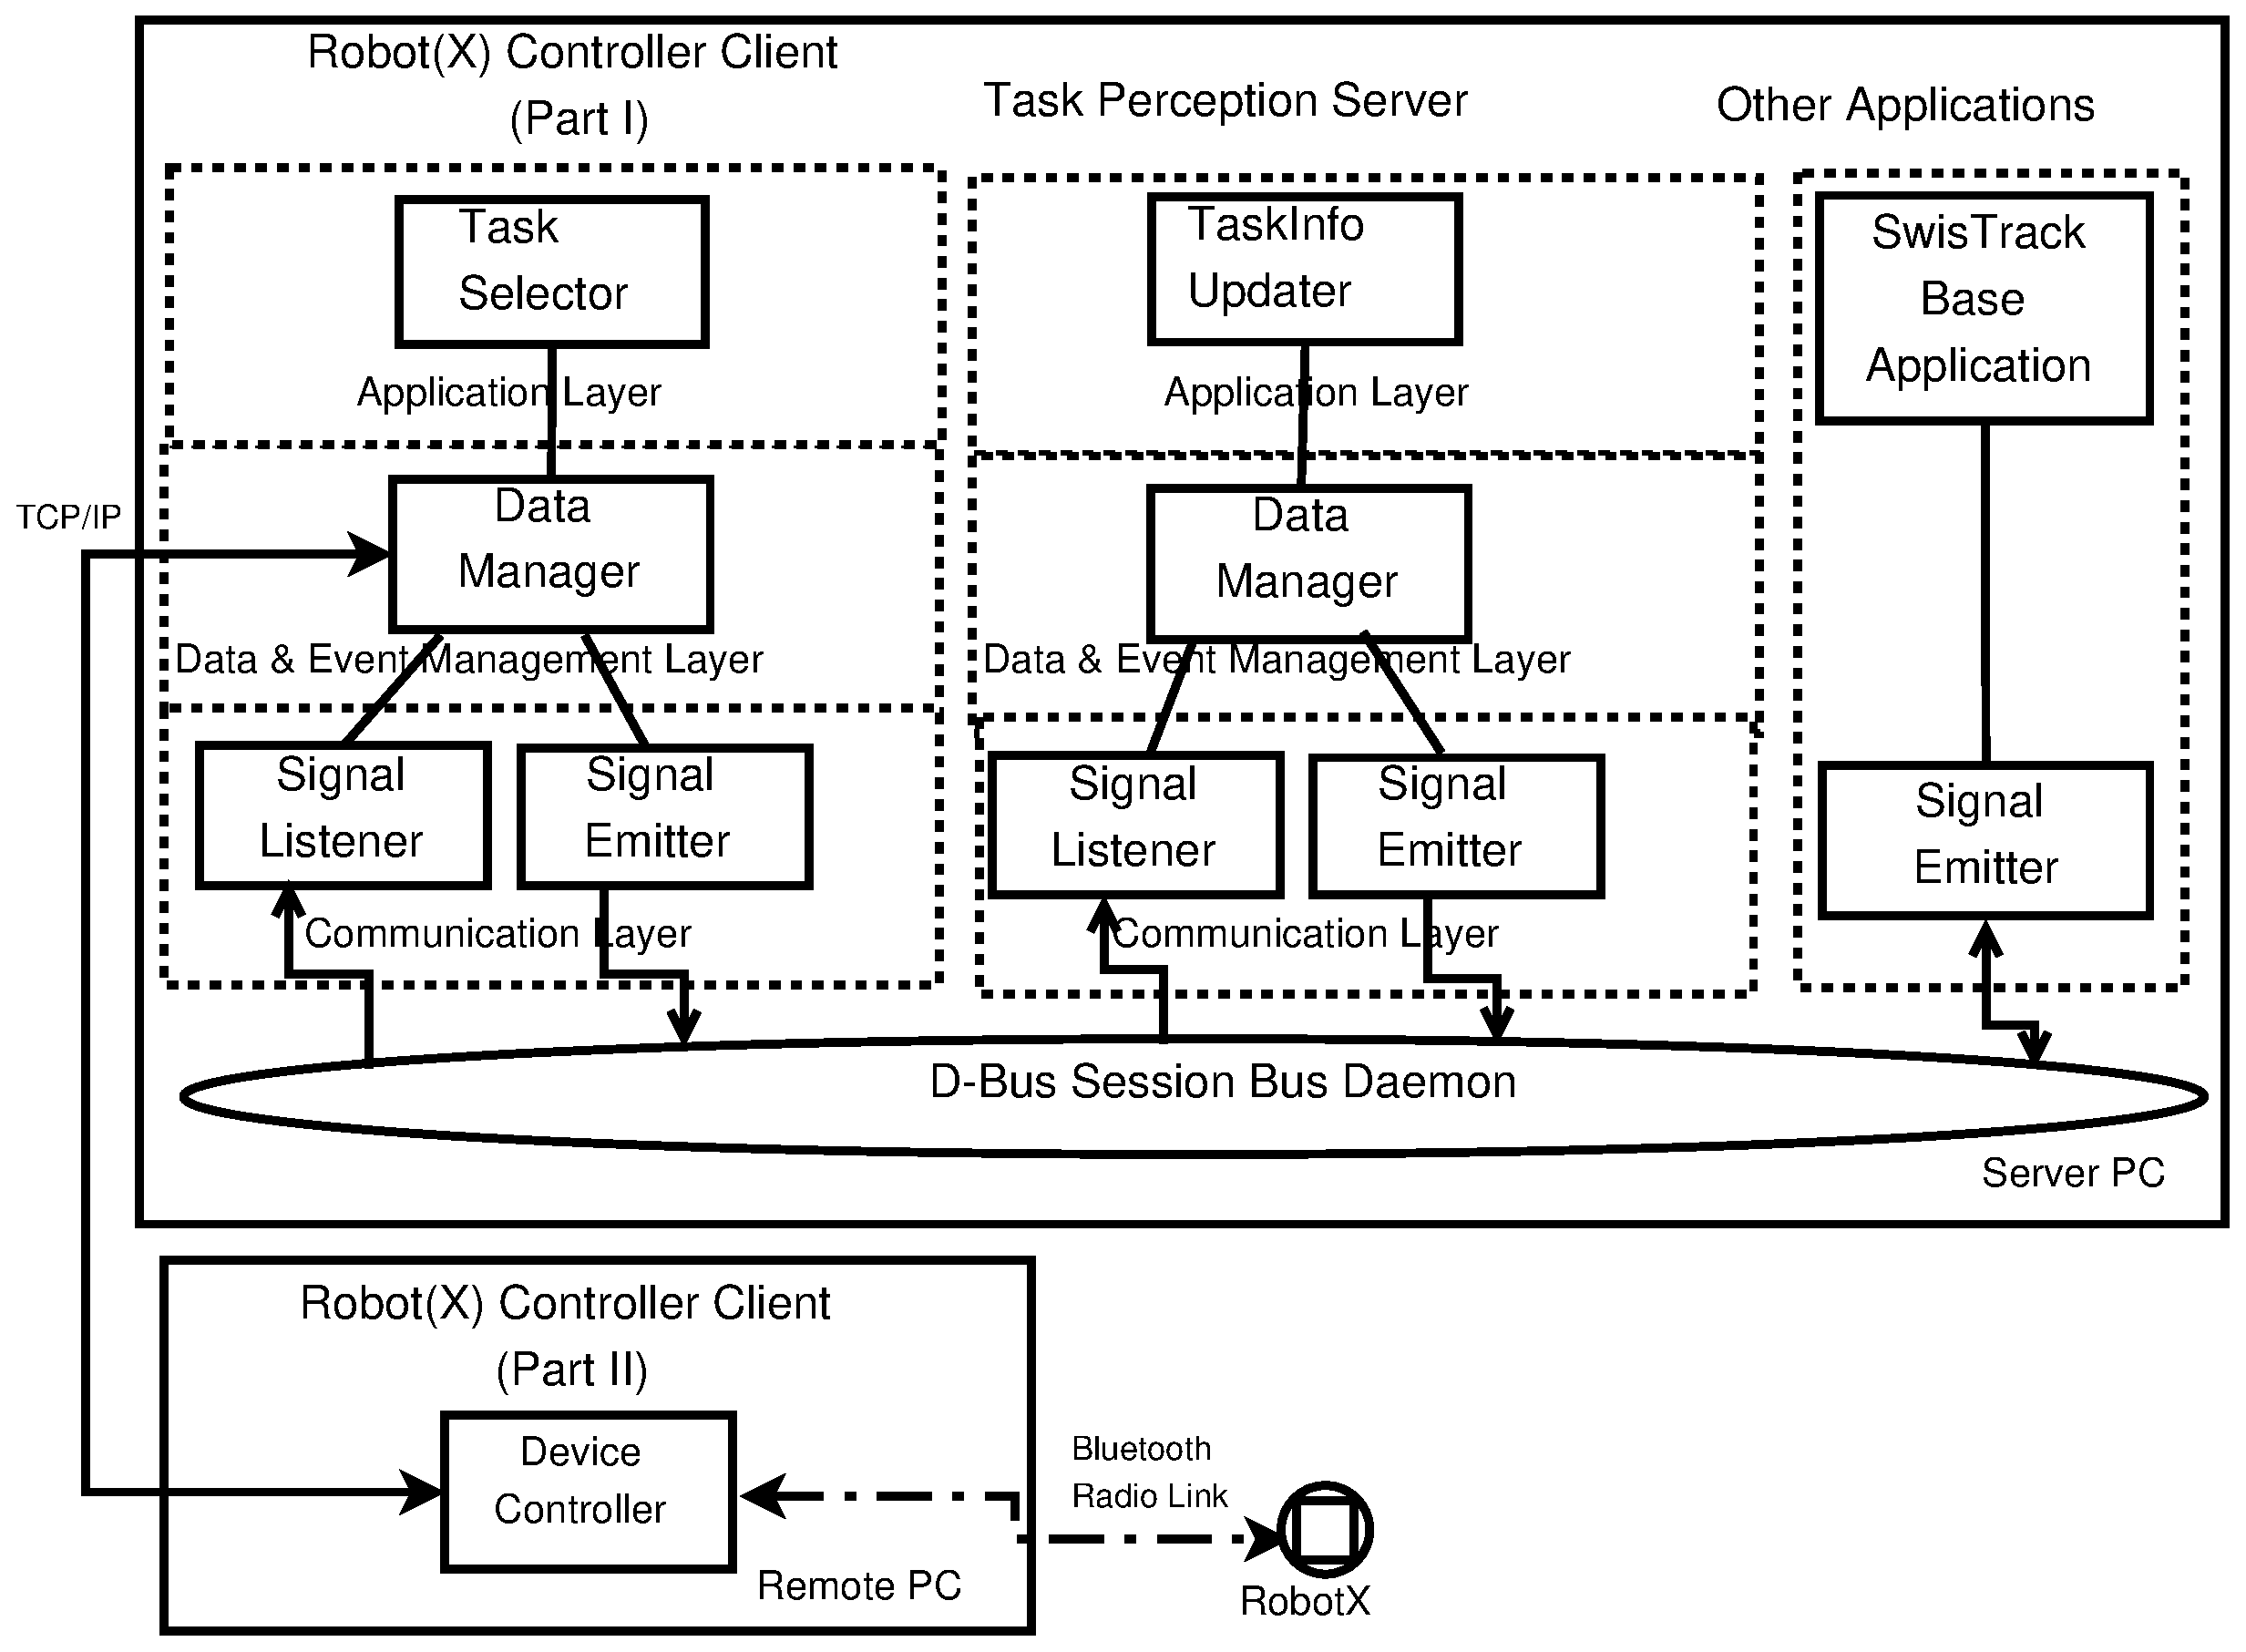
\includegraphics[width=0.7\linewidth,height=10cm]{./images/concrete-arch} 
%\centering
\caption{General outline of {\em HEAD}. A RCC application has been split into two parts: one runs locally in server PC and another runs remotely, e.g., in an embedded PC.} 
\label{fig:concrete-arch}
\end{center}
\end{figure*}
%%
\begin{figure*}
\centering
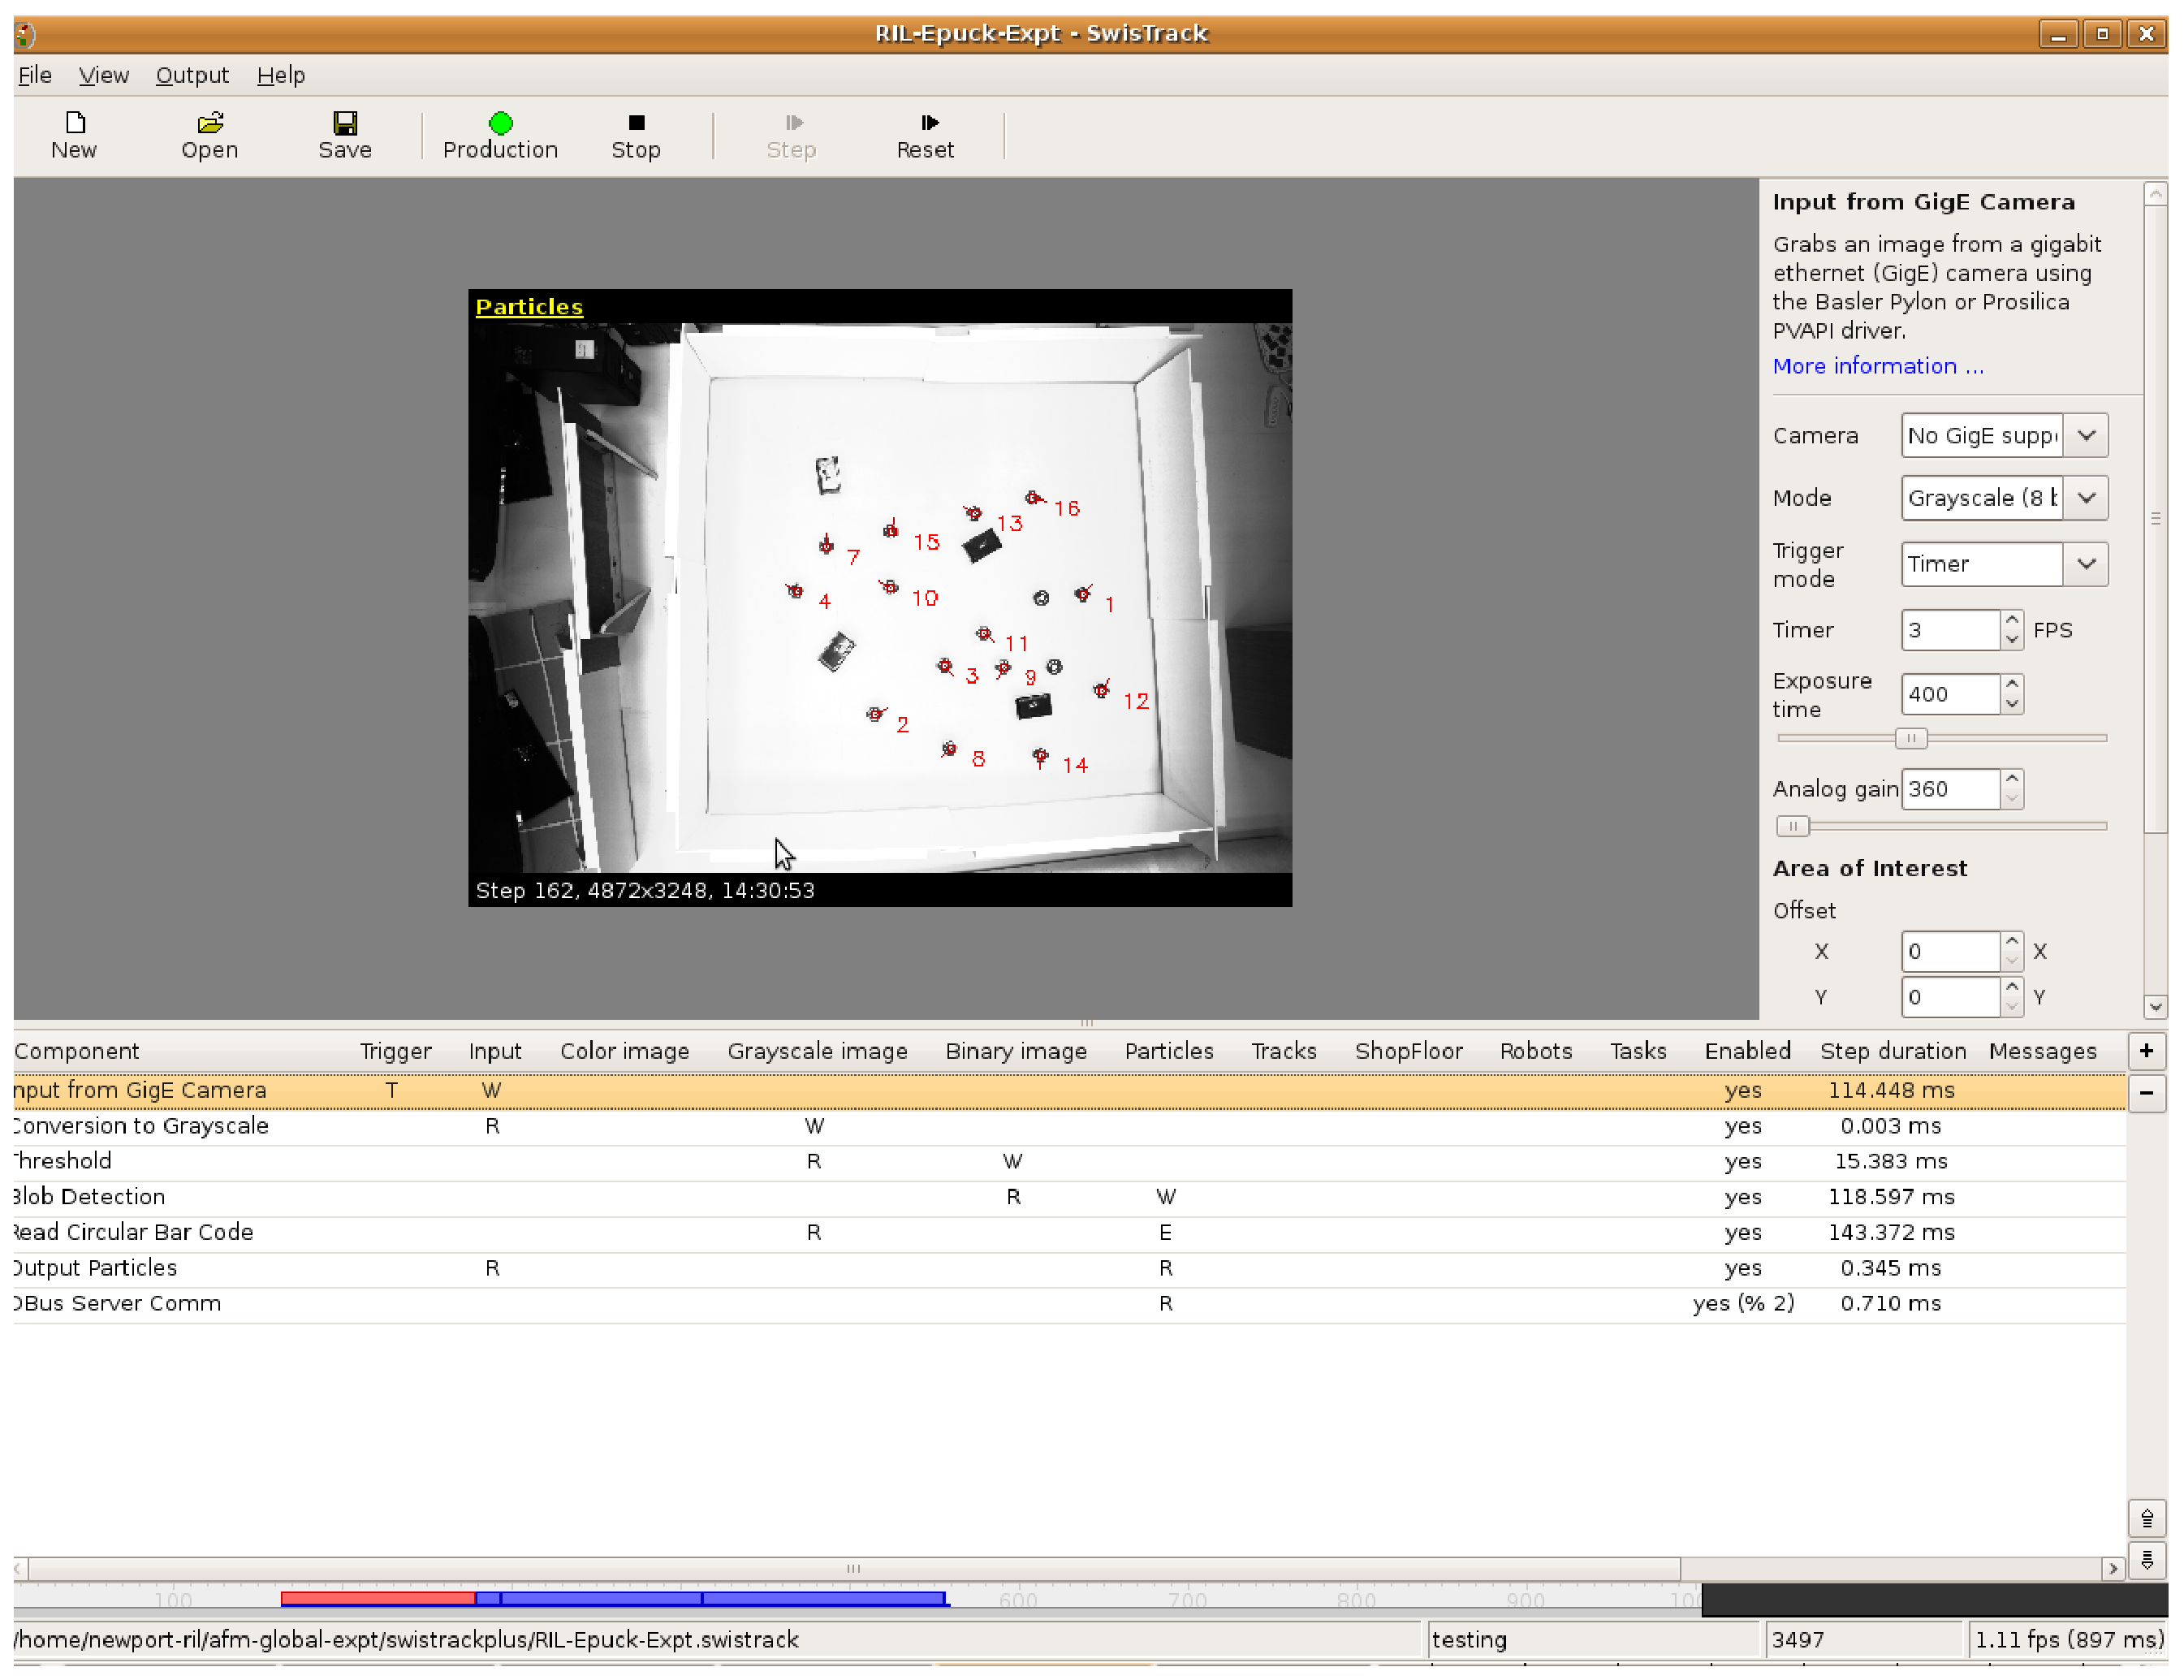
\includegraphics[width=0.7\linewidth,height=10cm]
{./images/SwisTrackScreenshot.eps}
\caption{SwisTrack tracking a team of 16 robots under Ubuntu Linux 9.10 OS.}
\label{fig:swistrack-screenshot} 
\end{figure*}
%-----------------------
\subsubsection{RCC Modules}
As shown in Fig. \ref{fig:RIL-Expt-Setup1}, each e-puck robot is controlled by a corresponding RCC. A RCC sends commands to the robot's firmware using BTCom protocol. A RCC consists of several Python modules. Each module represents a sub-process under a main process that ties all of them together by using Python's Multiprocessing module\footnote{http://docs.python.org/library/multiprocessing.html}. Below we have described briefly the implementation of these Python modules. All code are publicly accessible through GitHub repository\footnote{git://@github.com/roboshepherd/EpuckCentralizedClient.git,    
\textit{hash:}7e3af8902e64db3fa59e}.
%%
%%
\begin{table}
\caption{Data structures and events used by the RCC}
\begin{center}
\begin{tabular}{|l|l|}
\hline \textbf{Data structure} & \textbf{Related event(s)}\\ 
\hline \texttt{\texttt{mRobotID}} & - \\ 
\hline \texttt{mRobotPose} & \texttt{mRobotPoseAvailable}\\ 
\hline \texttt{mTaskInfo} & \texttt{mTaskInfoAvailable}\\ 
\hline \texttt{mSelectedTask} & \texttt{mSelectedTaskAvailable}\\
 &  \texttt{mSelectedTaskStarted}\\
 &  \texttt{mTaskTimedOut}\\
 \hline 
\end{tabular}
\end{center}
\label{table:data-mgr}
\end{table} 
%---------------------
In the implementation of RCC, we have employed a data and event management process called \texttt{DataManager} that acts as a data warehouse and event management centre for RCC. Table \ref{table:data-mgr} list the major data structures and corresponding event channels of \texttt{Data Manager}. Here \texttt{mRobotID} represents the e-puck robot's marker ID (converted to decimal number from the binary code) which uniquely identifies a robot from others.  We have used Python {\em dictionary} type data structure for all other data structures that are managed by the Python Multiprocessing's {\em Manager()} object.  \texttt{DataManager} object also runs a tiny TCP/IP server process powered by the Multiprocessing's {\em RemoteManager()} interface. So, if necessary,  any other process can access all of the DataManger's data structures and event channels remotely by instantiating a proxy client  that connects to this TCP/IP server process.

We have employed two D-Bus communication modules in RCC: \texttt{SignalListener} and \texttt{SignalEmitter}, that are responsible for listening and emitting D-Bus signals respectively. \texttt{SignalListener}, has subscribed to D-Bus session bus for listening  to D-Bus \texttt{RobotPose} and \texttt{TaskInfo} signals. \texttt{SignalEmitter} makes use of Python {\em sched} module that enables it to check periodically \texttt{mSelectedTaskStarted} event and emit a robot's task status containing signal, \texttt{RobotStatus}. \texttt{TaskSelector} works in the application layer of our multi-robot control architecture. It plugs the AFM algorithms (Sec. \ref{ss:rcc-alg}) into RCC to select task based-on \texttt{DataManger}'s event notifications.
%%
\begin{figure*}
\centering
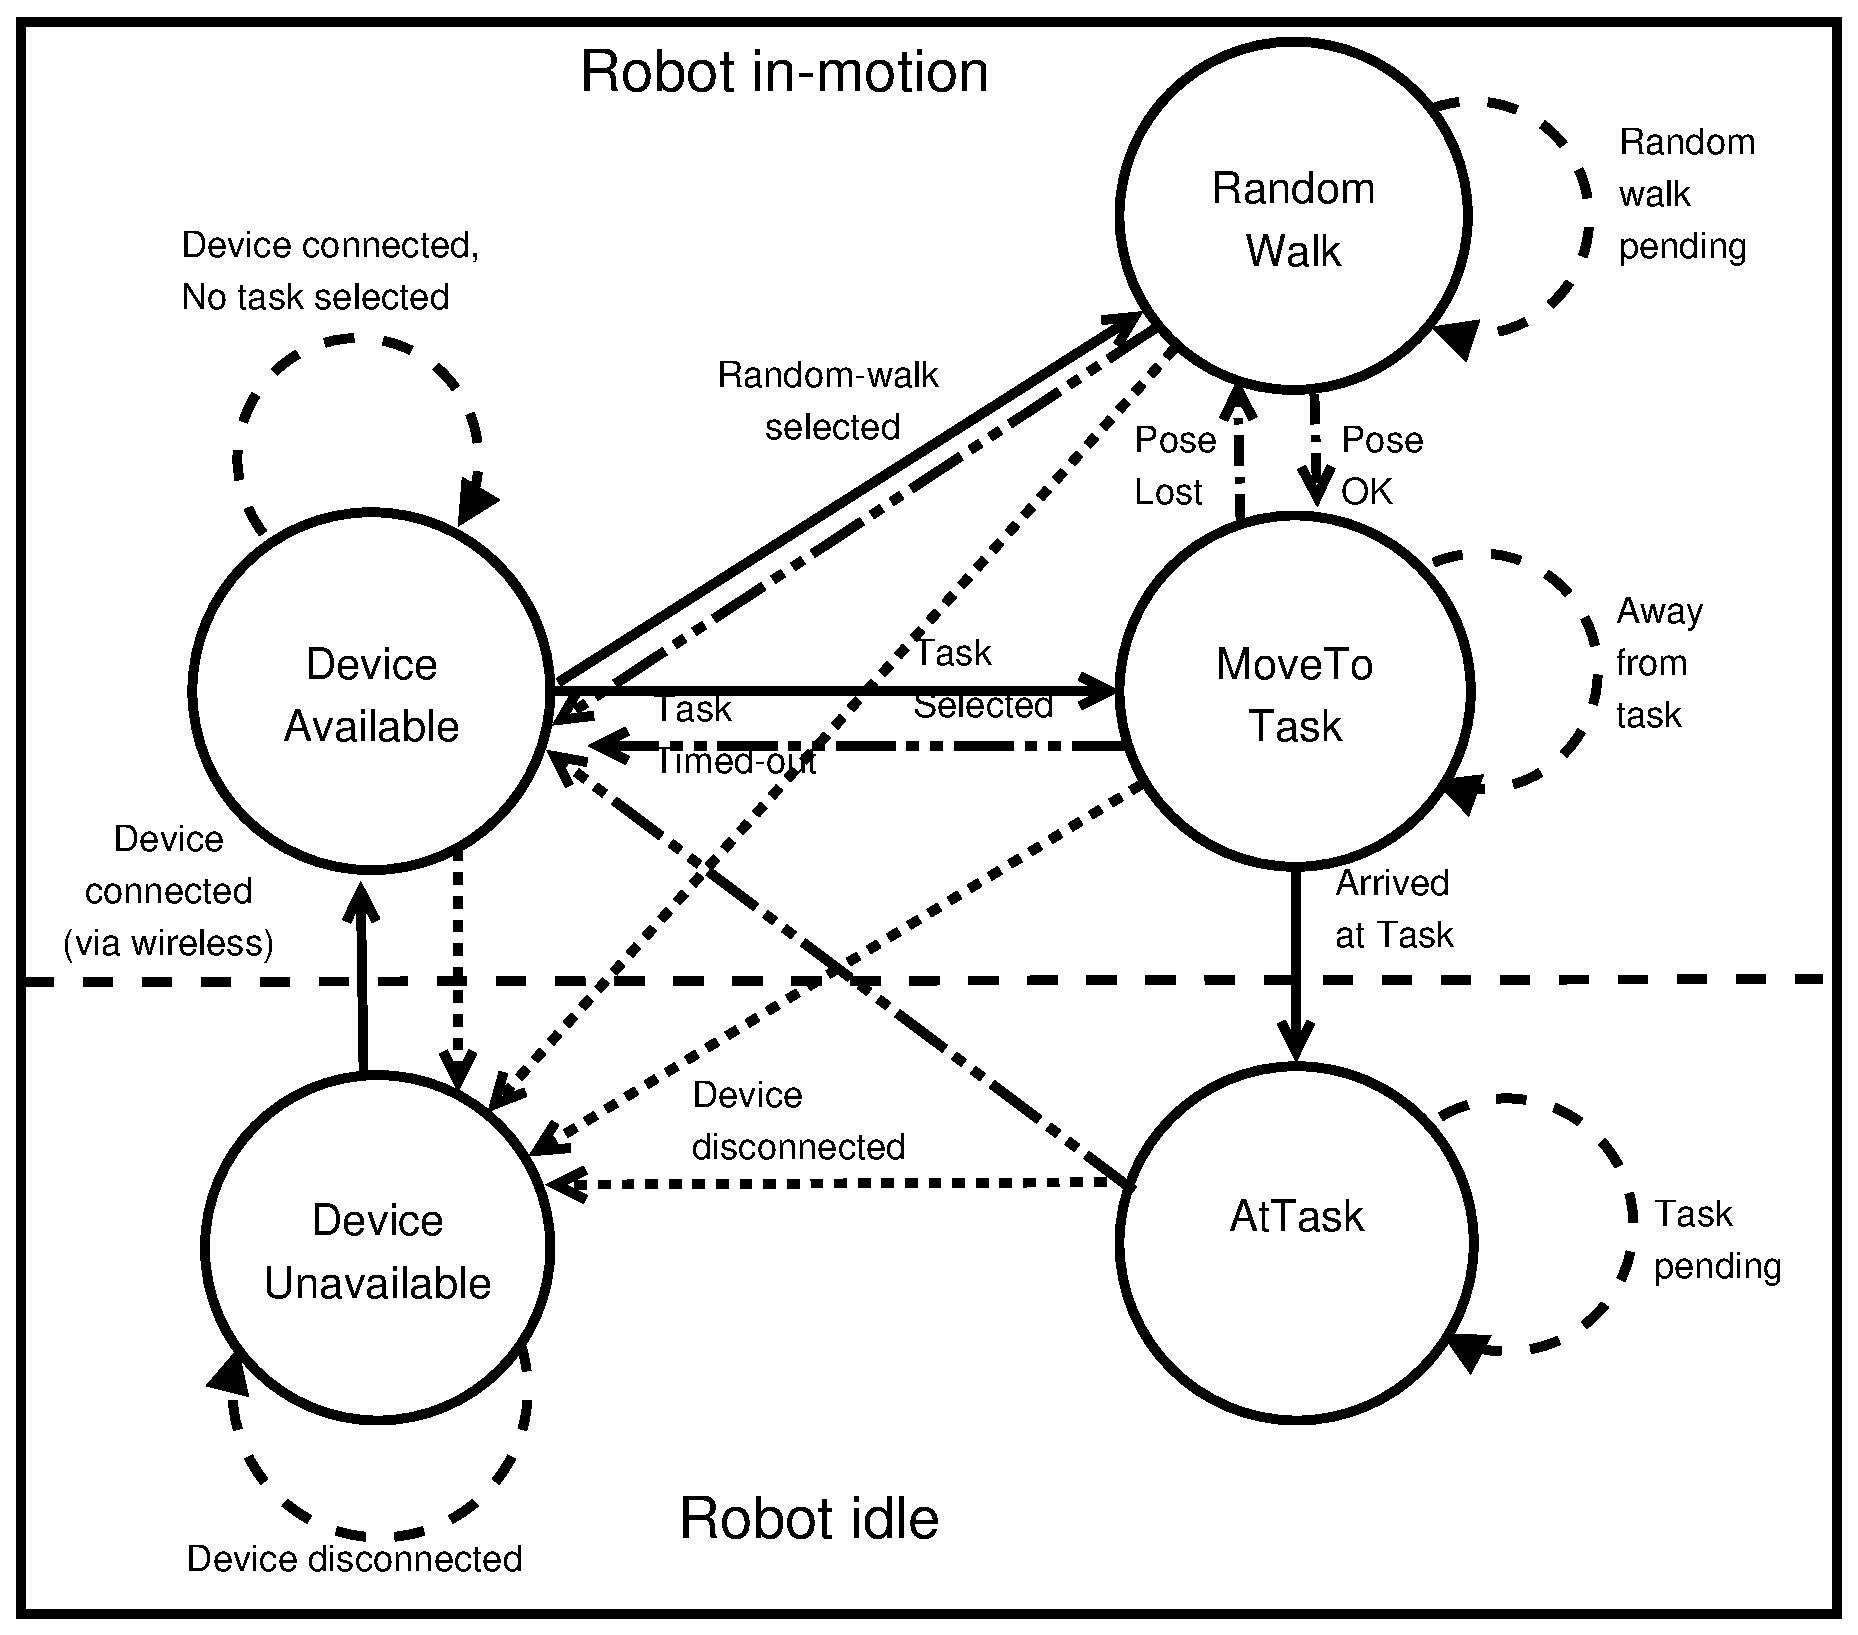
\includegraphics[width=0.7\linewidth,height=11cm]
{./images/rcc-device-controller-state.eps}
%figure caption is below the figure
\caption{State diagram of \texttt{DeviceController} module}
\label{fig:dc-states} % Give a unique label
\end{figure*}

The final code that moves a robot to desired task location or make random-walk resides in \texttt{DeviceController} module. When \texttt{TaskSelector} sets  \texttt{mSelectedTaskAvailable} event \texttt{DeviceController} sub-process checks the Bluetooth link-connectivity with physical robot. In case of successful task start-up it sets \texttt{mSelectedTaskStarted} event that, in turn, triggers \texttt{SignalEmitter} to emit a D-Bus signal publishing the robot's currently engaged task. The full state switching policies of \texttt{DeviceController} is illustrated in Fig. \ref{fig:dc-states}. Externally we can observe two distinct physical state of a robot: it is either idle or in motion (separated by dotted line). These two physical states are mapped into several logical steps as described below.

\textbf{DeviceUnavailable: }
Periodically \texttt{DeviceController} checks whether the device has connected to host-PC and changes its state to \textit{DeviceAvailable} (i.e device connected). We can see that from every other state, device can come to this unavailable state (shown by dotted arrow) when the  link is lost e.g. in case of robot's low battery or any other disconnection event (i.e device disconnected).

\textbf{DeviceAvailable: }
\texttt{DeviceController} stays in this state until \texttt{Data-Manager}'s mSelectedTaskAvailable event fires (Device connected, no task selected). Then it switches to either \textit{MoveToTask} or \textit{RandomWalk} state depending on the selected task.  \texttt{DeviceController}  returns to this state from \textit{RandomWalk}, \textit{MoveToTask} or \textit{AtTask} states after a pre-set task time-out period has elapsed.  In that case it triggers the \texttt{DataManager}'s \texttt{mTaskTimedOut} event.

\textbf{RandomWalk: }
Robot can random walk in two cases: 1) when \texttt{TaskSelector} selects this random-walk task or 2) when the robot can not get its pose information for a moment. The latter helps the pose tracker to recover the robot-pose from a crowd of robots. Robot continues to do random-walk until it's task time-out period elapses or it's pose remains unavailable from the pose tracker (i.e. random-walk pending).

\textbf{MoveToTask: }
In this state, robot takes step-by-step navigation approach to reach a task boundary. Until the robot reaches the task boundary (Away from task), in every navigation-step it adjusts its heading to task based on both  robot and task pose information and then makes a fixed-time translation movement. In worse cases, when time-out happens early before reaching a task  \texttt{DeviceController} switches from this state to \textit{DeviceAvailable} state. However, if the same task is selected immediately, it is more likely that it will go to \textit{AtTask} state in next few steps.

\textbf{AtTask: }
In this state  \texttt{DeviceController} discovers itself neat the task and normally until task time-out happens (i.e. task pending) it stays at this state.

In order to realize LPCM strategy, in the implementation of RCC we have added three new D-Bus signal interfaces. They are briefly specified in Table \ref{table:dbus-signals}. Our base implementation of RCC's task-allocation (i.e. \texttt{TaskSelector}) is almost unchanged in this local implementation. The only thing we need to extend is the D-Bus signal reception and emission interfaces that catches the above signals and put the signal payload in \texttt{DataManager}. For the sake of simplicity, we have merges the perceived \texttt{TaskInfo} with communicated \texttt{LocalTaskInfo} into one so that \texttt{TaskAllocator} always gets all available task information. We have not made any major change in other modules of RCC, i.e. \texttt{DeviceController}. The full Python implementation of this RCC is available for download from the GitHub repository\footnote{http://github.com/roboshepherd/EpuckDistributedClient }.
%---------------------------
\subsubsection{TPS modules}
In our GSNC strategy based implementation of TPS periodically broadcasts \texttt{TaskInfo} signals to all robots using similar D-Bus signal emitting and listening modules. Task information has been updated by a separate Python module following the TPS algorithm described before. In the local version, TPS only emits \texttt{TaskInfo} signal when a robot is within a task's perception range, $r_{task}$ based-on the \texttt{TaskNeighbour} signal from SwisTrack. For this additional interface, we have extended D-Bus \texttt{SignalListener} to catch this additional D-Bus signal.  No major changes are done in the other parts of TPS implementation. The full Python implementation of TPS is available for download from the authors' GitHub centralized\footnote{http://github.com/roboshepherd/CentralizedTaskServer}
and distribued \footnote{http://github.com/roboshepherd/DitributedTaskServer} repositories.
%%==================================================================
\section{Results}
\label{sec:res}
%%
In this section we have presented our experimental results. We ran those experiments for about 40 minutes duration.  They are averaged over five iterations for Series A and B experiments and three iterations for Series C and D experiments. 
%%-------------------------------------------------
\subsection{Shop-floor work-load history}
In our experiments we have defined shop-floor work-load in terms of task urgencies. For example, Eq. \ref{eqn:task-urgency-prod-init} shows how we have calculated initial production work-load of our manufacturing shop-floor scenario. Fig. \ref{fig:raw-urgencies}  show the dynamic changes in task-urgencies for the single iteration of each experiment. The fluctuations in these plots are resulted from the different levels of task-performance of our robots. In case of Series D, we can see that an unattended task, \textit{Task4}, was not served by any robot for a long period and later it was picked up by some of the robots. 
%%
\begin{figure} 
\centering
\subfloat[Series A]
{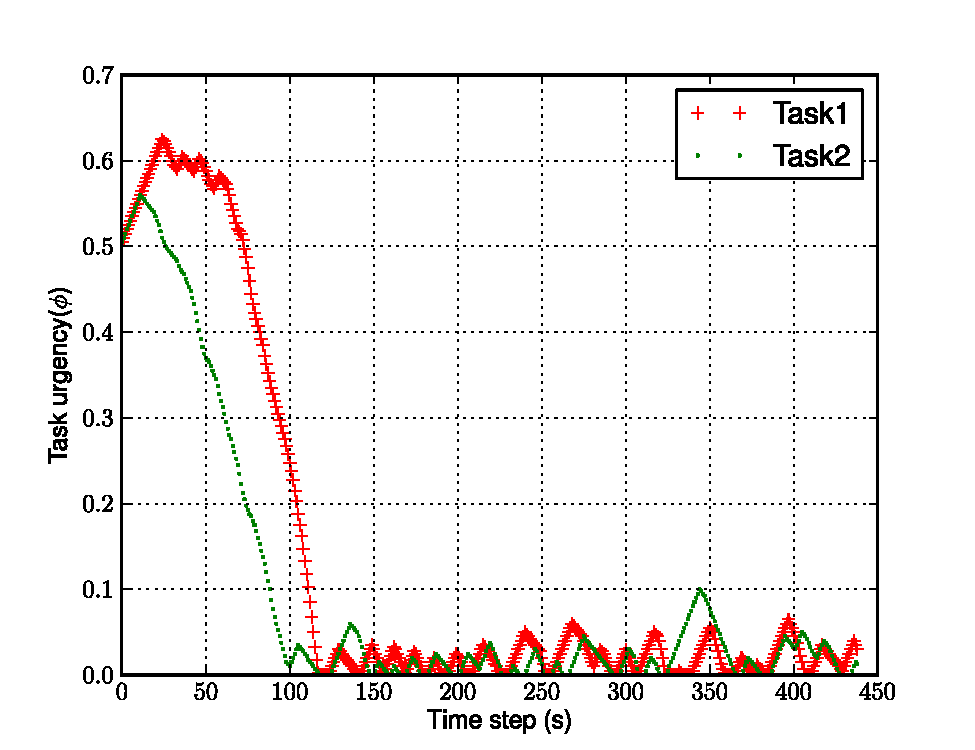
\includegraphics[width=0.7\linewidth, angle=0]
{images/SA-PlotUrgencyLog-2010Apr30-095755.eps}}
\newline
\subfloat[Series B]
{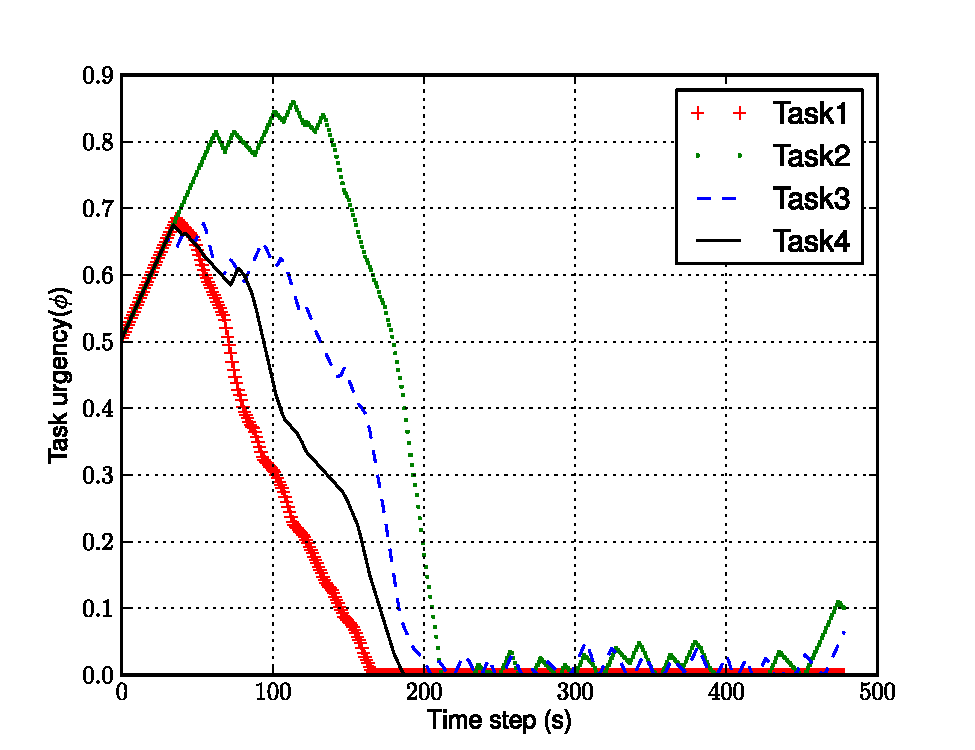
\includegraphics[width=0.7\linewidth, angle=0]
{images/SB-PlotUrgencyLog-2010May10-115549.eps}}
\newline
\subfloat[Series C]
{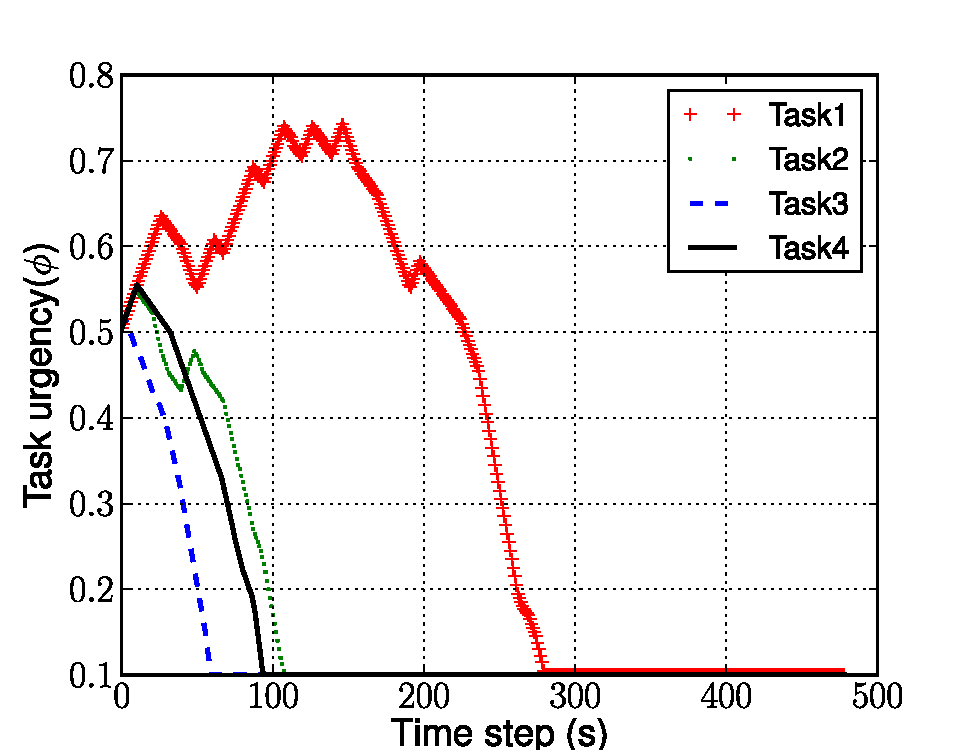
\includegraphics[width=0.7\linewidth, angle=0]
{images/SC-PlotUrgencyLog-2010Feb15-171017.eps}}
\newline
\subfloat[Series D]
{\includegraphics[width=0.7\linewidth, angle=0]
{images/SD-PlotUrgencyLog-2010Feb17-112141.eps}}
\newline
\caption{Changes in task-urgencies.}
\label{fig:raw-urgencies}
\end{figure}
%%
In order to measure the task-related work-loads on our system we have summed up the changes in all task-urgencies over time. We call this as {\em shop-floor work-load history} and formalized as follows. Let $ \phi_{j, q}$ be the urgency of a task $j$ at $q^{th}$ step and $\phi_{j, q+1}$ be the task urgency of $(q+1)^{th}$ step. We can calculate the sum of changes in urgencies of all $M$ tasks at $(q+1)^{th}$ step:
\begin{equation} 
\Delta \Phi_{j, q+1} = \sum_{j=1}^{M} (\phi_{j, q+1} - \phi_{j, q})
\label{eqn:Delta-Phi}
\end{equation}
Fig. \ref{fig:urgency-stat} shows the dynamic shop-floor workload for all four series of experiments. From these plots, we can see that initially the sum of changes of task urgencies (shop-floor workload) is going towards negative direction. This implies that tasks are being served by a high number of robots. 
%%
\begin{figure}
\centering
\subfloat[Series A]
{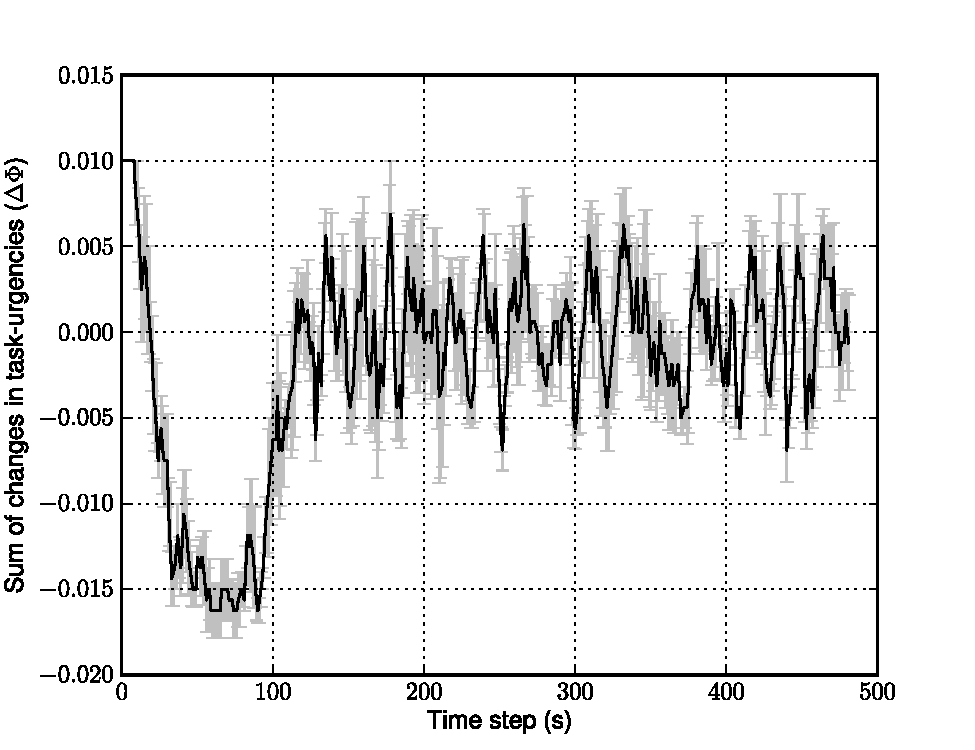
\includegraphics[width=0.7\linewidth, angle=0]
{images/SA-8robots2tasks-TaskUrgencyStat.eps}}
\newline
\subfloat[Series B]
{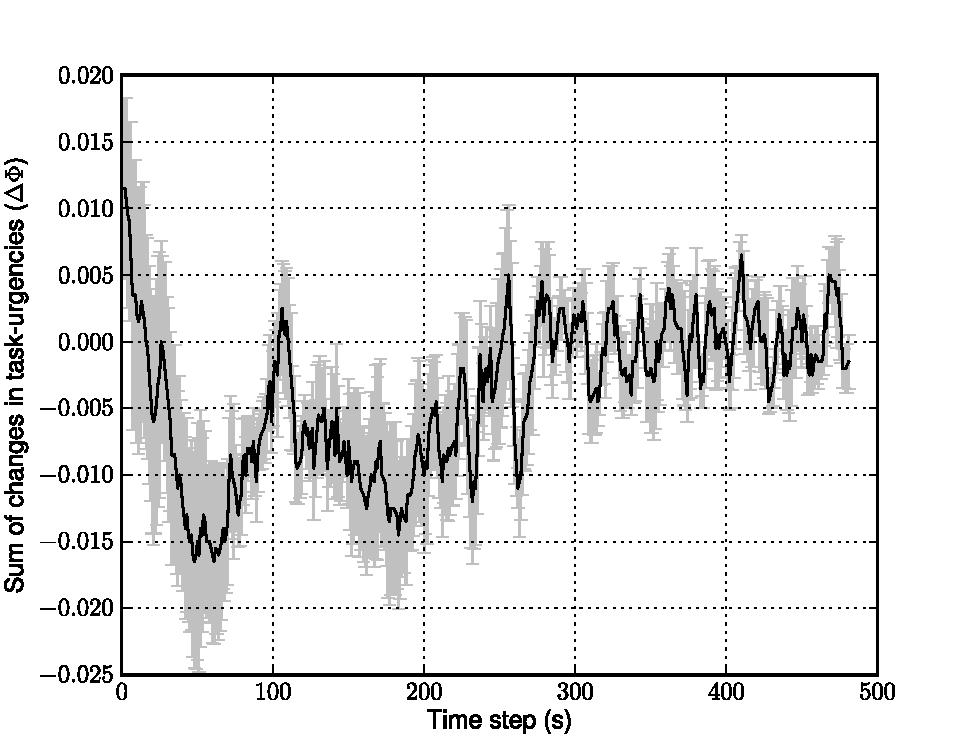
\includegraphics[width=0.7\linewidth, angle=0]
{images/SB-TaskUrgencyStat.eps}}
\newline
\subfloat[Series C]
{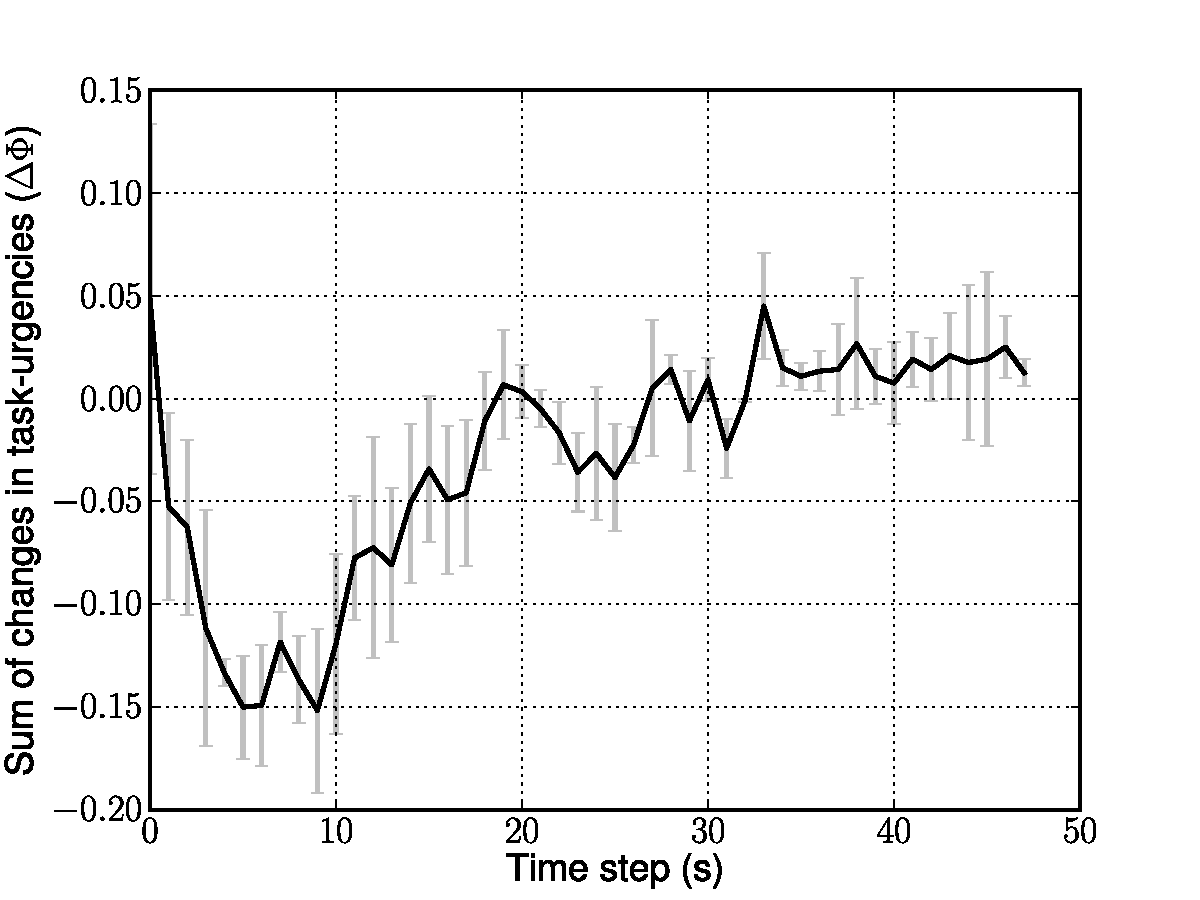
\includegraphics[width=0.7\linewidth, angle=0]
{images/SC-TaskUrgencyStat.eps}}
\newline
\subfloat[Series D]
{\includegraphics[width=0.7\linewidth, angle=0]
{images/SD-TaskUrgencyStat.eps}}
\newline
\caption{Shop-floor workload change history.}
\label{fig:urgency-stat}
\end{figure}
%%
%%----------------------------------------------------------------
\subsection{Ratio of active workers}
%%
\begin{figure}
\centering
\subfloat[Series A]
{\includegraphics[width=0.7\linewidth, angle=0]
{images/SA-Plasticity-8robots2tasks.eps}}
%\hspace{0.2cm}
\newline
\subfloat[Series B]
{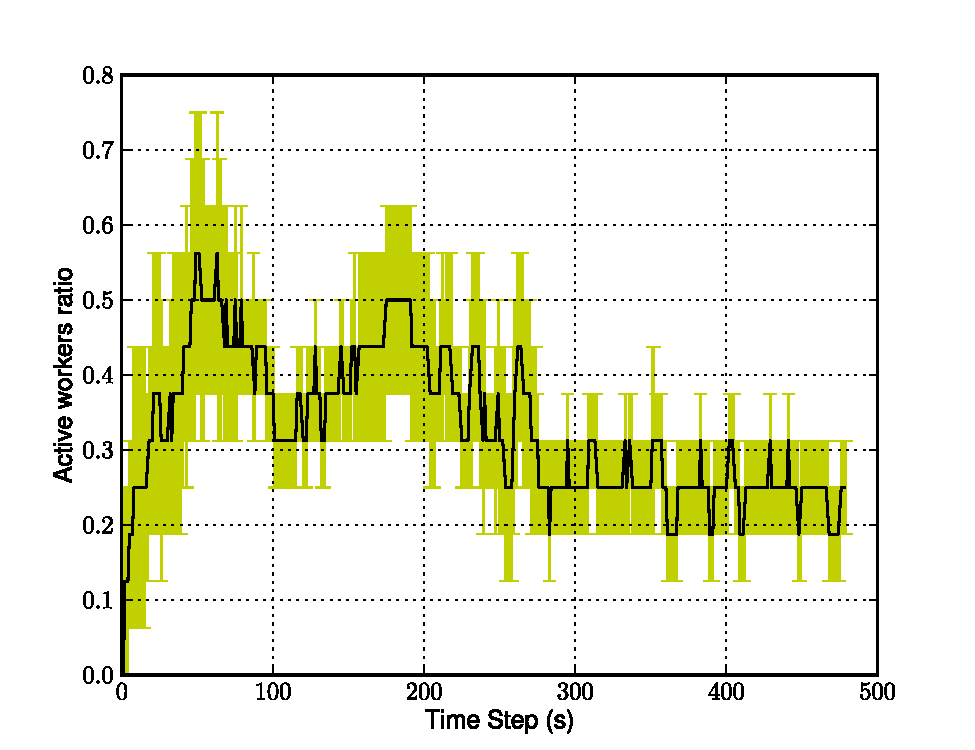
\includegraphics[width=0.7\linewidth, angle=0]
{images/SB-WorkerRatio.eps}}
\newline
\subfloat[Series C]
{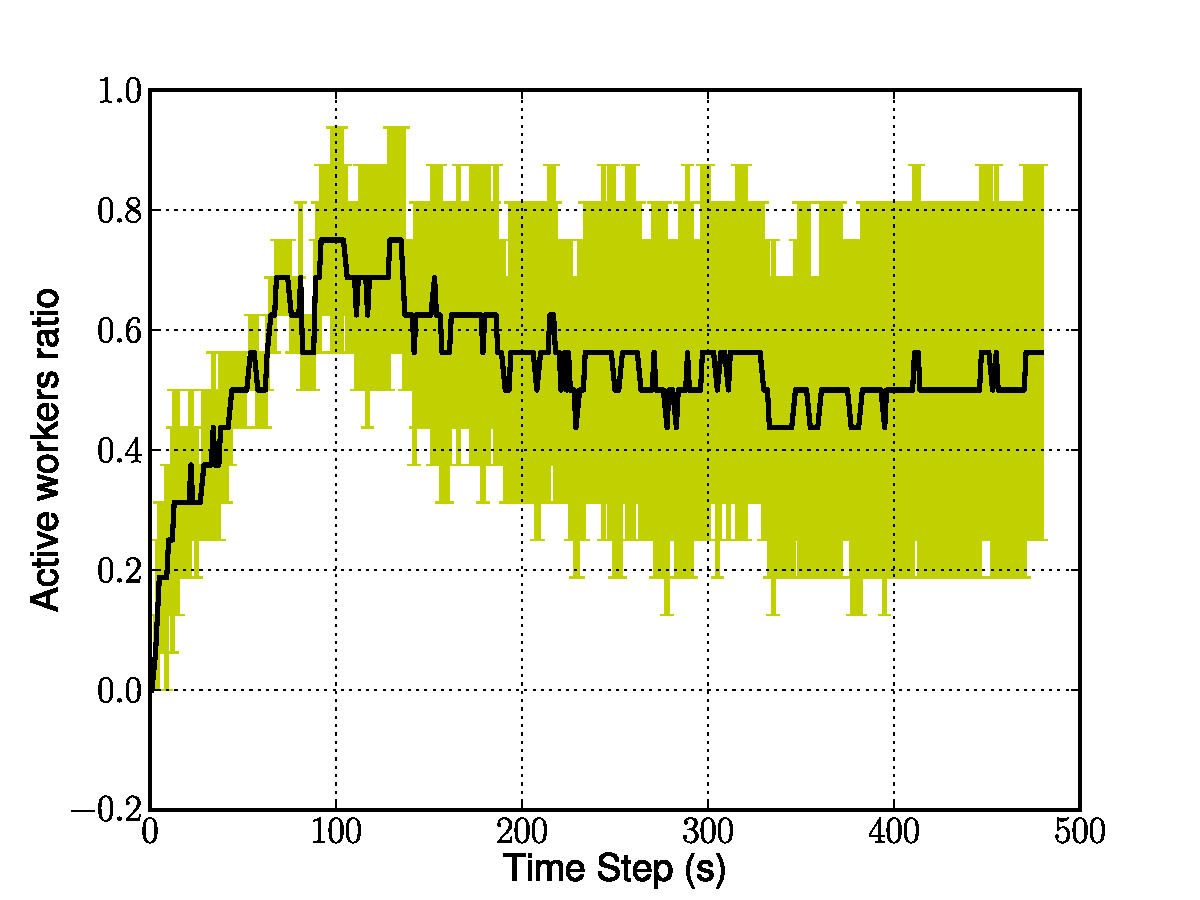
\includegraphics[width=0.7\linewidth, angle=0]
{images/SC-Local50cm-Plasticity.eps}}
%\hspace{0.2cm}
\newline
\subfloat[Series D]
{\includegraphics[width=0.7\linewidth, angle=0]
{images/SD-Local1m-Plasticity.eps}}
\newline
\caption{Self-organized allocation of robots.} 
\label{fig:worker-stat}
\end{figure}
%%
From Fig. \ref{fig:worker-stat}, we can  see that in production stage, when work-load is high, many robots are active in tasks. Here active workers ratio is the ratio of those robots that work on tasks to the total number of robots $N$ of a particular experiment.   Here we can see that this ratio varies according to the shop-floor work-load changes.
%%-------------------------------------------------------------
\subsection{Shop-task performance}
%%
\begin{figure}
\begin{centering}
\subfloat[APCD]
{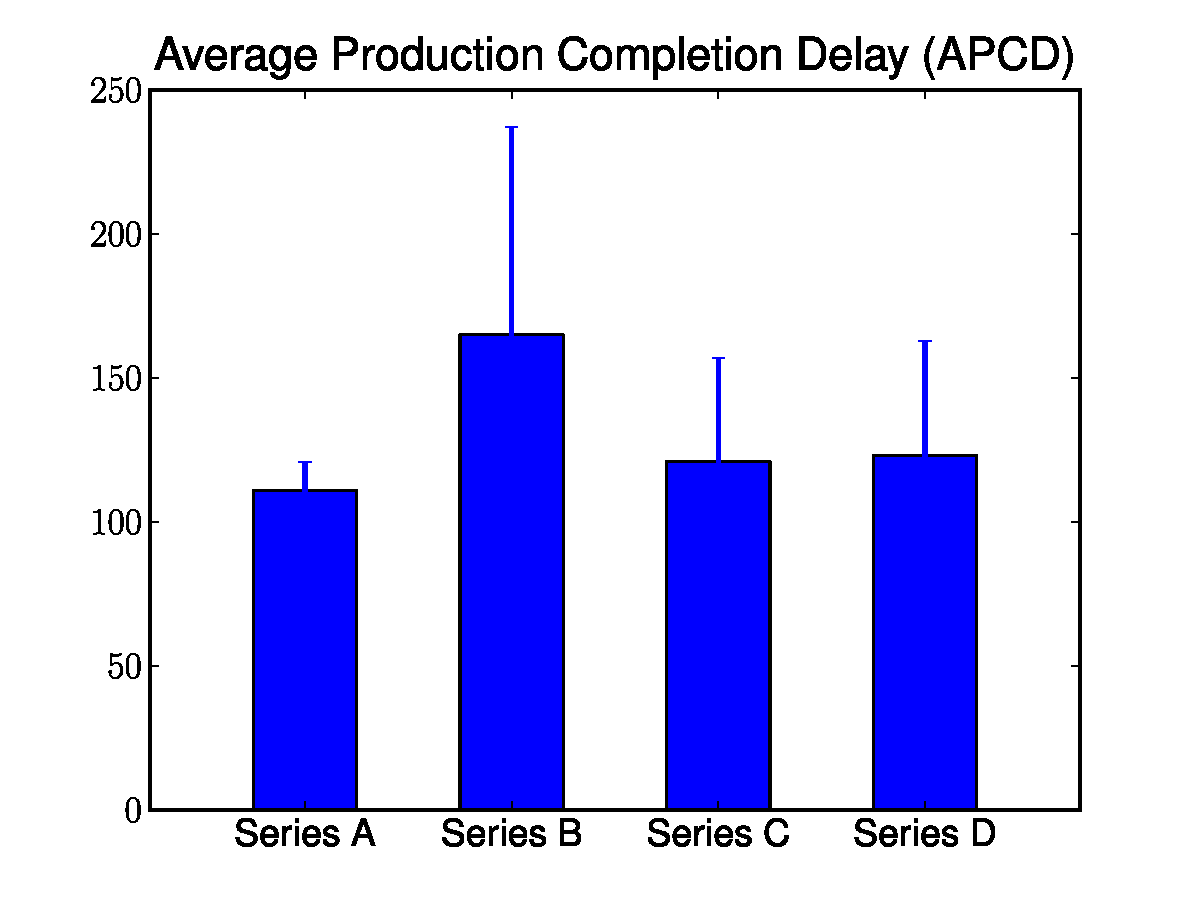
\includegraphics[width=0.7\linewidth, angle=0]
{images/apcd.eps}}
%\hspace{0.2cm}
\newline
\subfloat[APMW]
{\includegraphics[width=0.7\linewidth, angle=0]
{images/apmw.eps}}
\newline
\caption{Performance of manufacturing shop-floor tasks.} 
\end{centering}
\label{fig:mfg-stat} 
\end{figure}
%%
In our manufacturing shop-floor scenario, we have calculated the APCD and APMW as shown in Fig. \ref{fig:mfg-stat}. For Series A we have got  average production completion time 111 time-steps (555s) where sample size is (5 x 2) = 10 tasks, SD = 10 time-steps (50s). According to Eq. \ref{eqn:min-pmm}, our theoretical minimum production completion time is 50 time-steps (250s) assuming the non-stop task performance of all 8 robots with an initial task urgency of 0.5 for 2 tasks and task urgency decrease rate $\Delta \Phi_{DEC }$ = 0.0025 per robot per time-step.  Hence, Eq. \ref{eqn:appd} gives us APCD, $\zeta$ = 1.22 which means that in Series A experiments, it took 1.22 times more time (305s) than the estimated minimum production completion time (250s). For Series B, we have got average production completion time 165 time-steps (825s) where sample size is (5 x 4) = 20 tasks, SD = 72 time-steps (360s).  Hence, Eq. \ref{eqn:appd} gives us APCD, $\zeta$ = 2.3. For Series C we have got average production completion time 121 time-steps (605s) with SD = 36 time-steps (180s). For Series D,  average production completion time is 123 time-steps (615s) with SD = 40 time-steps (200s). According to Eq. \ref{eqn:min-pmm}, our theoretical minimum production completion time is 50 time-steps (250s).  The values of APCD are as follows. For Series C, $\zeta$ = 1.42 and for Series D, $\zeta$ = 1.46. For both series of experiments APCD values are very close.

For APMW, Series A experiments give us an average time length of 369 time-steps (1845s).  In this period we have calculated APMW and it is 1 time-step with SD = 1 time-step (5s) and $\Delta \Phi_{INC}$ = 0.005 per task per time-step. This shows a very low APMW ($\chi$ = 0.000235) implying a very high robustness of our system. For Series B experiments, from the average 315 time-steps (1575s) maintenance activity of our robots per experiment run, we have got APMW, $\chi$ = 0.012756 which corresponds to the pending work of 3 time-steps (15s) where SD = 13 time-steps (65s). This also tells us the robust task performance of our robots which can return to an abandoned task within a minute or so. The APMW of Series C experiments give us an average time length of 359 time-steps (1795s). In this period we calculated APMW and it is 5 time-steps with SD = 17 time-steps and $\chi$ = 0.023420. For Series D experiments, from the average 357 time-steps (1575s) of maintenance activity of our robots per experiment run, we have got APMW, $\chi$ = 0.005359 which corresponds to the pending work of 2 time-steps (10s) where SD = 7 time-steps.
%%-------------------------------------------------
\subsection{Task specializations}
We have measured the task-specialization of the robots based-on their peak value of sensitization. This maximum value represents how long a robot has repeatedly been selecting a particular task. Since tasks are homogeneous we have considered the maximum sensitization value of a robot among all tasks during an experiment run. This value is then averaged for all robots using the following  equation. 
%%
\begin{equation}
K^G_{avg} = \frac{1}{N}\sum_{i=1}^{N} \max_{j=1}^M\left ( k^i_{j, q} \right ) 
\label{eqn:K-G}
\end{equation}
%%
If a robot $r_i$ has the peak sensitization value $k^i_j$ on task $j$ ($j \in M$)  at $q^{th}$ time-step, Eq. \ref{eqn:K-G} calculates the average of the peak task-specialization values of all robots for a certain iteration of our experiments. We have also averaged the time-step values ($q$) taken to reach those peak values for all robots using the following equation.
%%
\begin{equation}
Q^G_{avg}= \frac{1}{N}\sum_{i=1}^{N} q^i_{k=k_{max}}
\label{eqn:Q-G}
\end{equation}
In Eq. \ref{eqn:Q-G}, $q^i_{k=k_{max}}$ represents the time-step of robot $r_i$  where its sensitization value $k$ reaches the peak $k_{max}$ as discussed above. By averaging this peak time-step values of all robots we can have an overall idea of how many task-execution cycles are spent to reach the maximum task-specialization value $K^G_{avg}$.
%% S-A
\begin{table}
\centering
\caption{Peak task-sensitization values of robots in a Series A experiment.}
% 30Apr expt.
\begin{tabular}{|c|c|c|c|}
\hline \textbf{Robot ID} & \textbf{Maximum k} & \textbf{At time-step (q)} & \textbf{Task} \\ 
\hline 1 & 0.54 & 64 & Task1\\
\hline 4 & 0.32 & 14 & ,,\\
\hline 5 & 0.27 & 11 & ,,\\
%%
\hline 3 & 0.47 & 63 & Task2\\
\hline 2 & 0.46 & 64 & ,,\\
\hline 6 & 0.20 & 10 & ,,\\
\hline 7 & 0.18 & 4 & ,,\\
\hline 8 & 0.15 & 3 & ,,\\
\hline 
\end{tabular} 
\label{table:K-G-SA}
\end{table}
%% S - B
\begin{table}
\centering
\caption{Peak task-sensitization values of robots in a Series B experiment.}
\begin{tabular}{|c|c|c|c|}
% Apr 18 Feb-3 expt
\hline \textbf{Robot ID} & \textbf{Maximum k} & \textbf{At time-step (q)} & \textbf{Task} \\
\hline 24 & 0.41 & 29 & Task1\\
\hline 13 & 0.31 & 19 & ,,\\
\hline 16 & 0.18 & 4 & ,,\\
%% 
\hline 1 & 0.64 & 66 & Task2\\
\hline 35 & 0.34 & 12 & ,,\\
\hline 5 & 0.28 & 14 & ,,\\
\hline 22 & 0.18 & 20 & ,,\\
\hline 17 & 0.16 & 6 & ,,\\
\hline 3 & 0.14 & 12 & ,,\\
%%
\hline 9 & 0.68 & 66 & Task3\\
\hline 6 & 0.43 & 71 & ,,\\
\hline 15 & 0.19 & 4 & ,,\\
\hline 14 & 0.15 & 4 & ,,\\
\hline 31 & 0.14 & 4 & ,,\\
%%
\hline 19 & 0.22 & 12 & Task4\\
\hline 12 & 0.16 & 10 & ,,\\
\hline 
\end{tabular} 
\label{table:K-G-SB}
\end{table}
Table \ref{table:K-G-SA} and Table \ref{table:K-G-SB} show the peak sensitization values of Series A and Series B experiments respectively.  Based on Eq. \ref{eqn:K-G} and Eq. \ref{eqn:Q-G}, we have got the peak task-sensitization $K^G_{avg} 
$ values: 0.40 (SD=0.08)  and 0.30 (SD=0.03), and their respective time-step $Q^G_{avg}$ values: 38 (SD=13) and 18 (SD=5) time-step.  They are shown in Fig. \ref{fig:task-specialization}. Here we can see that the robots in Series A had higher chances of task-specialization than that of Series B experiments.
%%
% Series C raw data
\begin{table}
\centering
\caption{Peak task-sensitization values of robots in a Series C experiment.}
% 16Feb-1 expt
\begin{tabular}{|c|c|c|c|}
\hline\textbf{ Robot ID} & \textbf{Maximum k} & \textbf{At time-step (q)} & \textbf{Task} \\
\hline 16 & 1.00 & 52 & Task1\\
\hline 12 & 0.58 & 24 & ,,\\  
\hline 1 & 0.16 & 2 & ,,\\ 
\hline 13 & 0.13 & 1 & ,,\\
%%
\hline 9 & 1.00 & 41 & Task2\\
\hline 3 & 0.55 & 23 & ,,\\ 
\hline 19 & 0.24 & 6 & ,,\\
\hline 35 & 0.24 & 6 & ,,\\
\hline 15 & 0.13 & 1 & ,,\\
\hline 33 & 0.13 & 2 & ,,\\ 
%%
\hline 6 & 0.61 & 29 & Task3\\
\hline 31 & 0.59 & 35 & ,,\\ 
\hline 5 & 0.13 & 1 & ,,\\ 
%%
\hline 17 & 0.36 & 10 & Task4\\
\hline 20 & 0.09 & 1 & ,,\\ 
\hline 22 & 0.09 & 1 & ,,\\ 
 \hline 
\end{tabular} 
\label{table:K-Q-SC}
\end{table}
%% Series D
\begin{table}
\centering
\caption{Peak task-sensitization values of robots in a Series D experiment.}
%% 17 feb-1 expt
\begin{tabular}{|c|c|c|c|}
\hline\textbf{ Robot ID} & \textbf{Maximum k} & \textbf{At time-step (q)} & \textbf{Task} \\
\hline 19 & 1.00 & 34 & Task1\\
\hline 35 & 1.00 & 60 & ,,\\
\hline 24 & 0.41 & 16 & ,,\\
\hline 12 & 0.20 & 6 & ,,\\  
%%
\hline 1 & 1.00 & 41 & Task2\\
\hline 31 & 1.00 & 47 & ,,\\
\hline 22 & 0.40 & 10 & ,,\\
\hline 9 & 0.38 & 12 & ,,\\
\hline 15 & 0.16 & 2 & ,,\\
\hline 33 & 0.13 & 1 & ,,\\ 
%%   
\hline 5 & 0.92 & 70 & Task3\\ 
\hline 13 & 0.74 & 36 & ,,\\
%% 
\hline 17 & 0.76 & 62 & Task4\\ 
\hline 6 & 0.22 & 4 & ,,\\ 
\hline 3 & 0.13 & 2 & ,,\\
\hline 16 & 0.13 & 1 & ,,\\ 
\hline 
\end{tabular}
\label{table:K-Q-SD} 
\end{table}
%%
\begin{figure}
\centering
\subfloat[Task-sensitization (K)]
{\includegraphics[width=0.7\linewidth, angle=0]
{images/K-Group.eps}}
%\hspace{0.2cm}
\newline
\subfloat[Time-steps (Q)]
{\includegraphics[width=0.7\linewidth, angle=0]
{images/Q-Group.eps}}
\newline
\caption{ Overall task-specialization of robot groups based on Peak task-sensitization values.}
\label{fig:task-specialization} 
\end{figure}
%%
%% ------ Single robot----
\begin{figure}
\centering
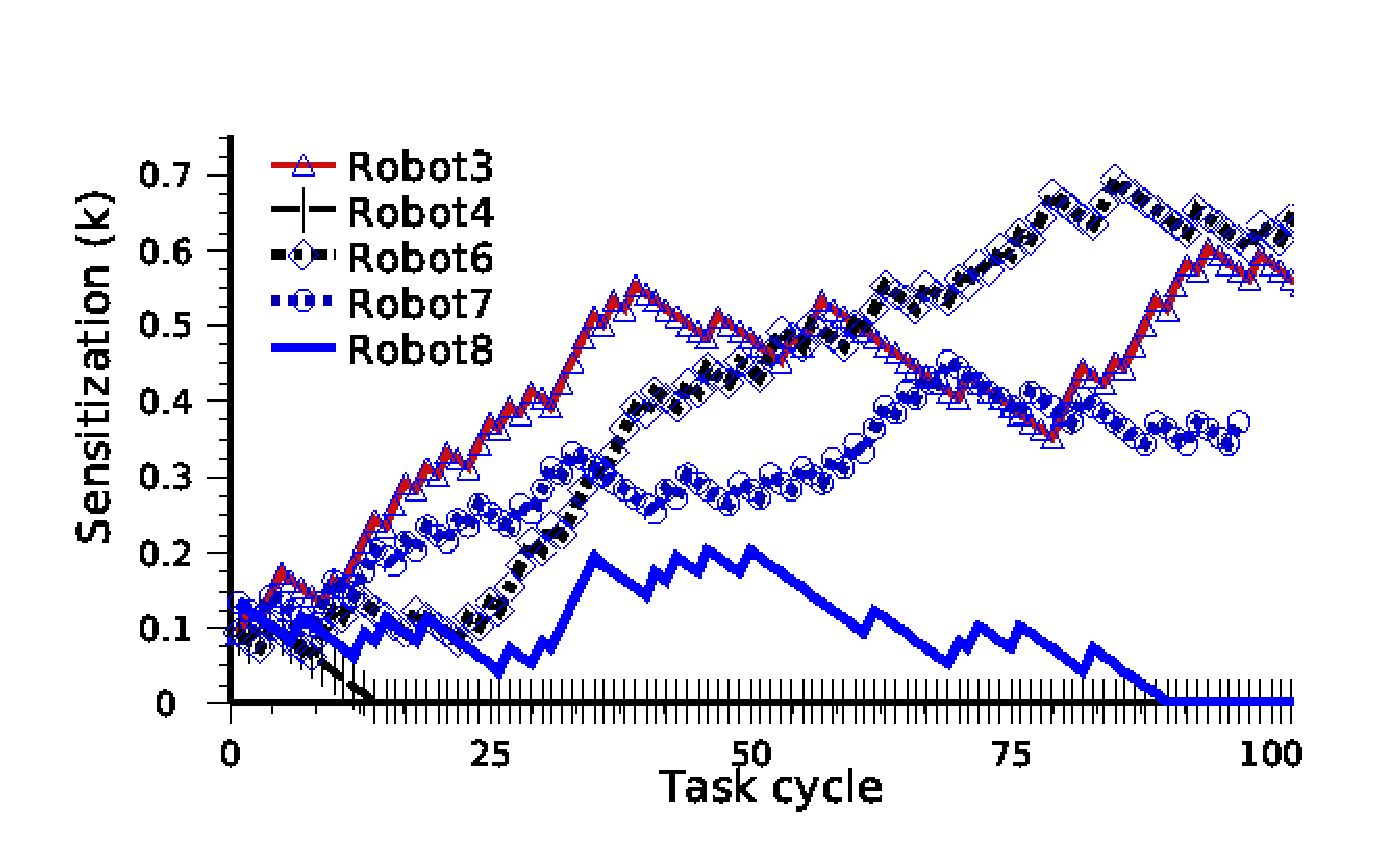
\includegraphics[width=\linewidth, angle=0]{images/TaskSpecialization-task3-10may-1.eps}
\caption{Task specialization on Task3 for a Series B experiment.}
\label{fig:k-single-task-SB} 
\end{figure}
%%
Fig. \ref{fig:k-single-task-SB} shows us the task specialization of five robots on \textit{Task3} in a particular run of Series B experiment. This shows us how some of the robots can specialize (learn) and de-specialize (forget) tasks over time.
%%-------------------------------------------------
\subsection{Robot motions}
We have aggregated the changes in translation motion of all robots over time based on their travelled distances in Euclidean metric. Let $u_{i,q}$ and $u_{i,q+1}$ be the translations of a robot $i$ in two consecutive steps. If the difference between these two translations be $\delta u_{i}$, we can find the sum of changes of translations of all robots in $(q+1)^{th}$ step using the following equation.
\begin{equation}
\Delta U_{q+1} = \sum_{i=1}^{N} \delta u_{i, q+1} 
\label{eqn:Delta-Tr}
\end{equation}
%%
\begin{figure}
\centering
\subfloat[Series A]
{\includegraphics[width=0.7\linewidth, angle=0]
{images/SA-8robots-DeltaTranslationStat.eps}}
%\hspace{0.2cm}
\newline
\subfloat[Series B]
{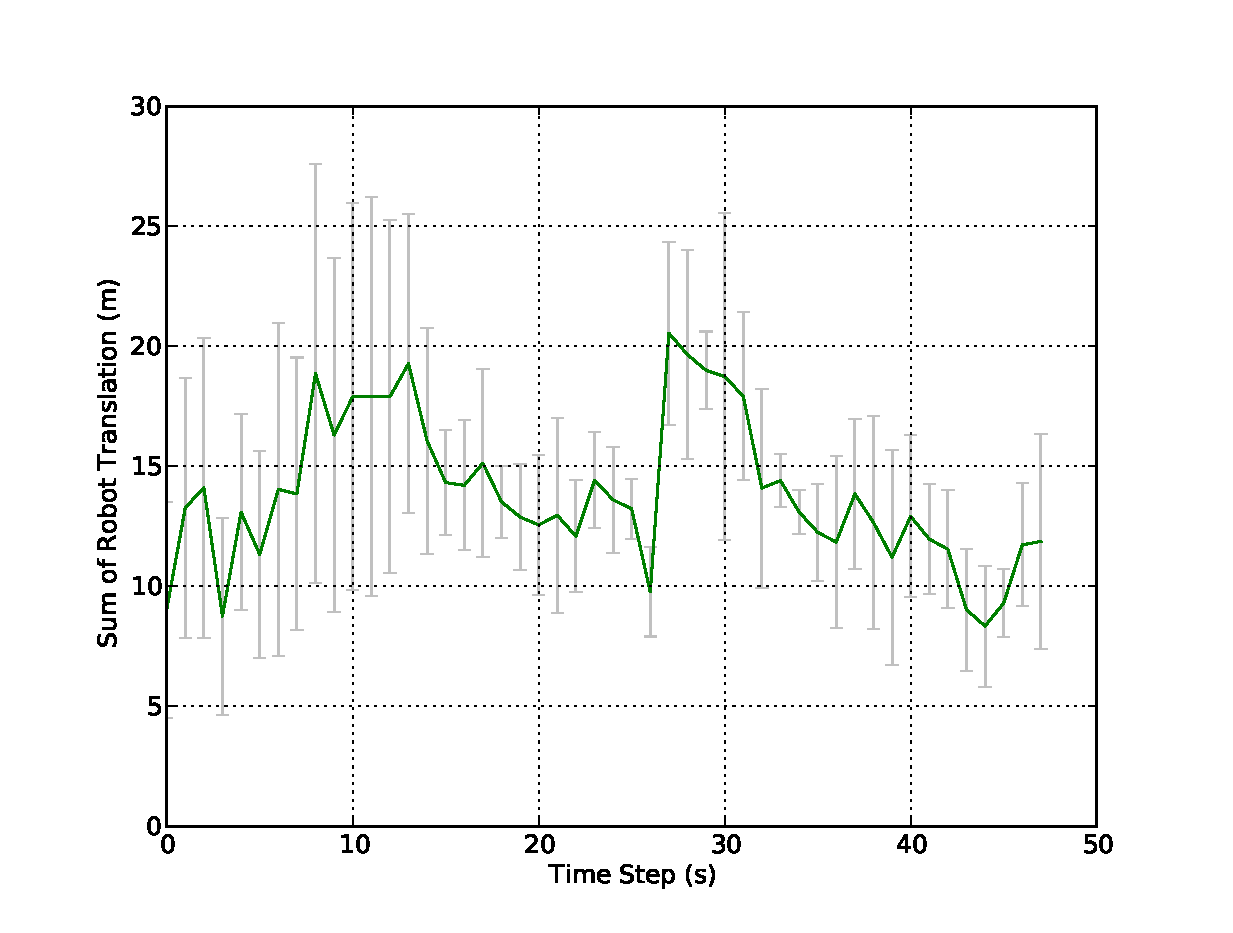
\includegraphics[width=0.7\linewidth, angle=0]
{images/SB-DeltaTranslationStat.eps}}
\newline
\subfloat[Series C]
{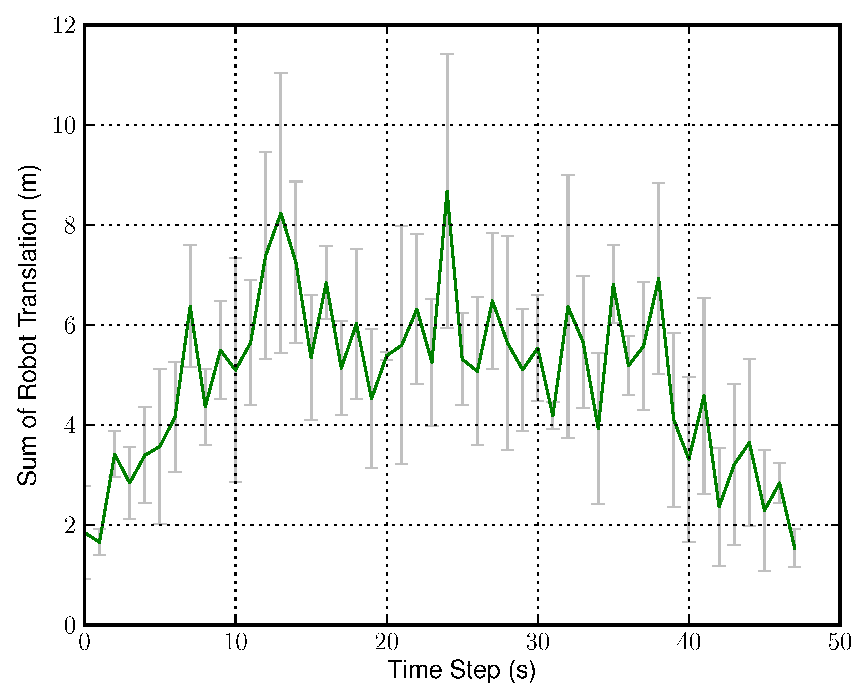
\includegraphics[width=0.6\linewidth, angle=0]
{images/SC-DeltaTranslationStat.eps}}
\newline
\subfloat[Series D]
{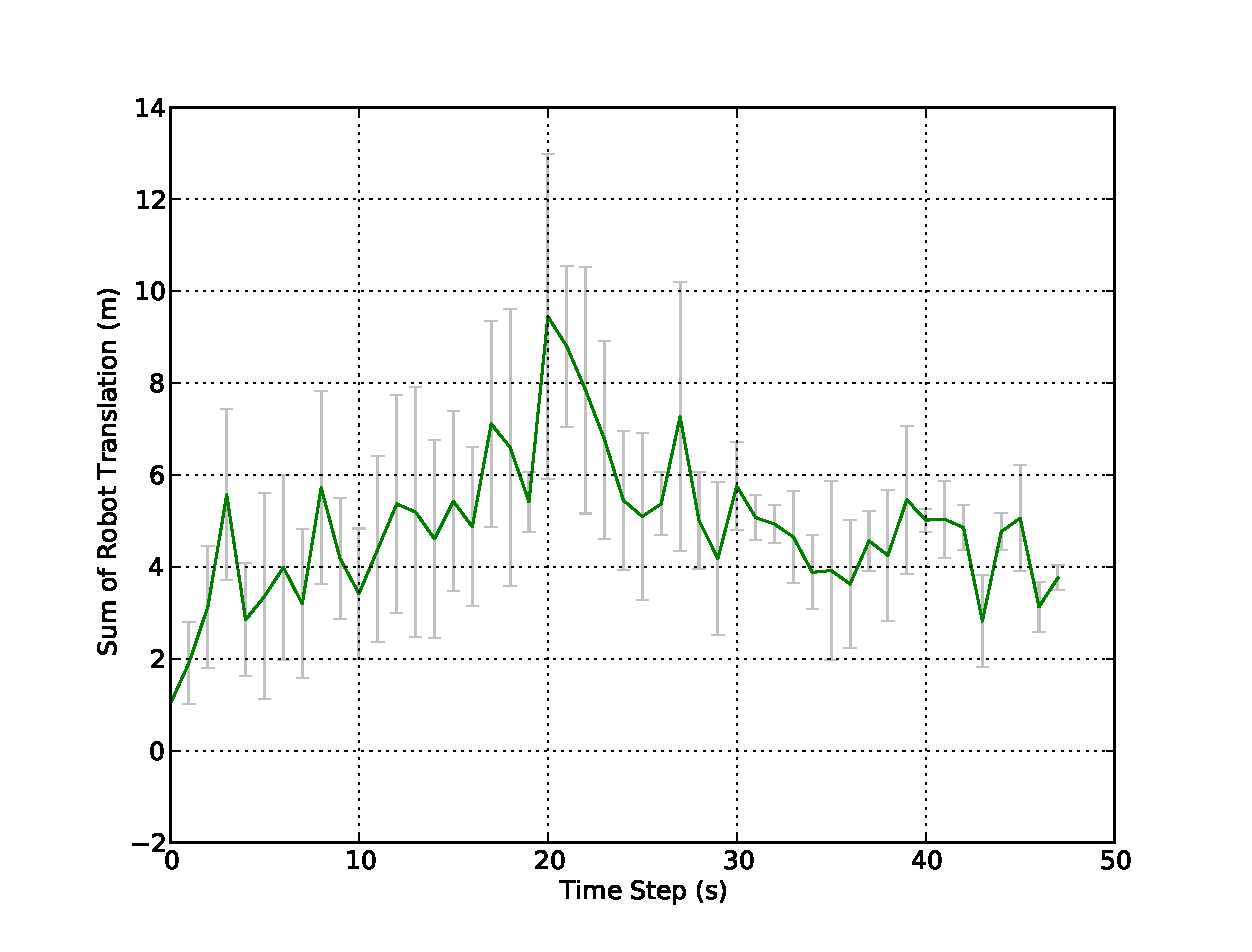
\includegraphics[width=0.7\linewidth, angle=0]
{images/SD-DeltaTranslationStat.eps}}
\newline 
\caption{Sum of the translations of robots}
\label{fig:translation-stat}
\end{figure}
%%
The sum of translations of robots from our experiments are plotted in Fig. \ref{fig:translation-stat}. In this plot we can see that robot translations also vary over varying task requirements of tasks.
%%%-------------------------------------------------
\subsection{Communication load}
%%% Communication load 
%%
\begin{figure}
\centering
\subfloat[Series A]
{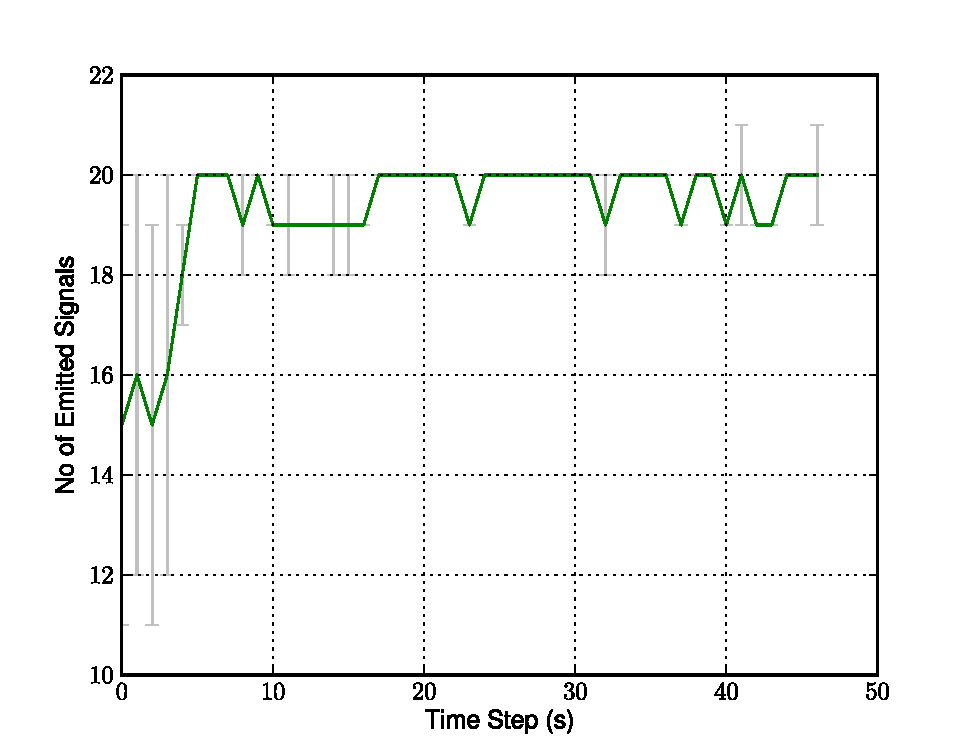
\includegraphics[width=0.7\linewidth, angle=0]
{images/SA-8Robot-SignalingFreqStat.eps}}
%\hspace{0.2cm}
\newline
\subfloat[Series B]
{\includegraphics[width=0.7\linewidth, angle=0]
{images/SB-SignalingFreqStat.eps}}
\newline
\subfloat[Series C]
{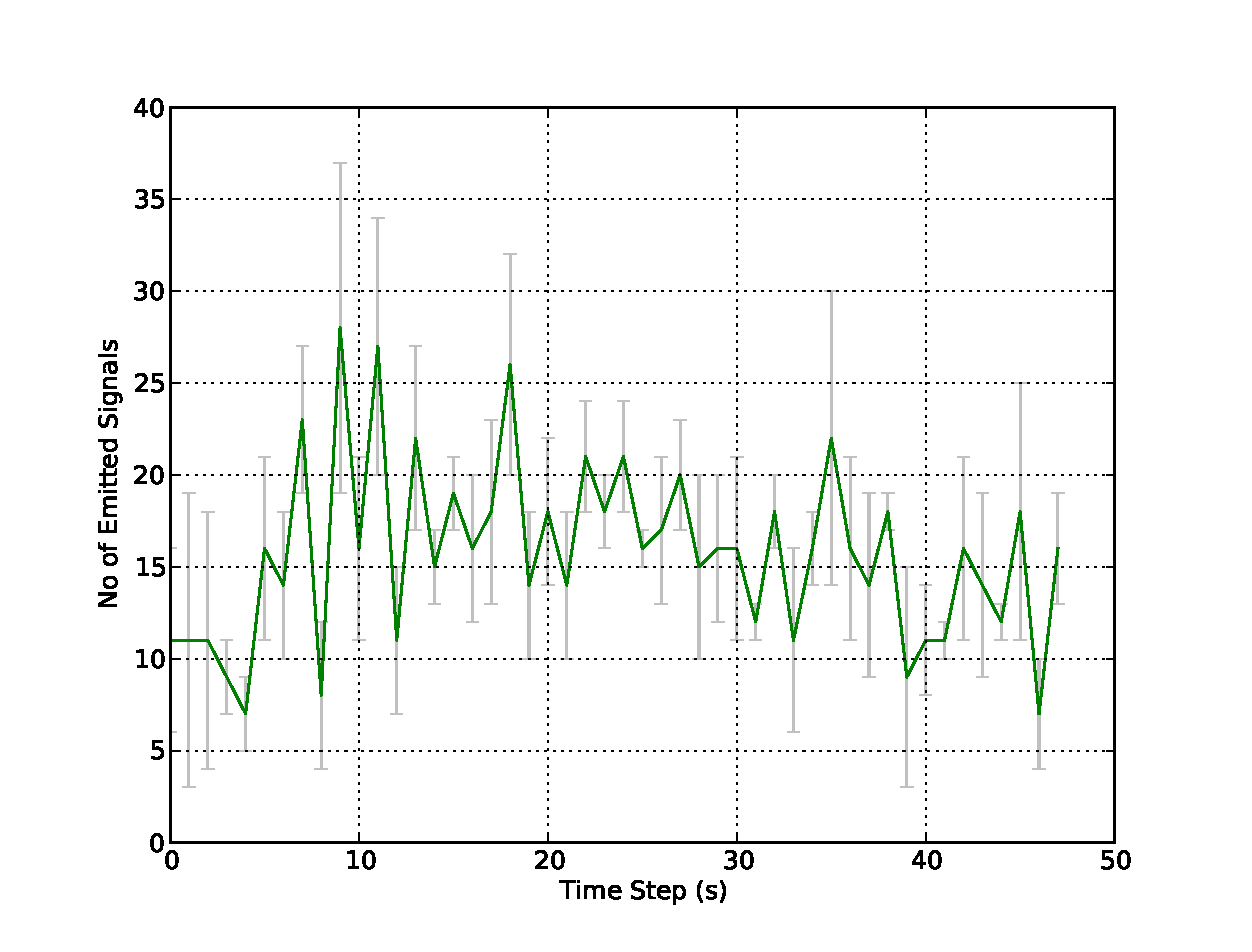
\includegraphics[width=0.7\linewidth, angle=0]
{images/SC-Local-500cm-SignalingFreqStat.eps}}
%\hspace{0.2cm}
\newline
\subfloat[Series D]
{\includegraphics[width=0.7\linewidth, angle=0]
{images/SD-Local-1m-SignalingFreqStat.eps}}
\newline
\caption{Frequency of \texttt{TaskInfo} signalling of (a) and (b) by TPS and (c) and (d) by local peers.}
\label{fig:signal-frequency-stat}
\end{figure}
%%
%%%% Single robot- number of peers
\begin{figure}
\begin{centering}
\subfloat[Series C]{\includegraphics[width=0.7\linewidth]{images/Robot12-16feb-1-LocalSignals.eps}}
\newline
\subfloat[Series D]{\includegraphics[width=0.7\linewidth]{images/Robot12-17feb-3-LocalSignals.eps}}
\newline
\caption{\small \texttt{LoaclTaskInfo} (P2P) signals caught by Robot12 in (a) Series C and (b) Series D experiment}
\end{centering}
\label{fig:local-single-robot-signal}
\end{figure}
%%
Fig. \ref{fig:signal-frequency-stat} (a) and (b) shows the number of received \texttt{TaskInfo} signals by each robot in Series A and Series B experiments. Since the duration of each time-step is 50s long and TPS emits signal in every 2.5s, there is an average of 20 signals in each time-step. The overall P2P task information signals of both of these local modes are plotted in Fig. \ref{fig:signal-frequency-stat} (c) and (d). As an example of P2P signal reception of a robot,  Fig. \ref{fig:local-single-robot-signal} show the number of received signals by \textit{Robot12} in two local experiments. It states the relative difference of peers over time in two different cases.
%==================================================================
\section{Discussions}
\label{sec:discuss}
%%
\subsection{Self-regulated MRTA}
From our experimental results, we have noted several aspects of self-regulated MRTA that expose the effectiveness of AFM. As we have pointed out that this self-regulated MRTA, as observed in biological and human social systems, needs to satisfy several important characteristics, particularly plasticity and task-specialization. In addition to satisfying those basic qualities, AFM has demonstrated many other aspects. Our self-regulated robots, driven by AFM, effectively handle the dynamic work-load in our manufacturing shop-floor. They can dynamically support the need to work on demanding tasks, if there any. The variations of active worker ratio shows this. 

From the self-organized worker allocations of AFM, it is clear to us that although in larger system (Series B) the degree of variations of active-worker ratio can show us significantly unpredictable patterns, nevertheless the self-regulated rules drive the robots to respond to the dynamic needs of the system. This means that AFM can sufficiently produce the plasticity of DOL in order to meet the dynamic work-load of the system.
%%
\subsection{Learning and forgetting} 
From the individual and group-level task-specialization, we can see that robots can maintain both task-specialization and flexibility. In a self-organized system, it is very common that only a few individuals specialize on tasks and others generally do not. From two sample data sets provided in Table \ref{table:K-G-SA} and Table \ref{table:K-G-SB}, we can see that in particular runs of Series A and Series B experiments, task-sensitization values of  only 2-3 robots reach above the group-level average score. Thus in both types of experiments, robots exhibit similar task-specialization behaviours. 
%%
\subsection{Concurrency and robustness}
As a consequence of fewer robots specializing in tasks, we can also see that robots can concurrently  consider different tasks without being biased to a particular task all the time. Our experiments also show us the robust MRTA as in case of  both high and low work-loads present in the system. This is evident from the manufacturing shop-floor task performance during PMM and MOM. For example,  in case of Series B experiments APMW was 13 time-steps (65s) which corresponded  to pending work-load of 0.065 unit for a single robot. Thus, on an average, before the work-load exceeded by about 13 percent of initial work-load, robots were able to respond to  a task.
%%
\subsection{Communication load}
In GSNC strategy based experiments we used a centralized communication system (source of attractive fields) that serves the robots with necessary task-perception information.  Our centralized communication system has the advantage of minimising the communication load and the disadvantage of a single point of failure as well as a single point of load. Under LSLC strategy based implementation, we present how the task perception can be decentralized by P2P communications among RCCs.
%%
\subsection{Scaling-up}
We have observed the effect of scaling-up the robot team size. The system size of Series B is double of that of Series A in terms of robots, tasks and experiment arena. Keeping a fixed ratio of robot-to-task and task-to-arena we have intended to see the scaling effects in our experiments. Here we see that both systems can show sufficient self-regulated DOL, but task-performance of both systems varies significantly. For example, the value of APCD in Series B is higher by 1.08. This means that performance  is decreased in Series B experiments despite having the resources in same proportion in both systems. This occurs partly due to the greater stochastic effects found in task-allocation in a larger system, e.g. presence of more tasks produce higher stochastic behaviours in robot's task selection.

Similarly we can see that in larger system robots have less chances to specialize on tasks, as the Series B experiments show us that the overall average task-specialization of the group $K^G_{avg}$ is lower by 0.10 and it lasts for significantly less time (the difference of $Q^G_{avg}$  of both systems is 20 time-steps). Thus, in a large group, robots are more likely to switch among tasks more frequently and this produces more translation motions which cost more energy (e.g. battery power) in task-performance.
%%
\subsection{Comparisons between GSNC and LSLC strategies} 
\begin{table}[H]
%\begin{scriptsize}
\begin{center}
\caption{Shop-floor production and maintenance task performance}
\begin{tabular}{|p{0.26in}|p{0.7in}|p{0.7in}|p{0.7in}|p{0.7in}|}
\hline Series & \textit{Production \protect\newline delay \protect\newline (SD) s} & \textit{p-value} \protect\newline 1-tailed \protect\newline t-test\protect\newline (confidence) & \textit{Pending \protect\newline maintenance time (SD) s} & \textit{p-value} 1-tailed \protect\newline t-test\\ 
\hline A & 555 (50) & 0.0 & 5 (5) & 0.0\\ 
\hline B & 825 (360) & 0.2 (60\%) & 15 (65) & 0.0 \\
\hline C & 605 (180) & N/A & 25 (85) & N/A\\
\hline D  & 615 (200) & 0.0 & 10 (35) & 0.0\\
\hline
\end{tabular}
\label{table:vsp-cmp} 
\end{center}
%\end{scriptsize}
\end{table}
Results from Series C and Series D experiments show many similarities and differences with respect to the results of Series A and Series B experiments. As shown in Table \ref{table:vsp-cmp}  both Series C and Series D experiments show similar production delay (APCD) values: 605s and 615s respectively, which are less than Series B experiment result (825s) and are close to Series A experiment result (555s). Note that all statistical t-test results are obtained with respect to Series C data and it shows that there is no significant difference in task-performance between Series B and Series C results.
%%
\begin{table}[H]
%\begin{scriptsize}
\begin{center}
\caption{Task-specialization values of the robots}
\begin{tabular}{|p{0.26in}|p{0.7in}|p{0.7in}|c|p{0.7in}|}
\hline Series & $ K^G_{avg}$ (SD) & \textit{ p-value} \protect\newline 1-tailed t-test \protect\newline (confidence)  & $ Q^G_{avg}$ (SD) & \textit{ p-value} \protect\newline 1-tailed \protect\newline t-test \protect\newline (confidence) \\ 
\hline A & 0.40 (0.08)& 0.0 & 38 (13) & 0.001 (99.8\%)\\ 
\hline B &  0.30 (0.03) & 0.2 (60\%) &  18 (5) & 0.2 (60\%)\\
\hline C  & 0.39 (0.17) & N/A & 13 (7) & N/A \\
\hline D  & 0.27 (0.1)& 0.0 & 11 (5) & 0.0\\
\hline
\end{tabular}
\label{table:k-cmp} 
\end{center}
%\end{scriptsize}
\end{table}
Besides, in terms of task-specialization as shown in Table \ref{table:k-cmp}, the overall task-specialization of group in Series C ($K^G_{avg}$ = 0.4) is  closer to that of Series A experiments ($K^G_{avg}$ = 0.39) and interestingly, the value of  Series D ($K^G_{avg}$ = 0.27) is  much closer to that of Series B experiments ($K^G_{avg}$ = 0.30). So task-specialization in large group under LSLC strategy is not significantly different than their GSNC counter part. %Besides task-specialization happens much faster under LSLC strategy as it can be seen that the average time to reach peak sensitization values  of the group,  $Q^G_{avg}$ in Series C is lower than that of Series A values by 25 time-steps.

\begin{table}[H]
%\begin{small}
\begin{center}
\caption{Sum of translations of robots in all experiments.}
\begin{tabular}{|p{0.3in}|p{1in}|p{0.9in}|}
\hline Series & Average \protect\newline translation \protect\newline(SD) m & \textit{p-value} \protect\newline 1-tailed t-test (confidence)\\ 
\hline A & 2.631 (0.804) & N/A\\ 
\hline B & 13.882 (3.099) & 0.001 (99.8\%)\\
\hline C & 4.907 (1.678) & N/A\\
\hline D  & 4.854  (1.592) & 0.0\\
\hline
\end{tabular}
\label{table:motion-cmp} 
\end{center}
%\end{small}
\end{table}
%%
Table \ref{table:motion-cmp} summarizes the average translations done by robots in all four series of experiments. From these robot motion profiles, it is found that under LSLC strategy, robot translations have been reduced significantly. From this table it is seen than Series C and Series D show about 2.8 times less translation than that in Series B experiments. The translation of 16 robots in Series C and Series D experiments are approximately double (1.89 times) than that of Series A experiments with 8 robots.  Thus the energy-efficiency under LSLC strategy seems to be higher  than that under GSNC strategy.

From the above results one can see that large group robots achieve similar or better MRTA under LSLC strategy. The local sensing of tasks prevents them to attend a far-reaching task which may be more common under global sensing strategy. However, as it is seen in Fig. \ref{fig:raw-urgencies-SC-SD}
some tasks can be left unattended for a long period of time due to the failure to discover it by any robot. For that reason it is seen that the values of pending maintenance load is slightly higher under LSLC strategy. But this trade-off is worth as LSLC strategy provides superior self-regulated MRTA in terms of task-performance, task-specialization and energy-efficiency.
%%================================================================
\section{Conclusions}
\label{sec:conc}
The benefits of deploying a large number of robots in dynamic multi-tasking environment can not be fully realized without adopting an effective communication and sensing strategy for a given multi-robot system. This study has focused on comparing two bio-inspired  communication and sensing strategies in producing self-regulated MRTA by an interdisciplinary model of DOL, AFM. Under the GSNC strategy, AFM has produced the desired self-regulated MRTA among a group of 8 and 16 robots. This gives us the evidence that AFM can successfully solve the MRTA issue of a complex multi-tasking environment like a manufacturing shop-floor. Under the LSLC strategy, AFM can also produce the desired self-regulated MRTA for 16 robots with different communication and sensing ranges.

From our comparative results, we note that for large group of robots,  degradation in  task-performance and task-specialization of robots are likely to occur  under GSNC strategy that relies upon a centralized communication system. Thus GSNC strategy can give us better performance when the number of tasks and robots are relatively small. This confirms us the assertions made by some biologists that self-regulated DOL among small group of individuals can happen without any significant amount of local communications and interactions. However, our findings suggest that task-specialization can still be beneficial among the individuals of a small group which contradicts the claim that small groups only posses the generalist workers, but not the specialists.

On the other hand, LSLC strategy is more suitable for large group of individuals that are likely to be unable to perform global sensing and global communications with all individuals of the group. The design of communication and sensing range has still remained as a critical research issue. However, our results suggest that the idea of maximizing information gain is not appropriate under a stochastic task-allocation process. Here more information tends to cause more task-switching behaviours that lowers the level of task-specialization of the group. This might not be the case under a deterministic task-allocation scheme where more information may lead to better and optimum allocations in  a small group of individuals. Nevertheless, despite having the limited communication and sensing range, LSLC strategy has helped the robots to produce comparatively better task-allocation with increased task-specialization and significantly reduced motions or savings in energy consumption.
%%========================================================================
\section*{Acknowledgement}
This research has been funded by the Engineering and Physical Sciences Research Council (EPSRC), UK, grant reference EP/E061915/1.
%%===========================================================
%% The Appendices part is started with the command \appendix;
%% appendix sections are then done as normal sections
%% \appendix%% \section%% \label{}
%% References
%%
%% Following citation commands can be used in the body text:
%% Usage of \cite is as follows:
%%   \cite{key}         ==>>  [#]
%%   \cite[chap. 2]{key} ==>> [#, chap. 2]
%%

%% References with bibTeX database:
\bibliographystyle{./elsart/elsarticle-num}
\bibliography{ras1}
%% Authors are advised to submit their bibtex database files. They are
%% requested to list a bibtex style file in the manuscript if they do
%% not want to use elsarticle-num.bst.
%% References without bibTeX database:
% \begin{thebibliography}{00}
%% \bibitem must have the following form:
%%   \bibitem{key}...
%%
% \bibitem{}
% \end{thebibliography}
\end{document}
%%
%% End of file `elsarticle-template-num.tex'.